%%% The main file. It contains definitions of basic parameters and includes all other parts.

%% Settings for single-side (simplex) printing
% Margins: left 40mm, right 25mm, top and bottom 25mm
% (but beware, LaTeX adds 1in implicitly)
\documentclass[12pt,a4paper]{report}
\setlength\textwidth{145mm}
\setlength\textheight{247mm}
\setlength\oddsidemargin{15mm}
\setlength\evensidemargin{15mm}
\setlength\topmargin{0mm}
\setlength\headsep{0mm}
\setlength\headheight{0mm}
% \openright makes the following text appear on a right-hand page
\let\openright=\clearpage

%% Settings for two-sided (duplex) printing
% \documentclass[12pt,a4paper,twoside,openright]{report}
% \setlength\textwidth{145mm}
% \setlength\textheight{247mm}
% \setlength\oddsidemargin{14.2mm}
% \setlength\evensidemargin{0mm}
% \setlength\topmargin{0mm}
% \setlength\headsep{0mm}
% \setlength\headheight{0mm}
% \let\openright=\cleardoublepage

%% Generate PDF/A-2u
\usepackage[a-2u]{pdfx}

%% Character encoding: usually latin2, cp1250 or utf8:
\usepackage[utf8]{inputenc}

%% Prefer Latin Modern fonts
\usepackage{lmodern}

%% Further useful packages (included in most LaTeX distributions)
\usepackage{amsmath}        % extensions for typesetting of math
\usepackage{amsfonts}       % math fonts
\usepackage{amsthm}         % theorems, definitions, etc.
\usepackage{bbding}         % various symbols (squares, asterisks, scissors, ...)
\usepackage{bm}             % boldface symbols (\bm)
\usepackage{graphicx}       % embedding of pictures
\usepackage{fancyvrb}       % improved verbatim environment
\usepackage{natbib}         % citation style AUTHOR (YEAR), or AUTHOR [NUMBER]
\usepackage[nottoc]{tocbibind} % makes sure that bibliography and the lists
			    % of figures/tables are included in the table
			    % of contents
\usepackage{dcolumn}        % improved alignment of table columns
\usepackage{booktabs}       % improved horizontal lines in tables
\usepackage{paralist}       % improved enumerate and itemize
\usepackage{xcolor}         % typesetting in color

% noarr
\usepackage{subcaption}
\usepackage{minted}
\usemintedstyle{vs}
\definecolor{LightGray}{gray}{0.96}
\newmintedfile[inputmintedcpp]{c++}{bgcolor=LightGray,tabsize=2,fontsize=\scriptsize,linenos, breaklines,escapeinside=\#\#}
\usepackage{listings}
\definecolor{codegray}{rgb}{0.5,0.5,0.5}
\definecolor{backcolour}{rgb}{0.95,0.95,0.92}
\lstset{basicstyle=\scriptsize\ttfamily,%
    language=c++,%
    keywordstyle=\color{blue},%
    stringstyle=\color{magenta},%
    commentstyle=\color{green!50!black},%
    showstringspaces=false,%
    rulecolor=\color{lightgray},%
    backgroundcolor=\color{backcolour},   
    numberstyle=\tiny\color{codegray},
    breakatwhitespace=false,         
    breaklines=true,                 
    captionpos=b,                    
    keepspaces=true,                 
    numbers=left,                    
    tabsize=2,
    otherkeywords={size_t},
}


%%% Basic information on the thesis

% Thesis title in English (exactly as in the formal assignment)
\def\ThesisTitle{Employing Parallel Computing in Data-Intensive Tasks}

% Author of the thesis
\def\ThesisAuthor{Adam Šmelko}

% Year when the thesis is submitted
\def\YearSubmitted{2024}

% Name of the department or institute, where the work was officially assigned
% (according to the Organizational Structure of MFF UK in English,
% or a full name of a department outside MFF)
\def\Department{Department of Distributed and Dependable Systems}

% Is it a department (katedra), or an institute (ústav)?
\def\DeptType{Department}

% Thesis supervisor: name, surname and titles
\def\Supervisor{Martin Kruliš}

% Supervisor's department (again according to Organizational structure of MFF)
\def\SupervisorsDepartment{Department of Distributed and Dependable Systems}

% Study programme and specialization
\def\StudyProgramme{Computer Science}
\def\StudyBranch{Software Systems}

% An optional dedication: you can thank whomever you wish (your supervisor,
% consultant, a person who lent the software, etc.)
\def\Dedication{%
Dedication.
}

% Abstract (recommended length around 80-200 words; this is not a copy of your thesis assignment!)
\def\Abstract{%
Abstract.
}

% 3 to 5 keywords (recommended), each enclosed in curly braces
\def\Keywords{%
{key} {words}
}

%% The hyperref package for clickable links in PDF and also for storing
%% metadata to PDF (including the table of contents).
%% Most settings are pre-set by the pdfx package.
\hypersetup{unicode}
\hypersetup{breaklinks=true}

% Definitions of macros (see description inside)
%%% This file contains definitions of various useful macros and environments %%%
%%% Please add more macros here instead of cluttering other files with them. %%%

%%% Minor tweaks of style

% This macro defines a chapter, which is not numbered, but is included
% in the table of contents.
\def\chapwithtoc#1{
\chapter*{#1}
\addcontentsline{toc}{chapter}{#1}
}

\def\secwithtoc#1{
\section*{#1}
\addcontentsline{toc}{section}{#1}
}

% Draw black "slugs" whenever a line overflows, so that we can spot it easily.
\overfullrule=5mm
\emergencystretch=1cm

\AtBeginDocument{
\hyphenation{SOM-Hun-ter}
\hyphenation{Wi-de-spread}
}

%%% Macros for definitions, theorems, claims, examples, ... (requires amsthm package)

\theoremstyle{plain}
\newtheorem{thm}{Theorem}
\newtheorem{lemma}[thm]{Lemma}
\newtheorem{claim}[thm]{Claim}

\theoremstyle{plain}
\newtheorem{defn}{Definition}
\newtheorem{problem}{Problem}

\theoremstyle{remark}
\newtheorem*{cor}{Corollary}
\newtheorem*{rem}{Remark}

%%% An environment for proofs

\newenvironment{myproof}{
  \par\medskip\noindent
  \textit{Proof}.
}{
\newline
\rightline{$\qedsymbol$}
}

%%% The field of all real and natural numbers
\newcommand{\R}{\mathbb{R}}
\newcommand{\N}{\mathbb{N}}
\newcommand{\Asymp}[1]{\ensuremath{\mathcal{O}\left(#1\right)}}

%%% Useful operators for statistics and probability
\DeclareMathOperator{\pr}{\textsf{P}}
\DeclareMathOperator{\E}{\textsf{E}\,}
\DeclareMathOperator{\var}{\textrm{var}}
\DeclareMathOperator{\sd}{\textrm{sd}}
\DeclareMathOperator{\subs}{\textsc{Sub}}

% contributions
\newcounter{contribution}
\def\contribution#1{
\refstepcounter{contribution}
\chapter*{Contribution \arabic{contribution}\\#1}
\addcontentsline{toc}{chapter}{Contribution \arabic{contribution}\\#1}
}

\crefname{contribution}{contribution}{contributions}
\Crefname{contribution}{Contribution}{Contributions}

\setlength{\marginparpush}{0pt}
\setlength{\marginparsep}{2em}

\newcommand{\contribmark}[1]{%
\hyperref[#1]{\begin{tikzpicture}[ultra thick, font=\sf\bfseries]
\node[regular polygon, regular polygon sides=3, rounded corners=0.3ex, inner sep=.3ex,draw] (ll) {\ref*{#1}};
\end{tikzpicture}}}
\newcommand{\margincontrib}[1]{\marginnote{\contribmark{#1}}}

\newcommand{\publishedas}[1]{\begin{description}\item[Published as]\begin{refsection}\fullcite{#1}\end{refsection}\end{description}}

% ONLINE VERSION without the manuscripts
\newif\ifonlineversion
\onlineversiontrue
%\onlineversionfalse
\newcommand\onlineomit[1]{\ifonlineversion\vfill\begin{center}\fbox{\parbox{16.5em}{\footnotesize A re-printed manuscript that would appear here is omitted in the electronic version of the thesis.}}\end{center}\vfill\else#1\fi}

% publication contributions
\def\contF{\begin{tikzpicture}\fill circle(0.666ex);\end{tikzpicture}}
\def\contP{\begin{tikzpicture}\begin{scope}[rotate=90]\clip circle(0.666ex);\fill (-0.666ex,-0.666ex) rectangle(-0.1ex,0.666ex);\end{scope}\draw circle(0.666ex);\end{tikzpicture}}
\def\contN{\begin{tikzpicture}\draw[densely dotted] circle(0.666ex);\end{tikzpicture}}

% chemfig style
\renewcommand*\printatom[1]{\ensuremath{\mathsf{#1}}}
\setchemfig{atom sep=4ex, angle increment=30}
\catcode`\_=11
\tikzset{
	ddbond/.style args={#1}{
		draw=none,
		decoration={%
			markings,
			mark=at position 0 with {
				\coordinate (CF@startdeloc) at (0,\dimexpr#1\CF_doublesep/2)
				coordinate (CF@startaxis) at (0,\dimexpr-#1\CF_doublesep/2);
			},
			mark=at position 1 with {
				\coordinate (CF@enddeloc) at (0,\dimexpr#1\CF_doublesep/2)
				coordinate (CF@endaxis) at (0,\dimexpr-#1\CF_doublesep/2);
				\draw[dash pattern=on 2pt off 1.5pt] (CF@startdeloc)--(CF@enddeloc);
				\draw (CF@startaxis)--(CF@endaxis);
			}
		},
		postaction={decorate}
	}
}
\catcode`\_=8

% latexdiff preamble commands:
%DIF UNDERLINE PREAMBLE %DIF PREAMBLE
\RequirePackage[normalem]{ulem} %DIF PREAMBLE
\RequirePackage{color}\definecolor{RED}{rgb}{1,0,0}\definecolor{BLUE}{rgb}{0,0,1} %DIF PREAMBLE
\providecommand{\DIFadd}[1]{{\protect\color{green!50!black}\uwave{#1}}} %DIF PREAMBLE
\providecommand{\DIFdel}[1]{{\protect\color{red}\sout{#1}}}                      %DIF PREAMBLE
%DIF SAFE PREAMBLE %DIF PREAMBLE
\providecommand{\DIFaddbegin}{} %DIF PREAMBLE
\providecommand{\DIFaddend}{} %DIF PREAMBLE
\providecommand{\DIFdelbegin}{} %DIF PREAMBLE
\providecommand{\DIFdelend}{} %DIF PREAMBLE
\providecommand{\DIFmodbegin}{} %DIF PREAMBLE
\providecommand{\DIFmodend}{} %DIF PREAMBLE
%DIF FLOATSAFE PREAMBLE %DIF PREAMBLE
\providecommand{\DIFaddFL}[1]{\DIFadd{#1}} %DIF PREAMBLE
\providecommand{\DIFdelFL}[1]{\DIFdel{#1}} %DIF PREAMBLE
\providecommand{\DIFaddbeginFL}{} %DIF PREAMBLE
\providecommand{\DIFaddendFL}{} %DIF PREAMBLE
\providecommand{\DIFdelbeginFL}{} %DIF PREAMBLE
\providecommand{\DIFdelendFL}{} %DIF PREAMBLE


% Mahalanobis
\DeclareMathOperator{\cov}{\textbf{cov}}
\DeclareMathOperator{\mean}{mean}
\DeclareMathOperator{\argmin}{argmin}

% Title page and various mandatory informational pages
\begin{document}
%%% Title page of the thesis and other mandatory pages

%%% Title page of the thesis

\pagestyle{empty}
\hypersetup{pageanchor=false}
\begin{center}

\centerline{\mbox{
\includegraphics[width=166mm]{img/logo-en.pdf}}}

\vspace{-8mm}
\vfill

{\bf\Large DOCTORAL THESIS}

\vfill

{\LARGE\ThesisAuthor}

\vspace{15mm}

{\LARGE\bfseries\ThesisTitle}

\vfill

\Department

\vfill

{
\centerline{\vbox{\halign{\hbox to 0.45\hsize{\hfil #}&\hskip 0.5em\parbox[t]{0.45\hsize}{\raggedright #}\cr
Supervisor of the doctoral thesis:&\Supervisor \cr
\noalign{\vspace{2mm}}
Study programme:&\StudyProgramme \cr
\noalign{\vspace{2mm}}
Study branch:&\StudyBranch \cr
}}}}

\vfill

% Zde doplňte rok
Prague \YearSubmitted

\end{center}

\newpage

%%% A page with a solemn declaration to the doctoral thesis

\openright
\hypersetup{pageanchor=true}
\pagestyle{plain}
\pagenumbering{roman}
\vglue 0pt plus 1fill

\noindent
I declare that I carried out this doctoral thesis independently, and only with the cited
sources, literature and other professional sources. It has not been used to obtain another
or the same degree.

\medskip\noindent
I understand that my work relates to the rights and obligations under the Act No.~121/2000 Sb.,
the Copyright Act, as amended, in particular the fact that the Charles
University has the right to conclude a license agreement on the use of this
work as a school work pursuant to Section 60 subsection 1 of the Copyright~Act.

\vspace{10mm}

\hbox{\hbox to 0.5\hsize{%
In \hbox to 6em{\dotfill} date \hbox to 6em{\dotfill}
\hss}\hbox to 0.5\hsize{\dotfill\quad}}
\smallskip
\hbox{\hbox to 0.5\hsize{}\hbox to 0.5\hsize{\hfil Author's signature\hfil}}

\vspace{20mm}
\newpage

%%% Dedication

\openright

\noindent
\Dedication

\newpage

%%% Mandatory information page of the thesis

\openright

\vbox to 0.5\vsize{
\setlength\parindent{0mm}
\setlength\parskip{5mm}

Title:
\ThesisTitle

Author:
\ThesisAuthor

\DeptType:
\Department

Supervisor:
\Supervisor, \SupervisorsDepartment

Abstract:
\Abstract

Keywords:
\Keywords

\vss}

\newpage

\openright


%%% A page with automatically generated table of contents of the doctoral thesis

\tableofcontents

%%% Each chapter is kept in a separate file
\chapter*{Preface}
\addcontentsline{toc}{chapter}{Preface}


\chapter{GPU-accelerated Mahalanobis-average Hierarchical Clustering Analysis}


% %
% \titlerunning{GPU-accelerated Mahalanobis Clustering}
% % If the paper title is too long for the running head, you can set
% % an abbreviated paper title here
% %
% \author{Adam Šmelko\inst{1}\orcidID{0000-0001-8334-2783} \and %
%  Miroslav Kratochvíl\inst{1,2}\orcidID{0000-0001-7356-4075} \and %
%  Martin Kruliš\inst{1}\orcidID{0000-0002-0985-8949} \and %
%  Tomáš Sieger\inst{3}\orcidID{0000-0003-4960-1934}}
% %
% \authorrunning{Šmelko et al.}
% % First names are abbreviated in the running head.
% % If there are more than two authors, 'et al.' is used.
% %
% \institute{Department of Software Engineering, Charles University, Prague\and Luxembourg Centre for Systems Biomedicine, University of Luxembourg, Esch-sur-Alzette\and Department of Cybernetics, Faculty of Electrical Engineering, Czech Technical University in Prague}
% %
% \maketitle              % typeset the header of the contribution
% %
% \begin{abstract}
% Hierarchical clustering is a common tool for simplification, exploration, and analysis of datasets in many areas of research.
% For data originating in flow cytometry, a specific variant of agglomerative clustering based Mahalanobis-average linkage has been shown to produce results better than the common linkages.
% However, the high complexity of computing the distance limits the applicability of the algorithm to datasets obtained from current equipment.
% We propose an optimized, GPU-accelerated open-source implementation of the Mahalanobis-average hierarchical clustering that improves the algorithm performance by over two orders of magnitude, thus allowing it to scale to the large datasets.
% We provide a detailed analysis of the optimizations and collected experimental results that are also portable to other hierarchical clustering algorithms; and demonstrate the use on realistic high-dimensional datasets.

% \keywords{clustering \and high-dimensional \and Mahalanobis distance \and parallel \and GPU \and CUDA.}
% \end{abstract}

% -----------------------------------------------------------------------------
\section{Introduction}
% -----------------------------------------------------------------------------

Clustering algorithms are used as common components of many computation pipelines in data analysis and knowledge mining, enabling simplification and classification of huge numbers of observations into separate groups of similar data.
Atop of that, a hierarchical clustering analysis (HCA) captures individual relations between clusters of data in a tree-like structure of dataset subsets (a \emph{dendrogram}), where each subtree layer corresponds to a finer level of detail.
The tree structure is suitable for many scenarios where the definition of clusters is unclear, such as in interactive analysis of noisy data where the assumptions of non-hierarchical algorithms (such as the requirement for apriori knowledge of cluster number of $k$-means) are not available.
Remarkably, the dendrogram output form of HCA provides an ad-hoc dataset ontology which has proven more intuitive for data inspection than the outputs of many other common clustering methods that yield unstructured results.

Here, we focus on hierarchical clustering applications on datasets that originate in flow cytometry, a data acquisition method that allows to quickly measure many biochemical properties of millions of single cells from living organisms.
Its widespread use has reached many diverse areas of science including immunology, clinical oncology, marine biology, and developmental biology.
The size of the obtained datasets is constantly growing, which naturally drives the demand for fast data processing and advanced analysis methods~\cite{lugli2010data}.
From the plethora of developed algorithms, clustering approaches allow easy separation of the measured single cell data into groups that usually correspond to the naturally occurring cell populations and types.
Hierarchical clustering improves the result by capturing and revealing more detailed relations between different types of cells.

A dataset from flow cytometry is usually represented as a point cloud in a multidimensional vector space, where each point represents a single measured cell and each dimension represents one measured `property', typically a presence of some selected surface proteins.
Recent hardware development has allowed simple, cheap acquisition of high-quality datasets of several million cells and several dozen of dimensions.

One of the issues in the analysis of this vector space is that the relations between individual dimensions are rather complex, and utilization of simple Euclidean metrics for describing data point similarity is rarely optimal.
Fišer et al.~\cite{fivser2012detection} have demonstrated the viability of specialized hierarchical clustering analysis method that uses Mahalanobis distance (MHCA) that captures cell clusters of ellipsoid shapes, which are common in cell populations (demonstrated in Figure~\ref{fig:mahaclust}).
Although this approach has proven to detect various elusive dataset phenomena, its scalability remained a concern.
In particular, the high computational cost of Mahalanobis distance makes the straightforward implementation on common hardware practically useful only for datasets of up to approximately $10^4$ cells.

\begin{figure}[t]
	\centering
	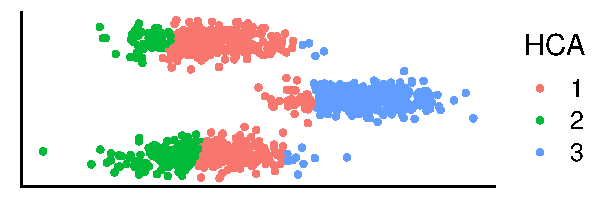
\includegraphics[width=2in]{Mahalanobis/img/hca.pdf}\quad%
	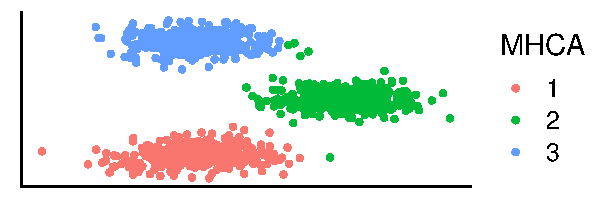
\includegraphics[width=2in]{Mahalanobis/img/mhca.pdf}
	\caption{Mahalanobis-based clustering (MHCA, right) captures the prolonged ellipsoid clusters better than commonly used hierarchical clustering (HCA, left)}
	\label{fig:mahaclust}
\end{figure}

\subsection{Contributions and Outline}

In the domain of clustering, algorithm performance has often been successfully improved by proper reimplementation for GPU hardware accelerators~\cite{krulivs2020detailed,gowanlock2017clustering,cuomo2019gpu}.
However, the computation of the MHCA is relatively irregular and rather complex, making the usual acceleration approaches ineffective.

As the main contribution of this paper, we describe our adaptation of MHCA for contemporary GPUs.
In particular, we describe a data structure that can be used to accelerate HCA algorithms on GPUs in general, and provide additional insight about efficiency of the specific parts of MHCA algorithm.
We subjected the implementation to comprehensive experimental evaluation and compared it with the existing implementation of MHCA to measure the achieved speedup.
Finally, we made the implementation available as open-source\footnote{\url{https://github.com/asmelko/gmhc}}, making it useful for both biological research and further experiments with parallelization of HCAs.

The mathematical and algorithmic overview of MHCA clustering is presented in Section~\ref{sec:mhca}, Section~\ref{sec:implementation} describes our proposed GPU implementation. We summarize the experimental evaluation in Section~\ref{sec:experiments}. Section~\ref{sec:relwork} puts the our research in proper context with prior work and Section~\ref{sec:conclusions} concludes the paper.


\section{Hierarchical Clustering with Mahalanobis Distance}\label{sec:mhca}
\label{sec:maha}

In this section, we review the necessary formalism and show the Mahalanobis average-linked hierarchical clustering algorithm.
The input dataset is a set of points in $d$-dimensional vector space, here assumed in $\mathbb{R}^d$, which is a common representation for cytometry data~\cite{shapiro2005practical}.
The algorithm produces a binary tree of \emph{clusters} where each resulting cluster is a subset of the input dataset of highly similar (`close' by some metric in the vector space) points.

Mahalanobis distance~\cite{mahalanobis1936generalized} is defined between a point $x$ and a non-singleton set of compact points $P$ as
\[ \delta_M(x,P) = \sqrt{(x-\bar{P})^T(\cov P)^{-1}(x-\bar{P})}, \]
where $\bar{P}$ is the centroid (mean) of the set $P$, and the entries of the covariance matrix are computed as
\[ (\cov P)_{ij} = \left(|P|-1\right)^{-1}\cdot \sum_{p \in P}{(p_i - \bar{P}_i)\cdot(p_j - \bar{P}_j)}. \]

One can intuitively view Mahalanobis distance as an Euclidean distance from the cluster centroid that also reflects the shape and the size of the cluster.
In particular, in a space that has been linearly transformed so that the covariance matrix of the cluster is a unit matrix, Euclidean and Mahalanobis distance coincide, as shown in Figure~\ref{fig:maha}.

\begin{figure}[t]
\centering
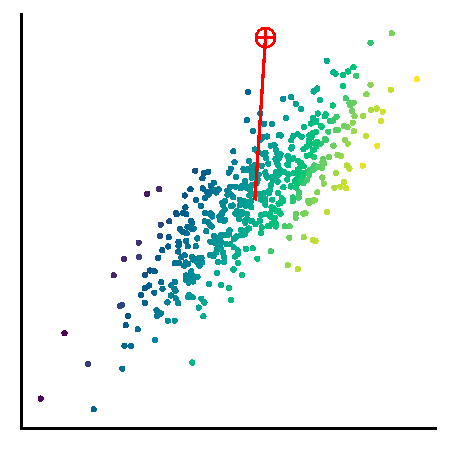
\includegraphics[width=1in]{Mahalanobis/img/maha1.pdf}\quad%
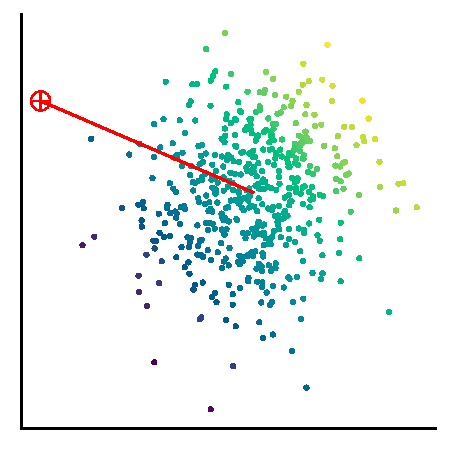
\includegraphics[width=1in]{Mahalanobis/img/maha2.pdf}
\caption{Mahalanobis distance (left) can be perceived as Euclidean distance (right) in a linearly transformed space where the cluster is perfectly `round'.
}
\label{fig:maha}
\end{figure}

The MHCA algorithm can be described in steps as follows:
\begin{enumerate}
	\item \emph{Initialization}: Construct an `active set' of numbered clusters $P_{1,2,\dots,n}$, each comprising one input element (data point) as $P_i=\{e_i\}$ for each $i \in \{1\ldots n\}$ where $\{e_1,\dots,e_n\}$ denotes the input dataset.
	\item \emph{Iteration}: Until the active set contains only a single item, repeat the following:

	\begin{enumerate}
		\item Compute pairwise dissimilarities of all clusters in $A$, select the pair $(P_r, P_s)$ with lowest dissimilarity. Output pair $(r,s)$.
		\item Update the active set by removing $P_r, P_s$ and adding $P_{n+i} = P_r\cup P_s$, where $i>0$ is an iteration number.
	\end{enumerate}

	\item \emph{Result}: the binary tree is specified by the trace of $n-1$ pairs $(r,s)$.
\end{enumerate}

Properties of the output depend mainly on the exact definition of the dissimilarity function used in step 2.a.
The common choices include the common `single' linkage (minimum pairwise distance between the 2 points in different clusters), `complete' linkage (maximum distance), `average' linkage (mean distance across clusters), `centroid' linkage (distance of cluster centroids), and others.
The used distance is usually a metric in the vector space, such as Euclidean.
The choice of the dissimilarity calculation methods is critical for obtaining results suitable for given analysis; the available methods have been therefore been subjected to much optimization~\cite{shirkhorshidi2015comparison}.

\subsection{Mahalanobis dissimilarity}

Fišer et al.~\cite{fivser2012detection} proposed the \emph{full Mahalanobis distance} as a dissimilarity function for HCA as an average of all Mahalanobis distances across clusters, as $\text{FMD}(P_i, P_j) = (|P_i|+|P_j|)^{-1} \left(\sum_k \delta_M((P_i)_k, P_j) + \sum_k\delta_M((P_j)_k, P_i)\right)$.
While this construction is intuitively correct and allows the clustering to precisely capture various dataset phenomena that are common in cytometry, the definition opens many inefficiencies and border cases that need to be resolved:

\begin{itemize}
	\item Mahalanobis distance may be undefined for small clusters because the covariance matrix is singular or nearly-singular. This can be resolved by a complete or partial fallback to robust distance measures, as detailed in Section~\ref{sec:maho-singular}.
	\item Because the Mahalanobis distance of a fixed point to a cluster \emph{decreases} when the cluster size increases (e.g., as a result of being merged with another cluster), the minimal dissimilarity selected in the step 3 of the algorithm may sometimes be smaller than the previously selected one.
  A correction is thus needed to keep the dissimilarity sequence properly monotonic, giving uncluttered, interpretable dendrogram display~\cite{everitt2002cambridge}.
	\item The amount of required computation is significantly higher than with the other linkages (dissimilarity functions), requiring additional operations for computing the inverted covariance matrix and covariance-scaled Euclidean distances.
  We mitigate this problem by massive parallelization with GPU accelerators, as detailed in Section~\ref{sec:implementation}.
\end{itemize}

The computation of the `full' average Manalanobis distance is unavoidably demanding, requiring many matrix-vector multiplications to compute distances between all points of one cluster and the opposite cluster.
Following the variations of Euclidean dissimilarity measures for HCA, a \emph{centroid-based Mahalanobis distance} may be specified to use only the average of the distance to the centroids of the other cluster, as $\text{CMD}(P_i, P_j) = \frac{1}{2} \left(\delta_M(\bar{P_i}, P_j) + \delta_M(\bar{P_j}, P_i)\right)$.
The result may be viewed as a fast approximate substitute for the full variant because the simplification removes a significant portion of the computational overhead and still produces sound results in many cases.
The difference between CMD and FMD is highly pronounced only when the centroids of the clusters are near, but their respective covariances differ, as visualized in Figure~\ref{fig:maha_var}.
Fortunately, such situations are quite rare in clustering of realistic datasets.

\begin{figure}[t]
  \centering
	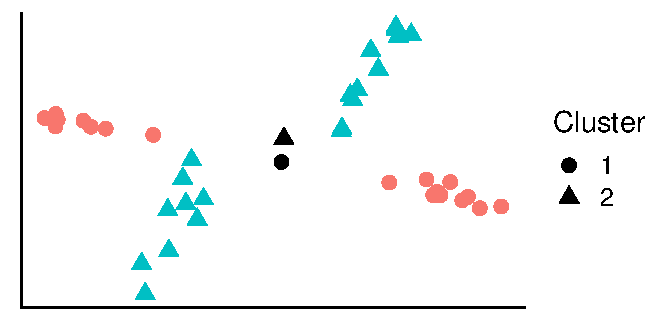
\includegraphics[width=2.2in]{Mahalanobis/img/dists.pdf}
	\caption{An example of two clusters for which the CMD fails to satisfactorily approximate the FMD (centroids are plotted in black).}
	\label{fig:maha_var}
\end{figure}

\subsection{Singularity of cluster covariance matrix}\label{sec:maho-singular}

In early iterations of MHCA, the clusters consist of only a few points.
Covariance matrix of a small cluster is likely singular, which means it is impossible to compute its inverse required by the Mahalanobis distance measure.
Furthermore, even for more points the covariance matrix may be nearly singular, and using its ill-conditioned inverse will yield inaccurate results and numeric floating-point anomalies (such as negative distances or infinities).

To solve this problem, Fišer et al.~\cite{fivser2012detection} proposed the following approach:
If the number of elements in a cluster relative to whole dataset size is lower than a threshold, the covariance matrix of such cluster is transformed so it can be inverted, and handled in a numerically safe manner.
We will denote the used threshold as the \emph{Mahalanobis threshold}, and categorize the clusters as \emph{sub-threshold} and \emph{super-threshold cluster}, depending on their size being below and above the Mahalanobis threshold respectively.

We later explore the following \emph{subthreshold handling methods} for managing the problematic covariance matrix values:
\begin{itemize}
	\item \textsc{Mahal} smoothly pushes the vectors of the covariance matrices of the sub-threshold clusters towards a unit sphere, so that the space around the clusters is not excessively distorted (or projected).
	\item \textsc{EuclidMahal} enforces unit (spherical) covariance vectors of the sub-thres\-hold clusters (thus enforcing Euclidean distances).
    Despite the simplicity and effectiveness, the hard thresholding may lead to a non-intuitive behavior; for example, the merging of a pair of large elliptical clusters that are just above the threshold may be prioritized over a pair of more similar but sub-threshold clusters.
	\item \textsc{Euclid} enforces unit covariances of all clusters \emph{only until the last sub-threshold cluster is merged}.
    This option usually leads to a viable formation of compact clusters, but completely ignores the possible intrinsic structure of several super-threshold clusters.
\end{itemize}

\subsection{Complexity and parallelization opportunities of MHCA}

A straightforward serial implementation of MHCA (such as the implementation in \texttt{mhca} R package\footnote{\url{https://rdrr.io/github/tsieger/mhca}}) works with iterative updates of the dissimilarity matrix.
Let us examine in detail the time complexity of the individual algorithm steps on a dataset that contains $n$ points of $d$ dimensions:

First, the algorithm constructs a dissimilarity matrix in $\mathcal{O}(d\cdot n^2)$, and identifies the most similar cluster pair in $\mathcal{O}(n^2)$. Then a total of $n-1$ iterations is performed as such:
\begin{itemize}
  \item a covariance matrix of the merged cluster is computed ($\mathcal{O}(d^2\cdot n)$) and inverted ($\mathcal{O}(d^3)$),
  \item the dissimilarity matrix is updated ($\mathcal{O}(d^2\cdot n)$), and
  \item the new most similar cluster pair is identified ($\mathcal{O}(n^2)$).
\end{itemize}

The total complexity is thus $\mathcal{O}(d\cdot n^2 + (n-1) \cdot (d^2\cdot n + d^3 + n^2))$.
Assuming $d\ll n$, the asymptotic complexity can be simplified to $\mathcal{O}(n^3)$.
Since we cache the unchanged dissimilarity matrix entries, the memory complexity is $\mathcal{O}(n^2)$.

In an idealized parallel execution environment (PRAM model with concurrent reads and infinite parallelism), we could improve the algorithm to perform faster as follows:
All cluster dissimilarity computations (including the later dissimilarity matrix update) can be performed in parallel in $\mathcal{O}{(d^3\cdot \log n)}$, using parallel reduction algorithm for computing the covariance sums.
The most similar cluster pair can be selected using a parallel reduction over the dissimilarity matrix in $\mathcal{O}(\log^2 n)$.
The total required time would thus be reduced to $\mathcal{O}(d^3 n\log^2 n)$ (again assuming $d\ll n$), using $\mathcal{O}(n^2)$ memory.

While this suggests two main ways of performance improvement for the massively parallel GPU implementation, the specifics of the current GPUs pose problems for such naive parallelization approach:
\begin{itemize}
	\item Parallelization of any single covariance matrix computation will improve performance only if the covariance matrix is sufficiently large, otherwise the performance may be reduced by scheduling overhead and limited parallelism.
	\item Scanning of the large dissimilarity matrix is parallelizable, but is hindered by relatively small amount of available GPU memory and insufficient memory throughput.
\end{itemize}

In the following section, we address these problems with optimizations that make the computation viable on the modern accelerators.
In particular, we show that the computation of a covariance matrix can be divided into many independent parts, thus exposing sufficient parallelization opportunities, and we demonstrate a technique for efficient caching of intermediate contents of the dissimilarity matrix to reduce the memory footprint and throughput requirements of the algorithm.

% -----------------------------------------------------------------------------
\section{GPU Implementation}\label{sec:implementation}
% -----------------------------------------------------------------------------

Memory handling optimizations form the essential part of our GPU implementation of MHCA, here called \emph{GMHC} for brevity.
Most importantly, we address the tremendous memory requirement of storing the dissimilarity matrix ($\mathcal{O}(n^2)$) for large $n$.
We replace this matrix with a special \emph{nearest-neighbor array}, which provides similar caching benefits, but requires only $\mathcal{O}(n)$ memory.
This saving in memory volume is redeemed by a slightly higher computational complexity; however, the measured improvement in scalability warrants this trade-off.

\begin{defn}[Nearest neighbor array]
	For clusters $P_1,\dots,P_n$ and a symmetric dissimilarity function $d$, the \emph{nearest neighbor array} $N$ contains $n-1$ elements defined as
	\[N_i = \argmin_{j>i} d(P_i,P_j).\]
	\label{def:nna}
\end{defn}

%(Symmetricity of $d$ is required to reduce the scope of $\argmin$ from original $j\neq i$.)

Maintaining a nearest neighbor array in the HCA computation allows us to reduce the amount of distance computations performed after each update.
In particular, when a cluster pair $(P_i,P_j)$ is merged into new cluster $P_m$, only elements with values $i$ and $j$ have to be recomputed, along with the new value for $N_m$

This is enabled by the symmetry of $d$, which allowed us to ensure that the contents of the nearest neighbor arrays at some index \emph{only depend on clusters with higher indices}.
If we set the new index $m$ to be smaller than all existing indices in the array (i.e., $m=1$, shifting the rest of the array), the newly appearing cluster can not invalidate the cached indices for the original array, and only the entries that refer to the disappearing clusters $i,j$ need to be recomputed.
In consequence, if an already present cluster $P_k$ was to form the most similar pair with the new cluster $P_m$, this information would be present the $\argmin_{k>m}$ computation, and stored in $N_m$ instead of $N_k$.

In an optimistic scenario, the above optimization can be used to limit the number of elements that need to be updated in each iteration by a constant number, which leads to a major increase in overall performance.
This constant limit is supported by empirical observations on realistic datasets with around 1 million of objects, where the number of triggered updates was rarely over $50$.
Further, we reduce the need for recomputation by caching several `nearest' neighbors for each entry of $N$:

\begin{defn}[Neighbor buffer]
A sorted list of $L$ nearest neighbor indices (respectively to the $\argmin_{j>i}$ in definition~\ref{def:nna}) stored for each item in $N$ is called a \emph{neighbor buffer}.
\end{defn}

To ensure the efficiency of the process, we split the update of neighbor buffers to two parts:
First, when $(P_i,P_j)$ is merged into $P_m$, all buffers are filtered and values $i$ and $j$ are removed (i.e, replaced with dummy values).
On recomputation, all empty buffers (including newly formed $N_m$) are filled with indices of nearest $L$ neighbors, while the partially filled buffers are left intact.
This allows us to reuse the intermediate results of the computation of an $N$ array entry for as much as $L$ recomputations that involve the cluster.

The complexity of updating the nearest neighbor array element $i$ for the neighbor buffer of size $L$ on $m$ clusters, using a pair dissimilarity computation of complexity $\mathcal{O}(\delta)$, is $\mathcal{O}((m-i)\cdot (\delta+L))$.
The reduced amount of index updates thus trades off for index update complexity, depending on $L$.
The optimal choice of $L$ is discussed later in Section~\ref{sec:exp}.

\subsection{Algorithm overview}

The hierarchical clustering of $n$ initial clusters is a series of $n-1$ iterations, such that in each iteration two clusters are merged into one. Before the first iteration, the nearest neighbor array $N$ must be initialized.
Each subsequent iteration comprises the following compact steps:
\begin{enumerate}
	\item Scan the neighbor array and fetch the most similar cluster pair
	\item Create a new cluster by merging the cluster pair
	      \subitem Compute its corresponding centroid and covariance matrix
	      \subitem Transform and invert the covariance matrix
	\item Update the neighbor array (only required if $n\geq 3$)
\end{enumerate}

\begin{figure}[t]
\centering
	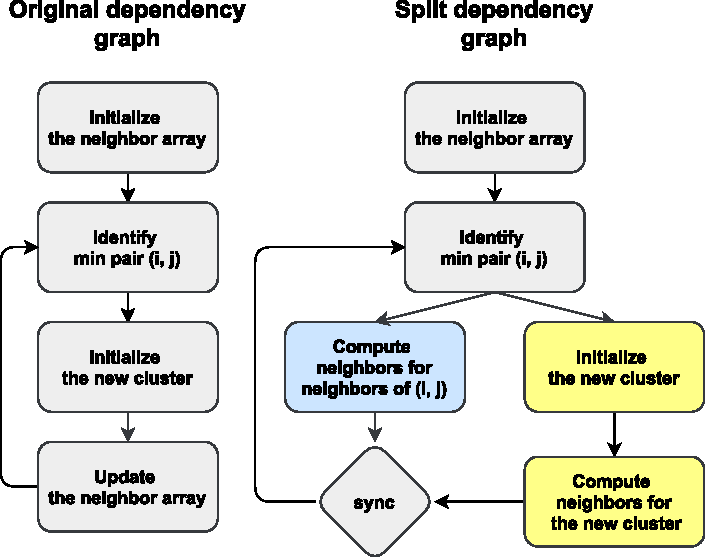
\includegraphics[width=8cm]{Mahalanobis/img/dependency-graph}
	\caption{The original graph of dependencies and the proposed split dependency graph, where blue and yellow boxes can be executed concurrently}
	\label{fig:dep-graph}
\end{figure}

The individual parts of the algorithm may be scheduled and executed dynamically, ordered only the data dependencies as displayed in Figure~\ref{fig:dep-graph}.
Mainly, this allows us to split the update of the neighbor array into update of the neighbors of old clusters ($i$, $j$) and the update of the newly created cluster.
Naturally, the individual steps are internally implemented as data-parallel operations as well.

In GMHC, we control the iteration loop from the host code, while the work of each update step is implemented within a CUDA kernel.
Our code employs CUDA streams~\cite{cuda} to efficiently implement the execution overlaps, creating some high-level task parallelism in the process.
In the rest of this section, we detail the implementations of the individual CUDA kernels.


\subsection{Cluster merging and covariance computation}

Covariance matrix $\cov P$ of cluster $P$ (and its inversion) is computed only when a cluster is formed; in our case when two clusters are merged.
In GMHC, we iterate over all data points $x \in P$ and each item $(\cov P)_{ij}$ is computed as a sum of centered products of $x_i$ and $x_j$ (following the definition from Section~\ref{sec:maha}).
As the most pressing issue, the performance of this process depends on fast finding of data points $x$ that belong to the cluster in the array of all data points.

A possible straightforward solution, storing an array of assigned points for each data cluster so that the assigned points can be accessed in a fast and compact way, would require dynamic memory allocation or manual apriori over-allocation, and many data moving operations.
We settled for a more compact solution with an assignment array that stores a cluster indices for each data point.
Although that does not require data copying, both the cluster merge and the retrieval of one cluster points will take $\mathcal{O}(n)$ time.
Fortunately, the two operations can be performed by a single parallel scan of the assignment array in this case.

\subsubsection{Covariance kernel implementation.}

The covariance kernel takes advantage of the symmetry of a covariance matrix and computes only its upper triangle.
Additionally, extra parallelism can be obtained by slicing the computation of the covariance matrix from Section~\ref{sec:maha} over individual data point contributions $\mathbf{S}^x$, as
$\cov P = (|P|-1)^{-1}\sum_{x\in P}\mathbf{S}^x$, where
$\mathbf{S}^x_{ij}=(x_i-\mathbf{\bar{x}}_i)\cdot(x_j-\mathbf{\bar{x}}_j)$.

The kernel is implemented as a loop over all data points.
A whole CUDA warp is assigned one data point and computes the intermediate $\mathbf{S}^x$.
These are then added together in a two-step reduction --- all intermediate states within a CUDA block are reduced using shared memory, which is then followed by a global reduction performed by a separate kernel launch that outputs the totals in a single covariance matrix.

Notably, the covariance matrices of single-point clusters are not computed; rather, they are assigned a default unit matrix.

\subsection{Inverse covariance storage optimization}
\label{subsec:icov}

The Mahalanobis distance requires inversion of the covariance matrix, which needs to be computed from the results of the previous step.
We use \texttt{cuSolver} library\footnote{\url{https://docs.nvidia.com/cuda/cusolver/index.html}} for implementing the matrix inversion, namely the routines \texttt{potrf} and \texttt{potri}.

The inverted matrix is subsequently transformed to better suit the Mahalanobis distance formula, and to eliminate redundant computations later in the process. In particular, we rewrite the Mahalanobis formula for inverse covariance matrix $M$ as a quadratic form
\[x^T M x =
  \sum_{i=1}^{d}\sum_{j=1}^{d}m_{ij}x_ix_j = \sum_{i=1}^{d}m_{ii}x_i^2 + \sum_{i=1}^{d}\sum_{j>i}^{d}2m_{ij}x_ix_j,\]
allowing us to store only the upper-triangular part of the matrix, pre-multiplied by $2$.

\subsection{Maintenance of nearest neighbor array}

GMHC implements 2 similar processes for the neighbor array initialization and update, differing mainly in the granularity of the task size.
We thus only focus on the update implementation.

First, specific simplified version of kernel for computing the distances is used for cases when the covariance matrix is unit, falling back to efficient implementation of Euclidean distance.
The decision which kernel to execute is done in the host code, depending solely on the selected subthreshold handling method (explained in Section~\ref{sec:maho-singular}) and the size of the two involved clusters.
The decision is formalized in Table~\ref{tab:neigh-select}.

\begin{table}[b]
	\centering
	%\setlength{\tabcolsep}{10pt}
	\begin{tabular}{@{}llll@{}}
		\toprule
		Subthreshold handling method~~ & sub/sub~~ & sub/super~~ & super/super \\
		\midrule
		\textsc{Euclid}      & \texttt{euclid} & \texttt{euclid} & \texttt{maha}  \\
		\textsc{EuclidMahal} & \texttt{euclid} & \texttt{maha}   & \texttt{maha}  \\
		\textsc{Mahal}       & \texttt{maha}   & \texttt{maha}   & \texttt{maha}  \\
		\bottomrule
	\end{tabular}
  \smallskip
	\caption{The host-side selection of the neighbor-distance kernel}
	\label{tab:neigh-select}
\end{table}


\subsubsection{The neighbor array update kernel.}

The update operation of nearest neighbor buffer array entry $N_i$ is defined as finding $L$ nearest clusters with index greater than $i$, and storing their ordered indices into $N_i$ neighbor buffer.
We split this operation in two parts, each handled by a separate kernel:
\begin{enumerate}
	\item Compute distances between all relevant cluster pairs concurrently.
	\item Reduce the results into a single nearest neighbor buffer entry.
\end{enumerate}

The execution of the first step differs between the Euclidean and the Mahalanobis neighbor computation.
While the former parallelizes trivially with one thread computing one distance value, the complex computation of Mahalanobis distance executes faster if the whole warp cooperates in one distance computation.

The precise operation needed to compute the Mahalanobis distance is a vector-matrix-vector multiplication.
To evaluate the formula from Section~\ref{subsec:icov}, we utilize the fuse-multiply-add intrinsic instructions to accumulate the results of the assigned work into their privatized buffers, which are subsequently reduced using fast warp-shuffle instructions.

In the second step, which selects the nearest $L$ indices, is the same for both distance measures.
We use a three-level implementation:
At the first level, the threads accumulate local minima of small array slices into their registers.
At the second level, each thread block utilizes the shared memory to efficiently exchange data and compute block-wise minima.
The third level collects the resulting minima and performs the same final reduction on a single thread block (thus efficiently utilizing intra-block synchronization).
The second and the third level could be fused together if the atomic instructions were used to synchronize data updates explicitly; however, we observed the improvement was negligible and preferred to reduce the design complexity instead.

This whole neighbor buffer `refill' operation is performed concurrently for every index in the nearest neighbor array that needs to be updated.
Our implementation executes a separate CUDA grid for each update, which reduces implementation complexity but still allows the grids to run concurrently and utilize the entire GPU.


% -----------------------------------------------------------------------------
\section{Experimental Results}\label{sec:experiments}
% -----------------------------------------------------------------------------

We have subjected our implementation of GMHC to extensive experimental evaluation, measuring the effect of main design choices in the algorithm.
In this section, we present the most important results and we put them in proper context, particularly with respect to parameter selection and scaling.

\subsection{Benchmarking methodology and datasets}

The experiments were performed on two systems --- a high-end server equipped with NVIDIA Tesla V100 SXM2 (32 GB) and a mainstream PC with NVIDIA GeForce GTX 980 (4 GB).
Both systems used Linux CentOS 8 with CUDA Toolkit (11.2).

We used the original MHCA clustering implementation by Fišer et al.~\cite{fivser2012detection} as a baseline, which is, to our best knowledge, the only other publicly available MHCA implementation.
The baseline algorithm is written in C as strictly sequential without explicit utilization of SIMD instructions; but it properly utilizes the highly-optimized \texttt{Blas} library for most heavy computation.
It was benchmarked on a high-end server with Intel Xeon Gold 5218 CPU, clocked at $2.3$~GHz (with 64 logical cores) and $384$~GB RAM (the same as the high-end server used for benchmarking GMHC).
We stress that the comparison between CPU and GPU implementation is not entirely objective, and the test results should be perceived more as a measure of overall data capacity improvement than of the implementation quality.
We did not test MHCA on the mainstream PC platform, because of the enormous $\mathcal{O}(n^2)$ memory requirements totaled to hundreds of gigabytes in our benchmarks.

As testing data, we used several high-dimensional datasets originating in mass cytometry~\cite{weber2016comparison}, namely the \texttt{Nilsson\_rare} (44K data points, 14 dimensions), \texttt{Levine\_32dim} (265K data points, 32 dimensions) and \texttt{Mosmann\_rare} (400k data points, 15 dimensions).
For brevity, we report only a subset of the measured results, but these should generalize well to other data.
In particular, we did not observe any significant data-dependent performance differences.

In all experiments, we measured the wall time of the total algorithm execution.
The experiments were performed multiple times to prevent random deviations in measurement; we display mean values of the measurements.
Because the experimental evaluations on both mentioned GPUs behaved consistently with no surprising differences on any particular hardware, we present mainly the results from Tesla V100 SXM2 GPU unless stated otherwise.

\subsection{Experiment results}\label{sec:exp}

First, we evaluated the scalability of the GMHC implementation depending on the size of the dataset.
The inputs of different sizes were achieved by randomly sub-sampling the Mosmann dataset.
Figure~\ref{fig:perf_methods} shows the wall time for each subthreshold method, revealing that the performance scales sub-quadratically with data size.
Notably, the optimized implementations of \textsc{Euclid} and \textsc{EuclidMahal} scale about $10\times$ better than full \textsc{Mahal} for this dimensionality.

\begin{figure}[t]
	\centering
	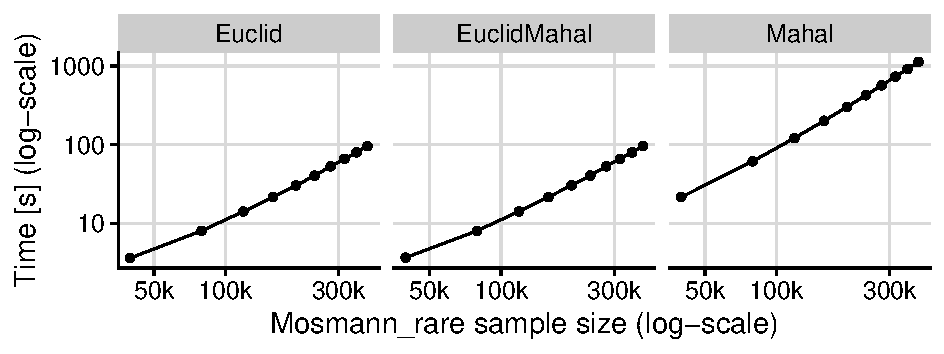
\includegraphics[width=8cm]{Mahalanobis/img/methods.pdf}
	\caption{Comparison of the subthreshold distance computation method performance.}
	\label{fig:perf_methods}
\end{figure}

The tradeoff between Euclidean and Mahalanobis computation in the first two methods can be further controlled by setting the threshold value $t$, controlling whether a cluster is considered small or large, and in turn, deciding the dissimilarity metric to use.
Figure~\ref{fig:perf_thresh} summarizes the performance gains for various setting of this threshold.

\begin{figure}[t]
	\centering
	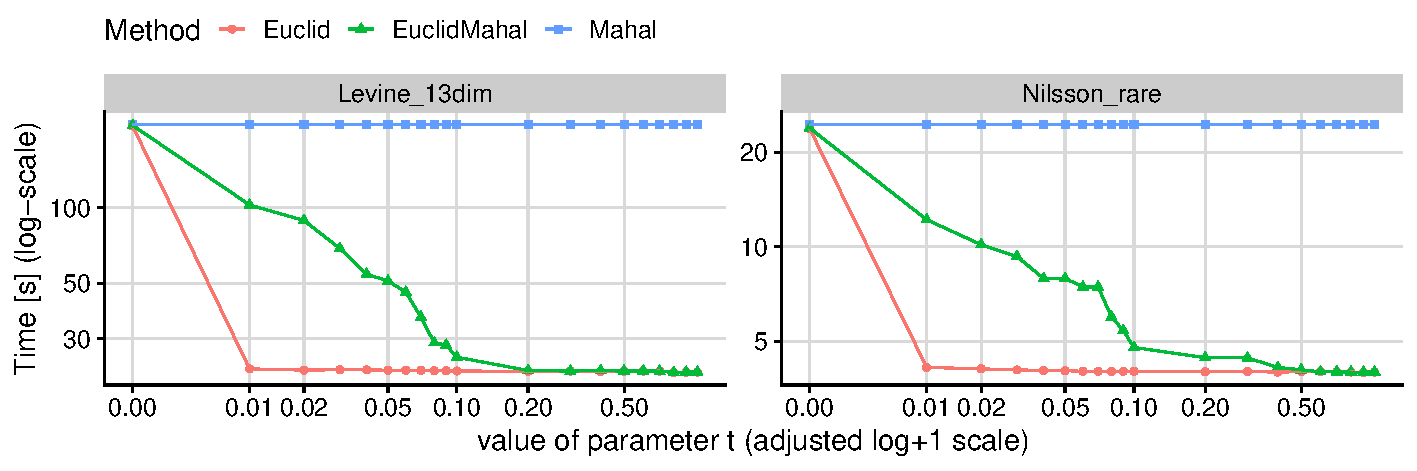
\includegraphics[width=12cm]{Mahalanobis/img/thresh.pdf}
	\caption{Clustering time of subthreshold methods with varying Mahalanobis threshold value on two different datasets.}
	\label{fig:perf_thresh}
\end{figure}

In the figure, $t=0$ forces all methods perform dissimilarity measurements using the Mahalanobis distance. When we increase $t$ only very slightly to $0.01$, the \textsc{Euclid} method time decreases dramatically and stays almost the same in the remainder of $t$ range. This is often caused by small sub-threshold clusters that are propagated to the very end of the clustering, which postpones the switch to the Mahalanobis distance. On the other hand, the \textsc{EuclidMahal} method shifts its wall time smoothly towards the \textsc{Euclid} method as $t$ increases, which is a consequence of the first super-threshold cluster appearing later in the process.

To determine the optimal value of the nearest neighbor buffer size, we benchmarked the clustering of datasets with a range of parameters $L$ (Figure~\ref{fig:perf_nei}).

\begin{figure}[t]
	\centering
	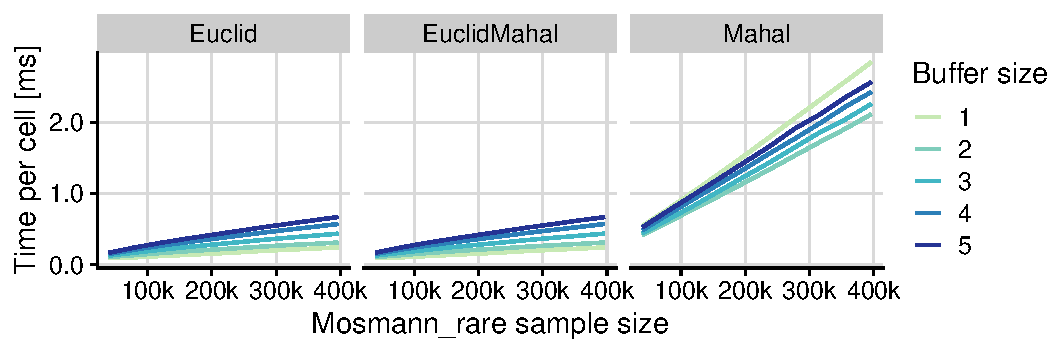
\includegraphics[width=9cm]{Mahalanobis/img/neighbors.pdf}
	\caption{Comparison of neighbor buffer sizes for subthreshold methods ($t=0.5$)}
	\label{fig:perf_nei}
\end{figure}

Curiously, the observed results show that while $L=1$ is optimal for \textsc{Euclid} and \textsc{EuclidMahal}, it performs worst for \textsc{Mahal} method. This is a consequence of the used distance function in dissimilarity measurements --- for the \textsc{Euclid} and \textsc{EuclidMahal} method, where the Euclidean distance function dominates, the time difference for performing smaller number of neighbor updates did not balance the increased time complexity of a single update. The \textsc{Mahal} method works optimally with $L=2$; as the $L$ increases further, the performance starts to decrease again. 

Similarly, the optimal value of $L$ increases for higher-dimensional datasets, which we tested on Levine\_32dim data (detailed results not shown). In particular, for Mahalanobis distance, we measured the same optimal value $L=2$ with much greater performance gain (over $30\%$) against $L=1$ than on the Mosmann dataset. We expect that the optimal value of $L$ will continue to increase with the dimensionality of the dataset in case of the \textsc{Mahal} method. On the other hand, the Euclidean-based methods kept their optimum at $L=1$.

\begin{figure}[t]
	\centering
	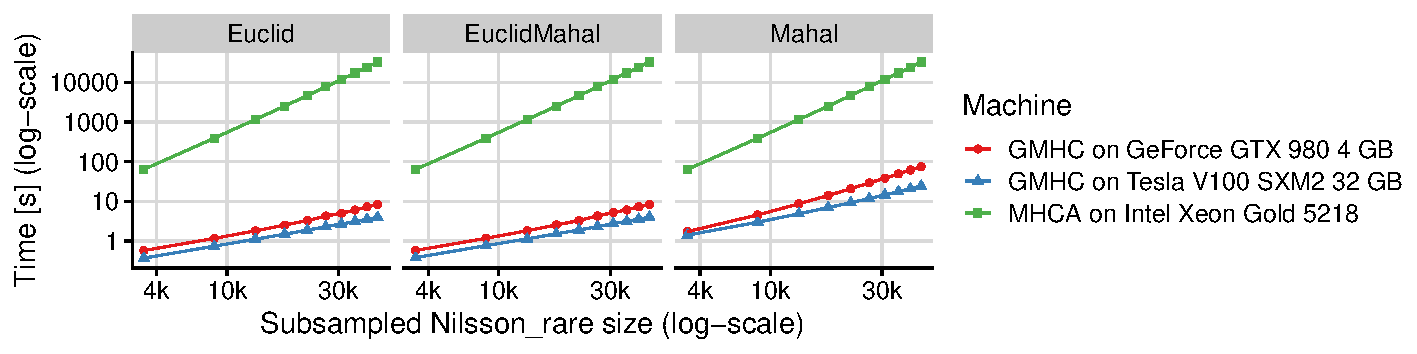
\includegraphics[width=12cm]{Mahalanobis/img/comparison.pdf}
	\caption{GMHC and MHCA comparison on Nilsson dataset with default $t=0.5$.}
	\label{fig:perf_comp}
\end{figure}

Finally, we compared the performance of GPU implementation of MHCA to the CPU baseline, to estimate the outcome for practical data analysis scalability.
Figure~\ref{fig:perf_comp}) indicates an overall performance increase by up to $1400\times$ in case of the \textsc{Mahal} method and by up to $8000\times$ in case of mixed-Euclidean methods.
When comparing performance on the older `gaming' GTX 980 GPU, the speedups were around $400\times$ and $4000\times$, respectively.
In summary, modern GPUs have been able to accelerate the MHCA task by more than three orders of magnitude, which is consistent with the effects of parallelization applied to many other clustering algorithms.


% -----------------------------------------------------------------------------
\section{Related Work}\label{sec:relwork}
% -----------------------------------------------------------------------------

The original version of MHCA clustering for flow cytometry by Fišer~et~al.~\cite{fivser2012detection} used a MATLAB implementation to analyze datasets of around $10^4$ multi-dimensional data points.
Due to the limited scalability and interoperability with modern data analysis environments, a C version of the algorithm has been implemented within R package \texttt{mhca} and enhanced with the possibility of assuming apriori clusters for approximation, to reduce the unfavorable $\mathcal{O}(n^3)$ time complexity for large datasets.
That allowed the authors to process datasets of around $10^6$ data points within an interactive environments~\cite{kratochvil2020shinysom}.

Despite of the performance advancement, the approximation in the method did not retain the sensitivity required to detect various small clusters of interest (i.e., small cell populations), such as the `minimum residual disease' cells crucial for diagnosis of acute myeloid leukemia~\cite{fivser2012detection}.
Similar approximations are used in many other clustering methods to gain performance at the cost of precision justifiable in a specific domain; including the 2-level meta-clustering approach of FlowSOM~\cite{gassen2015flowsom}, and advanced approximate neighborhood graph structure of FastPG~\cite{fastpg}.

Acceleration of HCAs on GPUs has been explored by several authors:
Chang et al.~\cite{chang2009hierarchical} discuss hierarchical clustering of gene mRNA levels assayable by DNA microarray technology.
Their GPU code computes matrix of pairwise distances between genes using Pearson correlation coefficient as one of the present metrics, and utilized a special property of data to effectively perform single-linkage over the present matrix.
Zhang et al.~\cite{zhang2006hierarchical} used similar clustering methodology, but employed GPU texture elements for the data representation of gene expression profile HCA.
Both acceleration methods resulted in performance increase between $5\times$ to $30\times$ on datasets of $10^4$ data points.


% -----------------------------------------------------------------------------
\section{Conclusions}\label{sec:conclusions}
% -----------------------------------------------------------------------------

We have presented an implementation approach for Mahalanobis-average linkage hierarchical clustering algorithm, which utilizes modern parallel GPU accelerators to increase its performance.
In the benchmarks, our GPU implementation GMHC has achieved over $10^3\times$ speedup on practical datasets over the current CPU implementations, which enabled scaling of the MHCA algorithm to large datasets produced by current data acquisition methods.

Together with the open-source implementation, we have provided a new high-performance building block for dataset analyses which should support the growing demand for fast data analysis methods not only in cytometry, but also in other areas of data analysis dealing with irregularly shaped Gaussian clusters.

The implementation structure detailed in the paper has allowed us to streamline the utilization of parallel hardware for accelerating general hierarchical clustering algorithms.
We expect that the proposed data structures will be ported to support acceleration of dissimilarity measures in other hierarchical clustering methods, providing a solid building block for future acceleration of data mining and knowledge discovery.


% \subsection*{Acknowledgements}

% This work was supported by Czech Science Foundation (GAČR) project 19-22071Y,
% by ELIXIR CZ LM2018131 (MEYS),
% by Charles University grant SVV-260451,
% and by Czech Health Research Council (AZV) [NV18-08-00385].



\chapter{Astute Approach to Handling Memory Layouts of Regular Data Structures}
% %
% \titlerunning{Handling Memory Layouts of Regular Data Structures}
% % If the paper title is too long for the running head, you can set
% % an abbreviated paper title here
% %
% \author{
%     % Anonymous\inst{1}
%     Adam Šmelko\inst{1} \and %
%     Martin Kruliš\inst{1} \and %
%     Miroslav Kratochvíl\inst{2} \and %
%     Jiří Klepl\inst{1} \and % https://orcid.org/0000-0002-2231-4073
%     Jiří Mayer\inst{1} \and % https://orcid.org/0000-0001-6503-3442
%     Petr Šimůnek\inst{1} %https://orcid.org/0000-0003-0089-7201
% }
% \authorrunning{
%     % Anonymous et al.
%     Šmelko et al.
% }
% % First names are abbreviated in the running head.
% % If there are more than two authors, 'et al.' is used.
% %
% \institute{
%     % Anonymized due to double-blind review process
%     Department of Distributed and Dependable Systems, Charles University, Prague, Czech Republic\\
%     \email{\{smelko,krulis\}@d3s.mff.cuni.cz}
%     \and
%     Luxembourg Centre for Systems Biomedicine, University of Luxembourg, Esch-sur-Alzette\\
%     \email{miroslav.kratochvil@uni.lu}
% }
% %
% \maketitle              % typeset the header of the contribution
% %
% \begin{abstract}
% Programmers of high-performance applications face many challenging aspects of contemporary hardware architectures. One of the critical aspects is the efficiency of memory operations which is affected not only by the hardware parameters such as memory throughput or cache latency but also by the data-access patterns, which may influence the utilization of the hardware, such as re-usability of the cached data or coalesced data transactions. Therefore, a performance of an algorithm can be highly impacted by the layout of its data structures or the order of data processing which may translate into a more or less optimal sequence of memory operations. These effects are even more pronounced on highly-parallel platforms, such as GPUs, which often employ specific execution models (lock-step) or memory models (shared memory).

% In this work, we propose a modern, astute approach for managing and implementing memory layouts with first-class structures that is very efficient and straightforward. This approach was implemented in \Noarr{}, a GPU-ready portable C++ library that utilizes generic programming, functional design, and compile-time computations to allow the programmer to specify and compose data structure layouts declaratively while minimizing the indexing and coding overhead. We describe the main principles on code examples and present a performance evaluation that verifies our claims regarding its efficiency.
% \keywords{memory layout \and data structure \and cache \and parallel \and performance \and reusable}
% \end{abstract}

% -----------------------------------------------------------------------------
\section{Introduction}
% -----------------------------------------------------------------------------

This paper aims to tackle memory-related performance issues, which represent one of the most crucial performance optimization topics. In hardware, memory access is optimized by providing faster memories closer to the chip (like HBM2), multi-level caches and transfer buffers, and even specialized explicit near-core memories (such as AVX512 registers or shared memory in Nvidia GPUs). Software developers benefit from these features by creating specialized, cache-aware algorithms, often tailored for a particular architecture.

The design of the way that the program data is laid out in memory is one of the crucial steps that ensures memory access performance. Even simple design choices like row- or column-major matrix storage impact the performance within the complex memory cache models by simplifying address translations, improving cache hit ratio and prefetching, or ensuring the alignment required for coalesced SIMD operations~\cite{clauss2000automatic,panda2001cache}. For parallel algorithms, the complexity of the problem becomes much broader because of cache-line collisions, false-sharing, non-uniform memory architectures, a variety of synchronization issues~\cite{bethel2015improving,heinecke2008parallel,weidendorfer2007latencies}, and other factors. Many-core platforms (GPUs in particular) only amplify this by enforcing specific data access patterns in lockstep execution, advocating the use of programmer-managed caches (like shared memory), and having a significantly lower cache-to-core ratio in comparison to the CPUs~\cite{guide2013cuda}.

The best layout is quite often elusive and needs to be discovered empirically. Furthermore, it often differs even among the utilized cache levels~\cite{weber2017matog,hawick2011hypercubic,krulivs2020detailed}. Consequently, the optimal implementations are often complicated, and most of the optimization-relevant code is not portable between hardware architectures. Enabling simple implementations of layout-flexible data structures and algorithms would improve the code portability (and value); however, systematic approaches are quite rare, often over-complicating the code logic and making the algorithm implementation not maintainable or usable beyond the community of specialists.


\subsection{Motivational example}

To explain the motivation, objectives, and contributions of our research, we have selected a matrix multiplication problem widely known in computer science. For the sake of simplicity, we use the most straightforward implementation with $\mathcal{O}(N^3)$ complexity (computing $C = A \times B$ of square matrices $N^2$):

\begin{minted}[fontsize=\scriptsize]{c++}
    for (size_t i = 0; i < N; ++i)
        for (size_t j = 0; j < N; ++j) {
            C[i][j] = 0;
            for (size_t k = 0; k < N; ++k)
                C[i][j] += A[i][k] * B[k][j];
        }
\end{minted}

Having a fixed algorithm structure (i.e., order of the operations), the memory layout of the matrices is the main issue affecting the performance. In this context, the layout is defined by transforming the abstract indices ($i,j$) into an offset, subsequently used to compute the actual memory address. For instance, the most common matrix layout is row-major, which computes the offset as $i*W + j$ (where $W$ is the width of the matrix). A few examples of possible layouts are depicted in Figure~\ref{fig:layout}.

\begin{figure}
    \begin{subfigure}{.19\textwidth}
        \centering
        \includegraphics[width=.9\linewidth]{noarr/figures/matrix-row-major}
        \caption{row-major}
        \label{fig:layout-row}
    \end{subfigure} 
    \begin{subfigure}{.19\textwidth}
        \centering
        \includegraphics[width=.9\linewidth]{noarr/figures/matrix-col-major}
        \caption{col-major}
        \label{fig:layout-col}
    \end{subfigure}
    \begin{subfigure}{.19\textwidth}
        \centering
        \includegraphics[width=.9\linewidth]{noarr/figures/matrix-tiled}
        \caption{row-tiles}
        \label{fig:layout-tile}
    \end{subfigure}
    \begin{subfigure}{.19\textwidth}
        \centering
        \includegraphics[width=.9\linewidth]{noarr/figures/matrix-zcurve}
        \caption{z-curve}
        \label{fig:layout-zcurve}
    \end{subfigure}
    \begin{subfigure}{.19\textwidth}
        \centering
        \includegraphics[width=.9\linewidth]{noarr/figures/matrix-hcurve}
        \caption{Hilbert curve}
        \label{fig:layout-hcurve}
    \end{subfigure}
    
    \caption{Examples of common matrix layouts}
    \label{fig:layout}
    \vspace{-10pt}
\end{figure}

The aforementioned code sample used traditional C notation \mintinline{c++}{A[i][j]} which enforces the row-major layout, which is sub-optimal for this algorithm. Having the second matrix in a col-major layout or using a z-curve for all matrices will improve cache utilization, and the algorithm would run several times to several orders of magnitude faster, depending on the platform. Therefore, we need to introduce layout flexibility into the code.

A typical object-oriented solution would be to create a class abstraction that would define a uniform interface for accessing matrix elements whilst enabling different implementations through derived classes. A slightly better and more reusable solution would be to separate the offset computation into a policy class that would be injected into the matrix as a template parameter:

\begin{minted}[fontsize=\scriptsize]{c++}
    class RowMajor {
        static size_t offset(size_t i, size_t j, size_t W, size_t H) {
            return i*W + j;  
        }
    };

    template<typename T = float, class Layout = RowMajor>
    class Matrix {
        /* ... */
        T& at(size_t i, size_t j) {
            return _data[Layout::offset(i, j, _W, _H)];
        }
    };
\end{minted}
  
The policy class makes the matrix implementation flexible (in terms of selecting the proper layout) and efficient (since the compiler can inline the static method). However, several drawbacks make this solution imperfect. The interface between the \texttt{Matrix} class and its layout policy (\texttt{RowMajor}) is created ad-hoc by the author of the main class, which complicates the code reusability of the layout policies in potentially compatible situations. The interface also prevents efficient constant propagation and caching of intermediate values. Furthermore, the strong encapsulation may prevent low-level optimizations, portability to other architectures (e.g., GPUs), and complicate data structure composition (e.g., when matrices in an array need to be interleaved).

We aim to design a more straightforward, more programmer-friendly solution to implementing \emph{layout-agnostic} algorithms, focusing on enabling performance optimizations and parallel processing.


\subsection{Objectives and contributions}

Our main objective was to create a library that allows the users to quickly adapt their algorithms and data structures for different memory layouts, with a~particular focus on the following targets:

\begin{itemize}
    \item Once an algorithm is adapted, it becomes layout-agnostic --- i.e., no subsequent internal code modifications should be required to change the layout of the underlying data structures.
    \item The layout representation should not be coupled with memory allocation so that it could be used in different scenarios and different memory spaces (i.e., directly applicable with memory-mapped files or GPU unified memory).
    \item The interface should define an easily comprehensible abstraction for \emph{indexing} (offset computation) that would hide its (possibly complex) nuances.
    \item The indexing mechanism should enable the compiler to evaluate constant expressions at compile time (e.g., fold constant dimensions of a structure into the generated code).
    \item The code overhead should be minimal, preferably smaller than with well-established practices, such as providing template policy classes to govern layout or allocation.
\end{itemize}

We have implemented \Noarr{} header-only library\footnote{\Noarr{} is available as open-source on GitHub under MIT license: \url{https://github.com/ParaCoToUl/noarr-structures}} for C++ as a prototype that achieves the outlined objectives. C++ was chosen as a widely-used mainstream language that provides complete control over memory layout and allocation and is widely used for programming performance-critical applications, including parallel HPC systems and GPGPU computing. Its fundamental features, like the templating system and operator overloading, open possibilities for generic programming, compile-time optimizations, and the design of a functional-like interface, which simplifies the use of the library. Furthermore, the separation of indexing from (CPU-specific) memory management allowed us to directly utilize the library with Nvidia CUDA code, easily porting the layout-agnostic code on contemporary GPUs.

We believe that \Noarr{} will make a significant contribution to simplifying the coding process and increasing performance in many scenarios, especially:
\begin{itemize}
    \item Empirical exploration of possible layouts --- i.e., finding the optimal combination of layouts for given data structures and algorithms by measuring the performance of all possible implementations.
    \item Implementing applications and libraries in which the optimal layout of data structures needs to be selected at runtime (e.g., based on the size of the problem or the best available architecture).
    \item Allowing simple yet efficient (semi)automatic layout transformations in case the input or output layouts differ from the optimal layouts for the computation.
\end{itemize}

Although the issues mentioned above can be identified in a large variety of data structures and algorithms, we are focusing mainly on regular data structures such as nested multi-dimensional arrays and structures (in the C/C++ sense). However, despite this narrow scope, we have identified that this problem is quite challenging, especially regarding optimizations for massively parallel environments like GPUs.

% Furthermore, \Noarr{} library enables research of semi-automated or automated selection of the best memory layout for given problem configuration, and automatic layout transformations of data structures that are often required when moving the data between memory types (e.g., when a row-major matrix from disk is transferred to a column-major format in memory). Here, we mainly demonstrate the possibility of automating the layout transformation process. Although the automated selection of the best data layouts for algorithms is easy to implement with the current version of \Noarr{}, a rigorous review of the methodology is well beyond the scope of this paper.


The paper is organized as follows. Section~\ref{sec:layouts} explains the key principles and benefits of the layout-agnostic algorithm design. The performance aspects of offset computation overhead are summarized in Section~\ref{sec:perf}. In Section~\ref{sec:implementation}, we provide insights into the current implementation of the \Noarr{} library. Related work and main conclusions are summarized in Sections~\ref{sec:relwork} and \ref{sec:conclusion}.

%\section{Motivational Example}\label{sec:motivation}

To demonstrate both performance- and programming-related aspects of the data layout reorganization, we selected a matrix data structure, which is well-known by all scientists and programmers. Matrix is two-dimensional regular array where the individual elements are simple scalars (e.g., floats) and there are many ways how it can be stored in linear memory.

The two most typical layouts are the \emph{row-major} and \emph{column-major} formats, where the items in each row (or column, respectively) form a continuous sequence. The memory offset of item at position $[i,j]$ is computed as $i\cdot W + j$ in row-major layout, and $j*H + i$ in column-major layout, where $i$ is a zero-based index of the row, $j$ is the index of the column, and $W,H$ stand for the width and the height of the matrix respectively.

\begin{figure}
\begin{subfigure}{.19\textwidth}
    \centering
    \includegraphics[width=.9\linewidth]{figures/matrix-row-major}
    \caption{row-major}
    \label{fig:layout-row}
\end{subfigure} 
\begin{subfigure}{.19\textwidth}
    \centering
    \includegraphics[width=.9\linewidth]{figures/matrix-col-major}
    \caption{col-major}
    \label{fig:layout-col}
\end{subfigure}
\begin{subfigure}{.19\textwidth}
    \centering
    \includegraphics[width=.9\linewidth]{figures/matrix-tiled}
    \caption{row-tiles}
    \label{fig:layout-tile}
\end{subfigure}
\begin{subfigure}{.19\textwidth}
    \centering
    \includegraphics[width=.9\linewidth]{figures/matrix-zcurve}
    \caption{z-curve}
    \label{fig:layout-zcurve}
\end{subfigure}
\begin{subfigure}{.19\textwidth}
    \centering
    \includegraphics[width=.9\linewidth]{figures/matrix-hcurve}
    \caption{Hilbert curve}
    \label{fig:layout-hcurve}
\end{subfigure}

\caption{Examples of common matrix layouts}
\label{fig:layout}
\end{figure}

More elaborate matrix storage layouts may promote 2D locality of the data. For instance, a matrix can be divided in tiles of $T_w \times T_h$ elements\footnote{For the sake of simplicity, we are not covering the details of handling matrix sizes that are not divisible by tile sizes.}, which are each stored as a compact block. Both the tiles and the elements within a tile may use row-major or column-major layout independently, and the tiling division can be employed on multiple levels. Ultimately, recursive subdivision leads to patterns such as the z-order curve or Hilbert curve~\cite{dai2003locality}. Examples of possible layouts are illustrated in Figure~\ref{fig:layout}.


% -----------------------------------------------------------------------------
\subsection{Performance aspects of matrix layout}\label{sec:motivation-perf}
% -----------------------------------------------------------------------------

The memory layout in combination with a particular algorithm implementation determines a memory access pattern. Different access patterns may have different performance characteristics due to properties of the selected hardware platform. The most important ones comprise:

\begin{itemize}
    \item \textbf{Hardware caches} are integral part of memory architectures, reduce the main memory latencies that are orders of magnitude higher than the latency of the registers or closest-level of caches. The optimization of their performance usually aims to minimize the amount of loads of cache lines (fixed-size cache units) from the main memory. Equivalently, programmers may aim to minimize the amount of unneeded data loaded with each cache-line by close positioning the data elements required at the same time.
    \item \textbf{Prefetching} speeds up data loading in cases when the CPU is able to detect the location of a memory access in advance, and start fetching the data before these are actually required. Most CPUs are able to reliably detect a simple sequential access pattern.
    \item \textbf{Virtual address translation} is performed with every memory access, requiring lookup in page table addresses. To speed up the lookup, a fast TLB is used as a cache. TLB misses may start to affect the performance in case a typical size of a TLB (usually hundreds of items at most) is exceeded by the amount of `active' memory pages.
\end{itemize}

In consequence, a straightforward single-pass sequential access typically yields optimal performance characteristics, conversely a completely random access pattern over large chunk of memory will prevent function of the caches and prefetching mechanism, leading to poor performance. For demonstration, we show the effects on the example of matrices, using a na\"{i}ve transpose algorithm of a square matrix impact. The algorithm might be implemented as follows:

\begin{minted}[fontsize=\scriptsize]{c++}
  for (size_t i = 0; i < N; ++i) {
    for (size_t j = i+1; j < N; ++j) {
      std::swap(m[i][j], m[j][i]);
    }
  }
\end{minted}

We can observe that both row-major and column-major layouts would be suboptimal for sufficiently large matrices. In each step, two items from the matrix are swapped. In row-major layout, the first arguments for swap (\texttt{m[i][j]}) will be accessed in optimal sequential manner, but the second ones (\texttt{m[j][i]}) will exhibit a highly strided access (two subsequent accesses are $N$ items apart) which may not be detected by prefetcher and may cause `cache spilling', as each data item is loaded with entire cache line.

Employing a z-order curve layout will mitigate the difference between row-first and column-first access, especially from the perspective of cache utilization. The row-first access pattern is only slightly worse than with the row-major layout but the column-first access is improved significantly. As a result, the algorithm may run several times to several orders of magnitude faster, depending on the platform.

Alternatively, one may utilize a different algorithm for matrix transpose. A fast approach designed for contemporary architectures is based on recursive decomposition of the matrix, where each step divides the given sub-matrix into four quadrants and transposes them in sequence. The effect on data access pattern is similar to selecting an optimal layout for the sequential algorithm, which comes at the cost of making the algorithm implementation more complex and potentially error prone.

For this reason, here we mainly aim to change the layouts of the underlying data structures, while keeping the algorithm intact in its most apprehensible form.


% -----------------------------------------------------------------------------
\subsection{Decoupling layouts from algorithms}
% -----------------------------------------------------------------------------

To make the algorithms adaptable to many layouts, we need to programmatically abstract out the implementation of all layout-specific computation, with a uniform, layout- and algorithm-agnostic interface. With matrices, we may require a method that returns a reference to an item based on $i,j$ coordinates.

In a traditional OOP-design, a matrix would be encapsulated in an object where the item accessor would be a method:
\begin{minted}[fontsize=\scriptsize]{c++}
  template<typename T = float> class Matrix {
  public:
    T& at(size_t i, size_t j) { /* ... */ }
  };
\end{minted}

For implementing different layouts, programmer might choose to inherit the methods into the class. However, that would require \texttt{at()} to be a virtual method, requiring to perform late binding upon each data item access, which is sub-optimal from the performance point of view.

A more elaborate, frequently used approach is to introduce a~policy class that governs the layout (and possibly other concerns, including memory allocation), and parametrize the matrix wrapper:

\begin{minted}[fontsize=\scriptsize]{c++}
  class RowMajor {
    static size_t offset(size_t i, size_t j, size_t W, size_t H) {
      return i*W + j;  
    }
  };

  template<typename T = float, class Layout = RowMajor>
  class Matrix {
    /* ... */
    T& at(size_t i, size_t j) {
      return _data[Layout::offset(i, j, _W, _H)];
    }
  };
\end{minted}

The policy class makes the matrix implementation both flexible (in the terms of selecting proper layout) and efficient (since the static method can be inlined by the compiler). However, several drawbacks make this solution imperfect:

\begin{itemize}
    \item The interface between the main class (i.e., \texttt{Matrix} in the previous example) and its layout policy (\texttt{RowMajor}) is created ad-hoc and is typically designed by the author of the main class. That complicates code reusability of the layout policies in potentially compatible situations (e.g., when matrix layout needs to be adopted for a structure that represents vector of points in $\mathbb{R}^d$).
    \item The interface often prevents efficient constant propagation and caching of intermediate values. For instance, the size of the matrix is passed down to \texttt{offset()} at each call, which may be suboptimal if the dimensions are compile-time constants and inter-procedural optimization is not admissible. Furthermore, accesses to items of one row in row-major layout may require unneeded repetitive re-computation of $i\cdot W$ since the policy can not predict the access pattern, and the main class cannot make any assumptions about the layout.
    \item The strong encapsulation of the data in class \texttt{Matrix}, which is considered a good-practice in general, may hinder the optimization efforts employed in performance-oriented programming. The class and algorithms that use it cannot be easily ported to GPU architectures for instance, and impose a data interface that may be detrimental for certain more complex access methods (such as block-wise loads with SIMD or offloading parts of the matrix to shared memory of a GPU).
    \item The encapsulation provided by the main class also complicates integration in larger data structures. For example, a collection of matrices may benefit from a memory layout where the matrices are interleaved.
\end{itemize}

% -----------------------------------------------------------------------------
\subsection{First-class indexing structures}
\label{subsec:fstclass}
% -----------------------------------------------------------------------------

\begin{listing}[h]
    \vspace{-10pt}
    \inputmintedcpp{noarr/code-snippets/noarr_transpose.cpp}
    \vspace{-20pt}
    \caption{The example of matrix transpose that employs first-class layout structures implemented in \Noarr{} library.}
    \label{lst:demo-noarr}
\end{listing}

To improve upon the drawbacks mentioned in previous section, we introduce layouts as first-class structures, which provide the required indexing (offset computation) operations, expose the details of the layout to the programs, and can be easily composed to form complex layouts from smaller primitive `building blocks' having the type of the layout flexible and easily constructible from pre-implemented primitives. The main features are demonstrated in Listing~\ref{lst:demo-noarr}, which shows the matrix transpose algorithm implemented with the first-class layout structures.

In the example, the layout type (row-major in this case) is constructed on line $30$ from the \Noarr{} primitives for vectors of items. These are connected to a sequence of matrices on line $31$. The structure has explicitly named dimensions, here marked with characters\footnote{Any type convertible to integer can be used for dimension names, including enumerations.}, which makes the access more mnemonic for the programmers (as seen on line $5$). The naming of the dimensions is entirely processed at compile-time by the C++ compiler, creating no overhead in the resulting code.

The matrix sequence layout object is created on line $33$ to provide dynamic sizes to a statically defined layout type. This is achieved by instantiating \texttt{matrix\_sequence} type and by applying \texttt{set\_length} functions to each dimension specified by a character literal. On line $37$, the layout object is converted into a \texttt{bag} structure that, for convenience, explicitly binds the layout and a data pointer together, creating a work-alike of common data objects. The actual allocation of the memory is not shown in the example, but may be executed by a helper function that determines the required size from the layout object. Line $37$ demonstrates a `partial' indexing, fixing arbitrary dimensions of the layout structure, so that the \texttt{transpose()} function can only work with a single pre-selected matrix. This corresponds to creation of arbitrary (even irregular) array slices.

The structure object is passed to functions in two parts --- as a value (first-class parameter) and also as type (template parameter). This way, both static data (such as the size and type of the `scalar' contents, and static sizes of arrays) and dynamic data (sizes of the vectors) are visible to a compiler.

The layout structure provides additional methods to help with various indexing scenarios. For instance, the \texttt{shift} method (lines 24 and 25) creates a copy of the layout structure with shifted origin (i.e., with explicit offsets embedded), simplifying the implementation of divide-and-conquer recursive pattern used in the transpose algorithm. The explicit dereferencing of the \texttt{bag} structure (the \texttt{at} method at line 5) combines computation of the offset from the layout and adding the offset to the stored pointer.

In the following sections, we detail the implementation and analyze the key benefits of this approach.

\section{Extensible Memory Layout Structures}\label{sec:layouts}

One of the most significant challenges of the outlined problem is to create an indexing abstraction that would follow the fundamental code design principles (especially in object-oriented programming, which is one of the most widely adopted paradigms), thus allowing the programmer to write neat and maintainable code, whilst minimizing performance overhead and making heavy use of the compile-time optimizations.

In this work, we propose using first-class indexing structures which can be detached entirely from the allocated memory and the data structures themselves. The indexing structure has a specific type (templated class) composed of predefined base types and a corresponding instance (object). This way, the information being passed to the layout-agnostic algorithm is divided into two parts:
\begin{itemize}
\item the data type passed via (inferred) template parameter, which bears the structure and constant parameters,
\item and the object, which bears all dynamic parameters (such as sizes of non-constant dimensions of the data structure).
\end{itemize}

Before we focus on the benefits, let us emphasize the C++ cornerstones of \Noarr{} that are pretty important for understanding the main principles (details are provided in Section~\ref{sec:implementation}).

\begin{itemize}
    \item The indexing structure type composition is straightforward as the user merely combines predefined \Noarr{} templated classes. Furthermore, thanks to the templating system, it is easy to create partially-defined structures, thus promoting code reusability. The construction of derived or augmented types (like binding the constant dimensions) is implemented in a functional manner, which is quite comprehensive and easy to write. Finally, modern C++ constructs like \mintinline{c++}{auto} or template type inference make these type modifications easier to handle since only the instance object is passed down.
    \item The dimensions of the data structure are denoted using chars (typically letters), which are much more mnemonic than numbers or the order of definition. Furthermore, they can be used to define additional abstraction so that structures with the same set of named dimensions can be treated as compatible, regardless of the order of their definition or their actual layout representation.
    \item Finally, the implementation makes heavy use of \mintinline{c++}{constexpr} functions which allow the compiler to be inlined, resolve, and even precompute many pieces of the layout-related code, thus making it more efficient. For instance, the constant dimensions can be translated into the expressions where the actual memory offsets are being computed, which may allow optimizations like precomputing constant subexpressions.
\end{itemize}

Utilizing memory layouts as first-class objects can introduce some flexibility into the code. In this section, we demonstrate the two main ideas of the proposed approach: The ability to easily \emph{decouple memory allocation from its interpreted layout} and the possibility of writing \emph{memory-layout-agnostic functions}. Listing~\ref{lst:matmul} presents an example that employs both these ideas using \Noarr{} library.

% There are two traditional approaches to the problem. The most straightforward design is to have an abstract class that encapsulates a data structure and derived classes for individual implementations. Unfortunately, this approach often offers minimal opportunities for code reusability and requires dynamic code selection (typically implemented by method late binding), creating unacceptable overhead in high-performance applications.

% The second approach takes advantage of C++ templating and policy classes. A data structure layout (i.e., the indexing algorithm) can be implemented in a policy class that is given the data structure class as a template argument. This will provide some reusability, and the compiler can perform many optimizations due to method inlining. However, if the layout requires dynamically specified parameters (e.g., a size of a dynamically allocated array), these parameters must be stored in the data-structure class, and the layout policy must somehow access it, which creates several complications.

%We will explain this concept in the following examples that explain its applicability in various situations.

% -----------------------------------------------------------------------------
\subsection{Decoupling the memory management}
% -----------------------------------------------------------------------------

\begin{listing}
    \vspace{-10pt}
    \inputmintedcpp{noarr/code-snippets/matmul_tile.cu}
    \caption{CUDA matrix multiplication kernel based on \Noarr{} library}
	\vspace{-20pt}
    \label{lst:matmul}
\end{listing}

In C++, memory is usually acquired following one of two scenarios --- either it is allocated internally by a wrapping data structure (the `owning' semantics), or it is provided by the caller (the `borrowing' semantics). When the indexing structure is decoupled from the memory allocation and combined with the borrowing semantics, it can cover many elaborate memory management scenarios, such as file memory-mapping or sharing memory among threads (this also includes CUDA unified memory or shared memory).

In \Noarr{}, the layout objects are entirely independent of memory management. To simplify the situation for programmers, it also provides a wrapper structure \texttt{bag}, which binds the layout structure with any pointer, acting as a smart pointer with borrowing semantics. The layout can be used alone to compute linearized offsets from input indices, which is also applicable in hypothetical scenarios beyond pointer-based memory addressing.

We present an example of a matrix multiplication kernel implemented in CUDA (Listing~\ref{lst:matmul}) to demonstrate the possibilities opened by proper decoupling. In the code, a GPU kernel performs the multiplication in tiles where each $16\times16$ tile of the output matrix is computed by one thread block, and each element is handled by one thread. A thread block cooperatively fetches a pair of tiles from the input matrices (one pair at a time) into the shared memory; all threads of the block then use the cached tiles to update their intermediate scalar products (which are kept in their registers) before iteratively loading successive pairs of tiles. Once all tiles are processed, each thread writes its aggregated result into the output matrix.

The example focuses on a typical pattern in GPU programming --- a manual caching of data in the \emph{shared memory}. Unlike global memory (accessible by all threads), the shared memory is an integral component of a streaming multiprocessor; thus, it is dedicated to the threads within the same thread block. Unsurprisingly, the two types of memory are allocated and managed in slightly different ways, albeit both use pointer-based addressing. The global memory is usually allocated before the execution of a kernel (i.e., by the host) and passed to a kernel as an argument (\texttt{lhs\_in}, \texttt{rhs\_in}, and \texttt{out} on line $2$ of Listing~\ref{lst:matmul}). The shared memory is acquired inside the kernel by defining a C array with \texttt{\_\_shared\_\_} prefix (\texttt{l\_tile} and \texttt{r\_tile} on lines $5$--$6$).

Considering also the host memory (where a copy of matrices also needs to reside), the programmer must manage three (partial) copies in three different memory spaces. A uniform abstraction (that supports owning and borrowing semantics) streamlines the code significantly. Furthermore, in this particular instance, we could also take advantage of having a different layout for different matrices --- e.g., the optimum is reached if the left-side matrix is in the row-major while the right-side matrix is in the column-major format.
% The matrix data may be additionally stored in host memory, which is allocated with the usual means (such as \texttt{malloc}). If the programmer requires to use the same layout description for all 3 memory types, the layout abstraction is inevitably required to operate independently on memory space, and support both owning and borrowing semantics (for global and shared memory allocations, respectively). To add complexity to the task, all input and output matrices and cache layers may require different layouts (for example, left-hand side is slightly better stored in row-major format if the right-hand side is column-major).

% Now, let us introduce an idea that instead of implicitly expecting an a priori structure that each allocated piece of memory has, we explicitly specify the structure in a programmatic way. To do so properly, we need to take into account the complex memory management of GPU devices. The simplest option is to represent the memory layout as a C++ policy class. This has a clear downside because the whole memory structure is coded just into a class type (rather than an object), and, as it can not be dynamically instantiated, the trivial task of selecting the dimension size would be infeasible. Solving the disadvantage of this approach is simple; having the memory layout represented in an instantiated object.

% This approach can be taken two ways, the most simple one being a single instantiable class that encompasses all the work with a piece of memory --- the allocation, layout definition, indexing, etc.. As this may seem usable in theory, the implementation would suffer from the need of including all the allocation possibilities, which would become easily unsustainable with the support for GPU devices. Also including the specification of custom memory layout, the number of instantiation possibilities becomes enormous. For this reason, it is logical to decouple the memory allocation from the memory layout and design an instantiable class that represents only the latter.

Listing \ref{lst:matmul} demonstrates, how the problem is solved using \Noarr{}. The tiles are loaded into the shared memory on lines $12$--$15$. The variables \texttt{lhs\_s} and \texttt{rhs\_s} represent the layout objects, which are bound with global memory pointers (\texttt{lhs\_in} and \texttt{rhs\_in} respectively) to read data from input matrices (lines $13$ and $15$). Another layout object \texttt{tile\_s} is used for two shared memory pointers representing the cached tiles (lines $12$ and $14$).
With these layout objects, different types of memory could be accessed using the same interface. Additionally, the code is ready for future layouts modifications and promotes the reusability of the existing layout structures.


% -----------------------------------------------------------------------------
\subsection{Layout-agnostic functions}\label{sec:layouts-agnostic}
% -----------------------------------------------------------------------------

Formally, we may define the layout-agnostic property as a unique form of polymorphism. Layout-agnostic functions are implemented in a way that does not require altering their code when the layout of the used data structures needs to be changed. As hinted in the introduction, the layout selection may significantly affect performance. In extreme cases, the relative performance improvement achieved by optimal layout selection can reach orders of magnitude.

To demonstrate this effect, we show how the layout choice changes the performance of the matrix multiplication kernel from Listing \ref{lst:matmul}, which is already written as layout-agnostic. Running the kernel with different layout configurations for each matrix is implemented by simply passing different function arguments (and corresponding template parameters, which the compiler can automatically infer in typical cases). We utilize this flexibility to find a layout combination that exhibits the best performance quickly.

For the sake of this example, we coded the following matrix layouts:
\begin{itemize}
    \item \emph{Row-major} layout (labeled \textbf{R}, which we use as a baseline)
    \item \emph{Column-major} (\textbf{C}, a transposition of row-major layout)
    \item \emph{\textbf{R} tiles in \textbf{C} order} (\textbf{RC}), which divides the matrix logically into $16\times16$ sub-matrices (tiles); data in each sub-matrix is stored with row-major layout, while the sub-matrices are organized in column-major layout
    \item \emph{\textbf{C} tiles in \textbf{R} order} (\textbf{CR}) is analogical to \textbf{RC} layout, but the tiles use column-major layout internally, and are ordered in row-major fashion
    \item \emph{\textbf{CC}} and \emph{\textbf{RR}} are defined analogically
\end{itemize}

The layout of all inputs and outputs of the matrix multiplication is thus expressed as a triplet of individual matrix layouts. For example, $\textbf{R}\times \textbf{C}=\textbf{R}$ denotes a multiplication where the left and the output matrices are in row-major, and the right-side input matrix is in the column-major layout. Since the kernel \ref{lst:matmul} already caches tiles explicitly in the shared memory, we expect the tiled layouts to perform better. Likely, the $\textbf{RR}\times\textbf{RC}=\textbf{R}$ should exhibit the best performance (given the properties of the algorithm).

We have created a benchmark that tested the performance of the presented algorithm using all layout combinations possible. In each test, the input matrices were loaded to the GPU global memory already transformed into the selected matrix layouts, the kernel was executed, and its execution time was measured and recorded. A relevant selection of the experimental results is shown in Figure~\ref{fig:matmul_speedup}. The graphs present the normalized times (in picoseconds and femtoseconds) --- i.e., kernel execution times divided by the asymptotical amount of work ($N^3$ in this case). Details regarding our experimental setup can be found in Appendix~\ref{appendix:methodology}, and the complete set of results can be found in our replication package\footnote{\url{https://github.com/asmelko/ica3pp22-artifact}}.

\begin{figure}
    \centering
    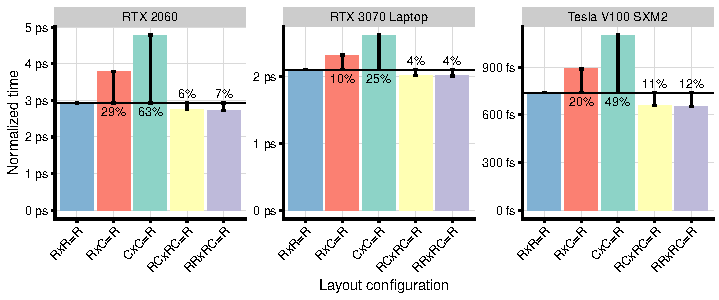
\includegraphics{noarr/plots/matmul_selected.pdf}
    \caption{Speedups of selected layout combinations relative to (row-major) baseline}
    \label{fig:matmul_speedup}
\end{figure}

The result verified that \textbf{RC} is superior to the baseline row-major layout in both input positions. Furthermore, the $R\times C=R$ configuration (often praised on sequential architectures) exhibits worse than the baseline on massively parallel hardware. While this was expected, the primary outcome of this benchmark is methodological: A selection of input and output layouts can be tested systematically without reimplementation effort, while the larger exploration size of the selection (enabled by low coding overhead) provides a solid guarantee that the best-identified solution is indeed a good choice for a high-performance software.


% -----------------------------------------------------------------------------
\subsection{Transformations}\label{sec:transformations}
% -----------------------------------------------------------------------------

The layout-agnostic algorithms can benefit from performance gains achieved by choosing the best layout for a given problem configuration and architecture. However, in real-world scenarios, the layout of the input and output data structures is often prescribed as an inherent part of the algorithm interface or selected by the caller (in the case of generic interfaces).

If the algorithm is complex enough and the performance gap between the prescribed layouts and optimal layouts is high, the data structures may be copied and transformed into their optimally organized counterparts to speed up the algorithm. With \Noarr{}, the transformation can be handled in a generic way. Following our examples with matrices, Listing~\ref{lst:transform} presents the central part of a generic transformer for 2D structures.

\begin{listing}
    \vspace{-10pt}
    \inputmintedcpp{noarr/code-snippets/transform-short.cpp}
    \vspace{-20pt}
    \caption{Key part of transformation routine for 2-index (2D) arrays}
    \label{lst:transform}
\end{listing}

In fact, we are currently extending \Noarr{} to handle the transformations in a generic way for any-dimensional structures, and we are exploring techniques how to select the best way of iterating the structures (e.g., selecting the best ordering of nested loops) in order to optimize memory transfers and caching. However, this research is well beyond the scope of this paper.


\subsubsection{Transformation overhead assessment.}

Employing transformations may be beneficial only under specific circumstances. Simply put, the algorithm must save more execution time than how long it takes to transform all the necessary data. We want to demonstrate the overhead assessment on the previously introduced matrix multiplication example.

We have analyzed the layout transformation overhead for various matrix sizes and layouts. The key results are summarized in Figure~\ref{fig:matmul_comp}. We have observed that in the case of larger matrices ($N>10,000$), the overhead is negligible, primarily because of the asymptotic complexity difference between the transformation algorithm ($\mathcal{O}(N^2)$) and the multiplication ($\mathcal{O}(N^3)$). For smaller matrices (with $N$ around $1000$), the relative ratio of the transformation to computation time expectably increased, and the transformation overhead caused the baseline to perform the best.

\begin{figure}
    \centering
    \includegraphics{noarr/plots/matmul_transform.pdf}
    \caption{Layout transformation times compared to actual matrix multiplication times}
    \label{fig:matmul_comp}
\end{figure}

As demonstrated, deciding whether or when a layout transformation can be beneficial may be complicated; however, with \Noarr{}, both the experiments and the actual decision to apply or not to the transformation can be implemented very quickly.

% Finally, it is worth mentioning that the overhead of the transform algorithm can be reduced by selecting an appropriate copy-ordering for different layouts. The example in Listing~\ref{lst:transform} is designed as optimal for row-major layout, but it may not be optimal for other types of transforms. One of the objectives for the future research is to extract meta-information from the layout structures that would allow us to automatically select the optimal transform strategy (e.g., ordering of the nested for-loops).

% \section{Layout Transformations}\label{sec:transformations}

The layout-agnostic algorithms can benefit from performance gains that are achieved by choosing the best layout for given problem and architecture. However, in real-world scenarios, the layout of the input and output data structures is often prescribed as an inherent part of the algorithm interface, or even selected by the caller (in case of generic interfaces). Here, we show a straightforward way to generate code that transforms the code into the desired layout.


% -----------------------------------------------------------------------------
\subsection{Semi-automated transformation layer}
% -----------------------------------------------------------------------------

An abstract workflow of any data-processing program may be simplified to 3 phases --- \emph{loading} of the data into possible intermediate structures, \emph{execution} of the operation on the data, and \emph{storing} of the contents of possible intermediate structures into the target buffers.

To ensure optimal layout for the execution while keeping the input and output format as prescribed or selected by the caller, an adaptive layer can be introduced between steps 1--2, and 2--3 of the workflow. This layer would handle the transformation of the data from the original `external' input format into the optimal `internal` input format, and from optimal output format to the final output format. Assuming that the memory management in the second step is properly decoupled from array representation, the \emph{layout transformation} in the adaptive layers can be written as a generic routine using \Noarr{} library, as shown on an example for arrays with 2 indexes in Listing~\ref{lst:transform}.

\begin{listing}
    \vspace{-10pt}
    \inputmintedcpp{noarr/code-snippets/transform.cpp}
    \vspace{-20pt}
    \caption{Generic layout transformation routine for 2-index arrays.}
    \label{lst:transform}
\end{listing}

In the example, the transformation function (lines 1--7) operates on two \texttt{bag} structures, copying their contents element by element from a bag with data that use input layout to a bag with the desired layout, effectively performing the layout transformation. A helper function (lines 9--20) further simplifies the data transformation by determining if a layout change is really needed, and executing transformation (and copying the data) conditionally only in that case.

\begin{listing}
    \vspace{-10pt}
    \inputmintedcpp{noarr/code-snippets/matmul_transform.cpp}
    \vspace{-20pt}
    \caption{Outline of layout transformation layer for matrix multiplication example.}
    \label{lst:matmul_transform}
\end{listing}

These transformation routines may be readily used in other algorithms, as demonstrated in Listing~\ref{lst:matmul_transform} that wraps a matrix multiplication algorithm similar to the one from Listing~\ref{lst:matmul}.

We note that it is possible to implement the layout transformation function generically for any layout, for example by adapting the layout objects to work in range-based for-loops. Complex design considerations of the implementation (especially the static forwarding of the dimension identifiers) are however out of scope of the current \Noarr{} implementation.

% -----------------------------------------------------------------------------
\subsection{Exploring all layout combinations}
% -----------------------------------------------------------------------------

Given the possibility to work with arbitrary input and output layouts, we may expand the experiment from Section~\ref{sec:layouts-agnostic} to a larger spectrum of possible combinations of input and output layouts. We utilize the schema from Listing~\ref{lst:matmul_transform} to systematically loop through and benchmark all $6^3$ combinations of the layouts for the tiled matrix multiplication. The results are shown in Figure~\ref{fig:matmul_heatmap_all}.

\begin{figure}
	\centering
	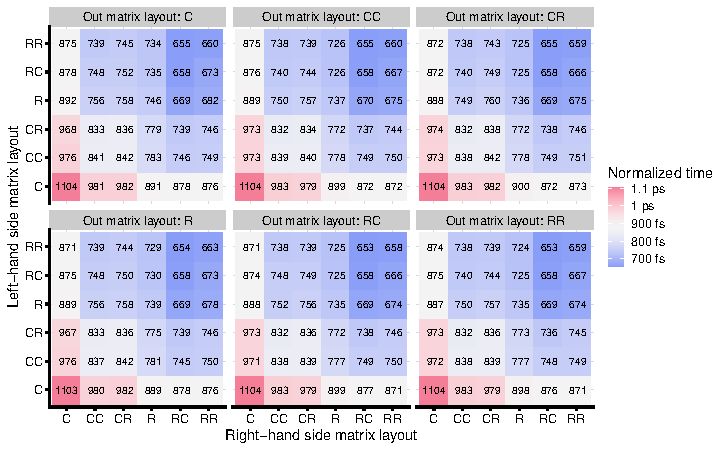
\includegraphics{plots/heatmap_all.pdf}
	\caption{Performance overview of layout combinations in matrix multiplication (X and Y axes represent the layout of right and left operand of the multiplication, layouts of the output are plotted separately). We report the normalized time per asymptotic operation, i.e., wall time divided by $N^3$.}
	\label{fig:matmul_heatmap_all}
\end{figure}

The results imply that the kernel performed best with $\textbf{RR}\times \textbf{RC}=\textbf{RR}$ layout combination, which was expected for tiled algorithm. The layout of input matrices turns out to be very important as the worst configuration ($\textbf{C}\times \textbf{C}$) is almost two times slower than the best one. On the other hand, the performance differences for the output matrix layouts are almost negligible. As in Section~\ref{sec:layouts-agnostic}, the main result is again methodological: The programmers may easily screen through all possible layouts for their data structures, and choose a reliable optimum for inclusion in production software.

% -----------------------------------------------------------------------------
\subsection{Transformation overhead}
% -----------------------------------------------------------------------------

While the algorithm performance is determined mainly by the layout combinations, the absolute performance differences are not huge. For example, the commonly used row-major format (i.e., $\textbf{R}\times \textbf{R} = \textbf{R}$) is only about 12\% slower on selected matrix sizes, which makes it at least competitive. We may therefore ask whether the data transformation overhead would not nullify the benefits of optimal layouts.

% The findings of this semi-automated layout transformation can in reasonably simple programmatic way show insights into the behavior of the specific function in terms of the memory access pattern and caches utilization. With minimal effort, this principle can be applied on multi-stage pipeline algorithms where each stage expects different memory layout for the most optimal computation. 

% However, a duration of the actual transformation needs to be accounted into as well. Depending on the layout pair to be transformed, the size of data and the actionable function, the duration of the transformation can sometimes diminish the performance gain resulted from the optimal layout usage in the selected algorithm. 

To clarify this concern, we have analyzed the layout transformation overhead for various matrix sizes and layouts. The key results are summarized in Figure~\ref{fig:matmul_comp}. We have observed that in the case of larger matrices ($N>10000$), the overhead is negligible, mostly because the asymptotic complexity difference between the transformation algorithm ($\mathcal{O}(N^2)$) and the multiplication ($\mathcal{O}(N^3)$). For smaller matrices (with $N$ around $1000$), the relative ratio of the transformation to computation time expectably increased. (Additionally, smaller matrices benefited more from caches, which make their layout slightly less important.) At that point, the baseline configuration $\textbf{R}\times\textbf{R}=\textbf{R}$ becomes the best option simply because it lacks the transformation overhead.

\begin{figure}
	\centering
	\includegraphics{plots/matmul_transform.pdf}
	\caption{Overhead of the layout transformation compared to actual time spent in the matrix multiplication algorithm. Only selected combinations of the layouts are shown for small and big matrix sizes.}
	\label{fig:matmul_comp}
\end{figure}

Finally, it is worth mentioning that the overhead of the transform algorithm can be reduced by selecting an appropriate copy-ordering for different layouts. The example in Listing~\ref{lst:transform} is designed as optimal for row-major layout, but it may not be optimal for other types of transforms. One of the objectives for the future research is to extract meta-information from the layout structures that would allow us to automatically select the optimal transform strategy (e.g., ordering of the nested for-loops).

\section{Performance Impact of Constant Expressions}\label{sec:perf}

One of the essential features of \Noarr{} is that the first-class structures propagate along with their templated types, allowing us to embed statically defined properties (most importantly, the constant dimensions of the structure) into the type itself. Therefore, the compiler can employ optimizations like compile-time evaluation of constant expressions or exact-sized loop unrolling, which might lead to more efficient execution or even automated vectorization. These optimizations rarely produce a game-changing improvement in performance; thus, the programmers often overlook them. However, utilization of \Noarr{} structure will introduce them naturally so the result code could run faster without any additional effort whilst maintaining other benefits like memory allocation decoupling or coding in a layout-agnostic manner.

To present the main idea, let us have an array $A$ of $N$ vectors in $\mathbb{R}^D$ where $N$ is a variable, and $D$ is a constant\footnote{If the code needs to handle several different dimensionalities $D$, it will be compiled for each $D$ independently thanks to the power of C++ templates.}. We want to compute the Euclidean distance between every vector in the array and given vector $q$ (e.g., to find $k$ nearest vectors, which is quite a typical task in many data-processing problems):

\begin{minted}[fontsize=\scriptsize]{c++}
  for (size_t i = 0; i < N; ++i) {
    float dist = 0.0f;
    for (size_t d = 0; d < D; ++d) {
      float diff = A[i*D + d] - q[d];
      dist += diff * diff;
    }
    dist = std::sqrtf(dist); // ...
  }
\end{minted}

When $D$ is a constant, the compiler could unroll the loop entirely without additional branches. It might even attempt to unroll the outer loop if $D$ is sufficiently small. The speedup achieved by having constant $D$ may easily reach factor $3\times$ for very small values of $D$ (e.g., $D=2$)\footnote{If we measure only the Euclidean distance computation.}.


% -----------------------------------------------------------------------------
\subsection{Indexing performance}
% -----------------------------------------------------------------------------

To demonstrate the impact of \Noarr{} structures, we have selected a 3D stencil problem as an example. Stencil is a simple function computed iteratively for every element of a regular grid. We have used an averaging stencil executed on a 3D grid which could be used as an approximative simulation of gas diffusion, for instance. Our objective is to emphasize the difference between situations when the grid dimensions are constant (at compile time) and when they are determined at runtime.

The main code of the stencil is in Listing~\ref{lst:stencil_base}. Run-time variables \texttt{size\_x}, \texttt{size\_y}, and \texttt{size\_z} denote the dimensions of the cube. The first part of this experiment aims at exposing only the compile-time optimizations of index computations, so we ensure that no optimizations related to constant dimensions are performed. Please note that the loops do not visit points residing on the faces of the grid so that we can ignore the border cases of the stencil function; thus, there are no branches in the code which leads to simpler and more stable measurement. 

\begin{listing}[h]
    \vspace{-10pt}
    \inputmintedcpp{noarr/code-snippets/stencil_base.cpp}
    \vspace{-20pt}
    \caption{Main stencil for-loop}
    \label{lst:stencil_base}
\end{listing}

A na\"{i}ve C-like implementation of the internal \texttt{stencil} function is presented in Listing \ref{lst:stencil_trivial}. It uses the same variables in the loop to index the data pointers, preventing the compiler from doing more elaborate compile-time optimizations. This code is used as a baseline for the performance comparison.

\begin{listing}[h]
    \vspace{-10pt}
    \inputmintedcpp{noarr/code-snippets/stencil_trivial.cpp}
    \vspace{-20pt}
    \caption{Na\"{i}ve implementation of stencil function}
    \label{lst:stencil_trivial}
\end{listing}
\vspace{-10pt}

Making the dimensions constant may help the compiler to generate more optimal code. In C++, this can be achieved simply by defining the \texttt{size\_*} variables as \texttt{constexpr}; however, such constants need to be declared at the global level, which significantly undermines any encapsulation or reusability of the code. Better way is to use fix-sized containers like \texttt{std::array} and make the stencil code templated so it can be used with any compatible containers (including \texttt{std::vector}).

\begin{listing}[h]
  \vspace{-10pt}
  \inputmintedcpp{noarr/code-snippets/stencil_noarr.cpp}
  \vspace{-20pt}
  \caption{\Noarr{} implementation of stencil with constant-sized \texttt{array}}
  \label{lst:stencil_noarr}
\end{listing}
\vspace{-10pt}

\Noarr{} provides a fixed layout structure \texttt{array}, which fulfills a similar role, but it can be easily integrated into more complex nested structures (even with custom layouts). Listing \ref{lst:stencil_noarr} presents the internal \texttt{stencil} rewritten for \Noarr{}. The dimensions of the grid are no longer passed as variables, but they are embedded in the type of the \texttt{bag} structure as constants. Line $1$ shows the assembling of the layout structure using a predefined \texttt{array} template.

To evaluate the performance, we have selected a grid of a specific size ($2^{20} \times 32 \times 32$) which confines the meaning of the diffuse simulation for a specific environment (e.g., gas in a pipe). The main reason is that the performance improvement caused by the compile-time optimizations is difficult to measure on regular structures since it takes only a small portion of overall time (especially when the computation causes many cache misses). This shape requires more index computations relative to other operations, making the difference more pronounced in the measurements.

\begin{figure}[h]
  \vspace{-10pt}
	\centering
	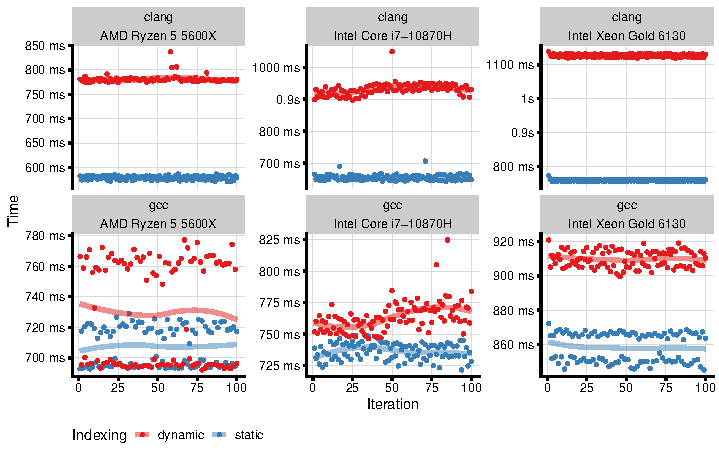
\includegraphics{noarr/plots/stencil.pdf}
	\caption{Wall times of $100$ stencil iterations (plotted lines represent the local regression of the measured times)}
	\label{fig:stencil}
  \vspace{-10pt}
\end{figure}

Figure \ref{fig:stencil} shows the comparison results of the two presented stencil implementations on three platforms using two compilers. The benefits of compile-time optimizations are visible on every platform and with both tested compilers, albeit there is only a small difference in some configurations. The details regarding the experimental methodology are summarized in Appendix~\ref{appendix:methodology}.


% -----------------------------------------------------------------------------
\subsection{Constant-loops optimizations}
% -----------------------------------------------------------------------------

The second part of this experiment extends the compile-time optimizations to the nested stencil grid loops. It requires replacing \texttt{size\_*} variables in the main loops (Listing \ref{lst:stencil_base}) with constants (i.e., \texttt{constexpr} or template arguments) so the compiler has enough information to perform exact loop-unrolling and better vectorization-related optimizations.

\begin{listing}[h]
  \vspace{-10pt}
  \inputmintedcpp{noarr/code-snippets/stencil_base_bag.cpp}
  \vspace{-20pt}
  \caption{Updated stencil for-loop with \texttt{bag} structure}
  \label{lst:stencil_base_bag}
\end{listing}
\vspace{-10pt}

However, converting these variables to constants may be quite tedious, especially if we want the code to be generic for both constant and non-constant scenarios. This particular issue can be easily overcome by utilization of \Noarr{} \texttt{bag} structures. Having the layout information encoded both in the structure type and the object, method \texttt{get\_length} can query dimension sizes and returns a constant or variable based on the layout specification, all this being decided at compile time. The grid loop function from Listing \ref{lst:stencil_base} needs to be rewritten as demonstrated in Listing~\ref{lst:stencil_base_bag}.

\begin{figure}[H]
  \vspace{-10pt}
	\centering
	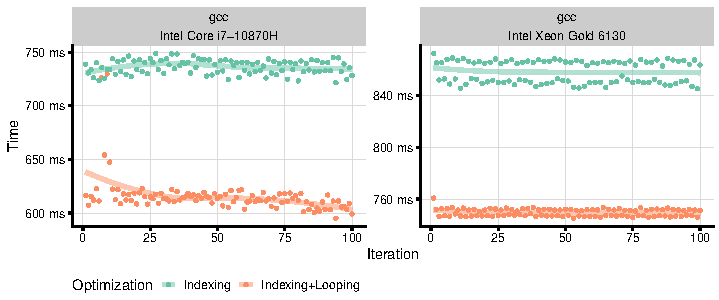
\includegraphics{noarr/plots/stencil_loop.pdf}
	\caption{Stencil execution times of two optimizations --- compile-time \emph{indexing} and the addition of constant-induced loop unrolling (\emph{indexing+looping})}
	\label{fig:stencil_wloop}
  \vspace{-10pt}
\end{figure}

Figure \ref{fig:stencil_wloop} presents the performance improvements of exposing constant variables to the grid iteration loop. We have included only measurements of programs compiled by \texttt{gcc} since \texttt{clang} was not able to take advantage of the constant values when they are passed through the \texttt{bag} structure interface.

\section{Implementation and Technical Insights}\label{sec:implementation}

The \Noarr{} library\footnote{\url{https://github.com/ParaCoToUl/noarr-structures}} is logically divided into three levels, each building on top of the previous one: \emph{structures}, \emph{functions}, and \emph{object wrappers}. The first two layers provide a rather low-level functional approach, while the last one encapsulates the first two into a more traditional C++ object-oriented design.

% -----------------------------------------------------------------------------
\subsection{Structures} 
% -----------------------------------------------------------------------------

A \emph{structure} is an object that stores information about a data layout. It exposes the information via a~simple interface, providing its size in bytes (\texttt{size()}), the range of indices it supports (\texttt{length()}) and a current offset from the beginning of the structure in bytes (\texttt{offset()}).

The most trivial structure is \texttt{scalar} (Listing \ref{lst:scalar}), which wraps the `base' values to be used in more complex layouts. Scalar often wraps simple types like \texttt{float}, but it can also wrap any fixed-size C++ type (such as \texttt{struct} or \texttt{std::tuple}). The methods \texttt{length()} and \texttt{offset()} of \texttt{scalar} always return $0$ because \texttt{scalar} represents only a single element.

\begin{listing}[h]
  \vspace{-10pt}
  \inputmintedcpp{noarr/code-snippets/scalar.cpp}
  \vspace{-20pt}
  \caption{A core part of the \texttt{scalar} structure used for wrapping simple values}
  \label{lst:scalar}
\end{listing}

The \texttt{array} structure (Listing \ref{lst:array}) is more complicated: Like \texttt{std::array}, it represents a~fixed-size array with a named dimension and statically defined number of elements of a given \emph{substructure}~type. Unlike \texttt{scalar} which wraps a \emph{trivial type}, \texttt{array} is contains a \Noarr{} \emph{structural type}.

An important aspect of the structures is their ability to be combined and nested to create a \emph{structure tree}. For instance, the composition of \texttt{scalar} and \texttt{array} is quite straightforward:
\begin{itemize}
\item\mintinline[fontsize=\scriptsize]{c++}{array<'a', 10, scalar<float>>}
defines an array of $10$ \texttt{float}s,
\item\mintinline[fontsize=\scriptsize]{c++}{array<'i', 4, array<'j', 8, scalar<int>>>}
represents a~$4\times8$ row-major integer matrix layout,
\item\sloppy\mintinline[fontsize=\scriptsize]{c++}{array<'j', 8, array<'i', 4, scalar<int>>>}
represents the same matrix in a column-major layout.
\end{itemize}

\begin{listing}[h]
  \vspace{-10pt}
  \inputmintedcpp{noarr/code-snippets/array.cpp}
  \vspace{-20pt}
  \caption{\Noarr{} \texttt{array} structure (some methods are omitted for brevity)}
  \label{lst:array}
\end{listing}

All structures inherit from class \texttt{contain}, which has several purposes: It serves as recursive storage for the wrapped structure, holds some useful meta-information about the nested substructures, and stores possible additional data for the structure, such as dynamic dimension length or the current offset index. Querying for various properties, which is its main purpose, is demonstrated in Listing \ref{lst:array}. The \texttt{array} implements the \texttt{size()} function using the information (size) from its immediate substructure (line $4$). In the example, queries work recursively on subsequent immediate substructures until the recursion is halted in \texttt{scalar::size()}. Using this mechanism, \texttt{contain} allows us to create the nested hierarchy of the structure tree easily.

There are several other built-in structures in \Noarr{} library, such as \texttt{vector} and \texttt{tuple} (analogical to \texttt{std::vector} and \texttt{std::tuple}), which provide sufficient arsenal for composing memory layouts of many regular-shaped data structures. Moreover, the library design makes it open for extensions, and programmers may implement additional custom layout structures.


% -----------------------------------------------------------------------------
\subsection{Functions}
% -----------------------------------------------------------------------------

\Noarr{} \emph{functions} are C++ \mintinline{c++}{constexpr} functions that serve as an expressive tool for obtaining complex information from the structure trees. They are used to compute offsets for memory pointers to provide indexation, transform structures, and query dimension lengths using a single, extensible functional interface.

Calling function \texttt{f} on a structure \texttt{s} is achieved using the (overloaded) `pipe' operator \texttt{|}. Expression \texttt{s | f} denotes that \texttt{f} is applied on \texttt{s} (note this may sometimes differ from \texttt{f(s)} as detailed later in this section).

For example, the function \texttt{get\_length()} traverses structure tree and calls \texttt{length()} on a substructure with the given dimension name:
\begin{minted}[fontsize=\scriptsize]{c++}
  size_t i_len = a_structure | get_lenght<'i'>();
\end{minted}

The function \texttt{set\_length()} proceeds similarly, but when a matching substructure is found, the whole structure is reconstructed to carry the new length. The following example shows that functions can be additionally chained one after another. Notably, all structures are immutable, which allowed us to ensure that \texttt{unsized\_s} does not carry any unnecessary data:
\begin{minted}[fontsize=\scriptsize]{c++}
  auto unsized_s = vector<'i', vector<'j', scalar<float>>>();
  auto sized_s = unsized_s | set_length<'i'>(4) | set_length<'j'>(8);
\end{minted}

A function application on a structure may fail, such as when querying a~length of a non-existing dimension. We say the function is \emph{not applicable} on a~structure. Taking the aforementioned two functions into account and the fact that every structure forms a structure tree, it is possible that a~function is not \emph{directly applicable} on the topmost structure but is applicable on some structures in the structure tree. For this reason, we distinguish three \emph{piping mechanisms} that govern different means of the function-structure application:

\begin{itemize}
    \item \emph{Top application} (or \emph{direct application}). This is the simplest form of piping, where \texttt{s | f} is equivalent to \texttt{f(s)}. In other words, the function is applied directly to the topmost structure. 
    \item \emph{Get application}. Given the piping \texttt{s | f}, if \texttt{f(s)} is not applicable the piping mechanism attempts to apply \texttt{f} to the substructures of \texttt{s} recursively. It fails if \texttt{f} does not apply to any of the substructures or if it applies to more substructures. The trivial representative being \texttt{get\_length()}, because there should be exactly one node in a structure tree with a specified dimension.   
    \item \emph{Transform application}. \texttt{s | f} either results in top application when \texttt{f(s)} is applicable or \texttt{f} is transformatively applied on all \emph{direct} substructures of \texttt{s}. If the latter, the structure is reconstructed with these changes to the substructures. 
\end{itemize}

The piping mechanism is implemented using C++ \mintinline{c++}{constexpr} functions and metaprogramming. Together with the static nature of substructure hierarchies that encompasses the structure layer, the implementation is very efficient since it provides the necessary space for compiler optimizations. We can demonstrate this by precisely describing the operations executed when a function with the get application is applied to a structure. Let us have the following structure and function:
\begin{minted}[fontsize=\scriptsize]{c++}
  auto v4 = vector<'a', vector<'b', vector<'c', vector<'d', scalar<int>>>>>();
  auto f = get_length<'d'>();
\end{minted}
Expression \texttt{v4 | f} must perform a traversal of the structure tree to find the matching dimension. Fortunately, the way the structures and functions are implemented ensures that there is no run-time loop in the implementation. Because all substructures are known in compile-time, the traversal loop is unrolled using metaprogramming techniques. Furthermore, because the values are also known at compile-time, the result can be partially evaluated and, in turn, \emph{no run-time code is generated}. In summary, applying \texttt{v4 | f} produces four unrolled function applications, three of which produce no operation at all (and usually get discarded by a compiler), and only one results in calling \texttt{length()} on a~substructure that can be evaluated by the compiler.


% -----------------------------------------------------------------------------
\subsection{Object wrappers} 
% -----------------------------------------------------------------------------

Object wrappers provide object-oriented management of structures, functions, and the actual data. \Noarr{} library offers two kinds of such objects --- structure \emph{wrappers} and \texttt{bags}.

A \texttt{wrapper} simplifies the work with structures by bundling the applications of the most common \Noarr{} functions into member methods. That way, with a wrapper \texttt{w} of a structure \texttt{s} we can directly write \mintinline{c++}{w.get_length<'d'>()} instead of \mintinline{c++}{s | get_length<'d'>()}.

A \texttt{bag} provides the same interface as a~\texttt{wrapper} but also contains a pointer to the underlying memory. To work with the data, it implements a~member method \mintinline{c++}{at<Dims...>(idxs...)} that is used to index the data pointer with respect to the enveloping structure layout. This method is a wrapper for the library function \texttt{get\_at}. Without using a \texttt{bag}, the indexing might look like this:
\begin{minted}[fontsize=\scriptsize]{c++}
  auto s = array<'j', 8, array<'i', 4, scalar<float>>>();
  float* ptr = allocate_memory_bytes(s.size());
  float x = s | get_at<'i', 'j'>(ptr, 2, 3);
\end{minted}
The \texttt{bag} binds the layout together with data, systematizing the computation on the last line as follows:
\begin{minted}[fontsize=\scriptsize]{c++}
  auto b = bag(s, ptr);
  float x = b.at<'i', 'j'>(2, 3);
\end{minted}

Furthermore, to manage an explicitly bound external pointer, \texttt{bag} can also allocate the underlying memory automatically if no pointer is given (i.e., it also carries the semantics of a smart pointer). Technically, \texttt{bag} can belong to either one of two semantic groups according to the way it acquires data:
\begin{itemize}
    \item \emph{Owning semantics.} The bag is constructed only with a structure to envelop. The data pointer of exact length is automatically allocated using standard memory management (e.g., by \texttt{unique\_ptr}), and the length is determined by calling \texttt{size()} on the wrapped structure.
    \item \emph{Borrowing semantics.} The bag is constructed with both structure and data pointer. In this case, the deallocation, as well as ensuring the proper data-block length, has to be enforced by the caller.
\end{itemize}



% \begin{enumerate}
%     \item \emph{Structures} --- .
%     \item \emph{Functions} --- C++ pure constexpr functions that serve as an expressive tool to obtain complex information from a tree of structures.
%     \item \emph{Object wrappers} --- Classes that provide object oriented wrappers on top of the previous layers.
% \end{enumerate}

% \Noarr{} library distinguishes three objects:
% \begin{itemize}
%     \item \texttt{Structure} A small, tree-like object, that represents the structure of the data. It does not contain the data itself, nor a pointer to the data. It can be thought of as a function that maps indices to memory offsets (in bytes). It stores information, such as data dimensions and tuple types.
%     \item \texttt{Data} A continuous block of bytes that contains the actual data. Its structure is defined by a corresponding Structure object.
%     \item \texttt{Bag} Wrapper object, which combines structure and data together.
% \end{itemize}

% \subsection{Structure}

% Supported layouts:
% \begin{itemize}
%     \item \texttt{Containers} Vector or array. 
%     \item \texttt{Scalars} int, float, size\_t.
%     \item \texttt{Tuples} Ordered set of previous two.
% \end{itemize}

% \subsection{Functions}

% Means of modifying structures and applying them on data.

% \begin{itemize}
%     \item \texttt{get\_length get\_offset} ... read
%     \item \texttt{set\_length, fix} ... modify  
%     \item \texttt{get\_at} ... index
% \end{itemize}

% \subsection{Internal representation}

% Thx to majority of logic is in functions, actual layout structure is very simple.

% implemented as a tree of sub structures ... easily extensible ... show simple example (reverse vector)

% \subsection{Data and Bag}

% Data must be continuous (no jagged).

% Bag acquires data 2 ways:
% \begin{itemize}
%     \item \emph{borrowing semantics} gets data via pointer as constructor param
%     \item \emph{owning semantics} allocates data using standard memory management
% \end{itemize}



% nasledujici text je zkopirovan z paper.tex (brainstorming), bure potreba to jeste poradne rozmyslet (aby tahle sekce nebyla moc tlusta, ale byla vystizna); rozhodne to nema byt reference kodu
% (quick peek on the most important structures + how they are implemented, this must not look like a reference)

% 1. built-in struktury vector, array, scalar, tuple
% 2. ako sa s nimi pracuje: bag, set\_length, indexovanie, structure wrapper
% 3. impl. details?

% \section{Flexible data layout}

% 1. noarr je plne rozsiritelny na definovanie vlastneho layoutu. ukazat na jednoduchom priklade
% ako sa to robi (reverse-vector/matrix napr.)
% 1.1. vysvetlit noarr::compose <=> std::tuple
% 1.2. vysvetlit vyznam preco vsetko je constexpr  
% 2. na vacsom priklade ukazat predosle body (cache aware layout na matmul v CUDE) + porovnat s trivial impl

% \section{Easy switch between layouts in noarr workflows}

% 1. ukazat, ze noarr sturktury su vo funkcii/kerneli zamenne
% 2. ukazat moznost jednoduchej transformacie medzi layoutmi
% 2.1. ukazat funckie na vlozenie transformacnej vrstvy do algoritmu
% 3. na vacsom priklade ukazat predosle body - full-blown aplikacia transformacnych vrstiev + layoutingu (porovnat wall time [i s transformaciou] oproti algoritmu s trivialnym layoutom)

\section{Related Work}\label{sec:relwork}

A significant group of works that touch the problem of memory layouts are parallel programming languages such as X10~\cite{charles2005x10}, Chapel~\cite{chamberlain2007parallel} or Legion~\cite{bauer2012legion}. Apart from providing syntax for simple parallel code expression, these languages allow for data decomposition into regions that can be mapped within the same memory space or more complex non-uniform memory spaces. Hence, the memory layout expression addressed by these works is only researched to the point of high-level data distribution among processing elements.

Application-specific library generators, or \emph{active libraries}, also utilize memory layouts. The most known representatives are ATLAS~\cite{whaley1998automatically}, SPIRAL~\cite{puschel2004spiral} and FFTW~\cite{frigo1998fftw} specializing in linear algebra, signal processing, and Fast Fourier Transform, respectively. They are trying to mitigate portability issues of manually optimized programs by selecting the best interprocedural optimizations for the hosting system using autotuning. Usually, these optimization strategies include some form of memory layout selection. It is important to note that active libraries target different stages in programming than \Noarr{}; rather than performing the layout selection from the hardcoded set of layouts, \Noarr{} provides means to \emph{implement} such layout selections in a more extensible and object-oriented way.

The most related works we found are Kokkos \cite{9485033}, and GridTools \cite{AFANASYEV2021100707}. These libraries allow the coupling of arbitrary data structures with memory layouts which can be either selected from a set of predefined layouts or programmatically customized.

GridTools specialize in block-structured grid applications such as combustion, seismic, and weather simulations, working with generalized stencil-like patterns. The library defines a storage infrastructure component that controls the layout, alignment, and padding of stored data fields. A layout is specified in code at compile time by selecting one of the predefined target backends, each well suited for a specific use case, such as vector instructions or GPU kernels. The library can be extended with new programmer-specified backends, but the layout can be altered only by permuting dimension order in a regular $n$-dimensional array. 

An interesting approach is taken in the Kokkos library, which specifies the \texttt{View} class that couples the definition of data memory space, allocation, and layout altogether using C++ policy classes, yielding an object of similar functionality as our \texttt{bag}. The memory resource and allocation mechanism are abstracted and defined by the template argument. Kokkos provides multiple memory spaces such as \texttt{HostSpace}, \texttt{CudaSpace}, \texttt{CudaHostPinnedSpace}, thus representing CPU and GPU physical memory and their combinations.

In Kokkos, the memory layout is either implicitly deduced from the memory space or explicitly specified as another template parameter. The library implements row and column-major layouts together with the layout with strides with custom sizes. Kokkos allows user-defined memory layouts by defining a new layout policy and implementing a function that defines a bijective mapping between index space and memory addresses. However, this mapping must be defined on a regular $n$-dimensional array, using a minimal API that fits the \texttt{View} class.

Language-wise, our approach is similar to (and inspired by) known concepts from functional programming. Materialized, first-class composable references to sub-structures uncoupled from data have been extensively studied as optics~\cite{foster2007combinators}. In particular, the internal structures that implement the selection of array slices at certain indexes are similar to the concept of indexed lenses --- kind of references that transparently provide information about the current index in a complicated structure, as summarized by Clarke et~al.~\cite{clarke2020profunctor} In the future, it might be interesting to examine whether more advanced optics may be modeled in C++ for array accesses, e.g., expressing repeated data accesses similarly to lens-based traversals or reconstructing the user-facing indexes from known offsets using isomorphisms.


% TiDa and GridTools specialize in block-structured grid applications such as combustion, seismic, and weather simulations, working with generalized stencil-like patterns. TiDa allows the programmer to express data locality and layout at the array construction by declaring how the data is divided into regions to be accessed by different processing elements (such as NUMA nodes), which are further divided into tiles for finer layout granularity.


% Extensive research has been performed in choosing optimal layouts concerning a provided algorithm. For example, Sharma et al.~\cite{10.1145/2747875} investigated a transformation technique called array interleaving, which combines the storage of data elements from multiple arrays to achieve better data locality. Sung et al.~\cite{sung2010data} presented compiler optimization that enables data layout transformation for structured grid codes with dynamically allocated arrays (e.g., stencil functions). These involve source-to-source program transformation to generate functions that can transform the data into a `better' layout with more locality. Both authors observed performance increases, reductions in memory transfers, and improvements in memory access patterns.


% parallel libraries with much wider functionalities than just layout transformations:
% \begin{enumerate}
%     \item \emph{kokkos} \cite{9485033,CARTEREDWARDS20143202}
%     \subitem provides class View that defines memory space, allocation, layout alltogether via policy classes.
%     \subitem Memory space template represents allocation mechanism. Kokkos imlpements multiple types: HostSpace, CudaSpace, CudaHostPinnedSpace indexing is implemented by DeviceType, a policy class.
%     \subitem Layout is statically inlined, primarily LayoutLeft, LaoutRight, LayoutStride.
%     \subitem on top of that, there is third policy class. Memory Traits. Provides additional info about memory behavior --- whether to utilize texture memory in CUDA, atomic access, ...
%     \subitem View in its constructor defines sizes of dimensions, but can be provided staticaly via template argument as well. In its constructor, it allocates data according to memory space policy. It can be coppied to create a view of the data. effectively creating shared-ptr semantics over the data.
%     \item \emph{TiDa} \cite{tida}. library supports programs operating on block-structured grid applications such as combustion, seismic, weather simulations and image processing. Divides data into regions to improve data locality on NUMA nodes. regions are divided into tiles improve cache reuse.
%     \item \emph{GridTools} \cite{AFANASYEV2021100707}. Only custom possibility is to permute dimensions in ndarray. Other than that, it supports general layouts for some common cases (vectorization, gpu).
% \end{enumerate}

% works targeted on finding optimal memory layout and layout transformation:
% \begin{enumerate}
%     \item \cite{10.1145/2747875} efficient layout transformation via array interleaving to improve memory accesses for SIMD FUs, SMPs, vector registers. Achieves decrease in memory energy consumption 6-36 percent.
%     \item \cite{sung2010data} presents compiler optimization that enables data layout transformation for structured grid
%     codes (stencil, fluid dynamics, heat dicipation) in CUDA. It involves source to source compilation that generates transformative functions that result in layout with better data locality. The code must be further compiled by NVCC (or other suitable) compiler.   
% \end{enumerate}

% purely functional haskel libarary for writing multi-dimensional arrays.


% -----------------------------------------------------------------------------
\section{Conclusion}\label{sec:conclusion}
% -----------------------------------------------------------------------------

We have presented a new high-performance approach for managing the complexity of offset computation in array-like data structures in modern C++. We introduced first-class layout structures that can be used to describe complex array layouts and run the required offset computations. The implementation is based on C++ template metaprogramming, exposing a rich interface for manipulating the structures with index mnemonics while enabling many compiler optimizations by properly separating static compile-time parameters and known constants from dynamic data.

The technique promotes complete decoupling of array indexing from memory allocation, which makes it applicable for many scenarios, including direct processing of memory-mapped files or re-using the same data structure layout in various memory spaces (e.g., offloading computations to GPUs). We showed that the layout structures, combined with the C++ templating system, make it easier to create layout-agnostic algorithms and functions, leading to a simpler selection of optimal layouts for a given hardware platform and problem configuration. Additionally, the utilization of layout structures makes it easier to create semi-automated layout transform routines, which can improve the performance of many algorithms.

We have implemented the proposed ideas in \Noarr{}, a prototype library demonstrating the viability of the approach. We demonstrated the benefits in several examples and experiments; most importantly, we showcased the ability to write shorter program source code that promotes easier experimentation and compilation into faster solutions. The library is publicly available as an open-source portable to all mainstream compilers, including CUDA \texttt{nvcc}, and may be readily used in designing new libraries that consider performance a priority. We expect that the approach will simplify the research focusing on optimizations and automatic tuning of the performance of complex parallel algorithms.

% \subsection*{Acknowledgements}

% This work was supported by Charles University institutional funding SVV 260451.

% \appendix

\section{Experimental Methodology}\label{appendix:methodology}

The main objective of the benchmarking was to measure the speedups achieved by different layout combinations to support the claims mentioned in the work\footnote{More details and the data are in the replication package \url{https://github.com/asmelko/ica3pp22-artifact}.}. A more complex performance evaluation is beyond the scope of this paper and is planned in future work.

% -----------------------------------------------------------------------------
\subsection{GPU benchmarking setup}
% -----------------------------------------------------------------------------

In the results, we present mainly the kernel execution times measured by the high-precision system clock, which is available on all platforms. The relative standard deviations in $20$ collected measurements of each result were less than $5$\% of the mean value in all cases, so we report only the mean values.

Due to the page limit, the presented results were limited to matrices of sizes $(1008\times 1008)$ and $(10,080\times 10,080)$. However, more extensive testing on other problem instances, including a broader range of matrix sizes and non-square matrices, exhibited similar results.

The results were collected on the following platforms:
\begin{itemize}
    \item NVIDIA Tesla V100~SXM2 (Volta, CC 7.0, $1.3$GHz), Rocky Linux 8
    \item NVIDIA GeForce RTX 2060 (Turing, CC 7.6, $1.7$GHz), Windows 10
    \item NVIDIA GeForce RTX 3070 laptop (Ampere, CC 8.6, $1.6$GHz), Windows 11
\end{itemize}

All platforms used CUDA toolkit 11.6 with an up-to-date driver. These devices represent three of the most recent Nvidia architectures and three typical hardware platforms (server, desktop PC, and laptop). Hence, we claim that the measurements sufficiently represent contemporary CUDA-enabled GPUs.


% -----------------------------------------------------------------------------
\subsection{CPU benchmarking setup}
% -----------------------------------------------------------------------------

We ran the kernel in $100$ iterations for the stencil benchmark, plotted the local regression outlining the mean value, and distinguished the outliers.
The measurements were conducted using the following CPUs:
\begin{itemize}
    \item AMD Ryzen 5 5600X (hi-end desktop CPU, $3.70$GHz), Windows 10
    \item Intel Core i7-10870H (laptop CPU, $2.20$GHz), Windows 11
    \item Intel Xeon Gold 5218 (server CPU, $2.3$GHz), Rocky Linux 8.
\end{itemize}

Due to the fact that some compilers may optimize \texttt{constexpr} expressions better than others, we compiled the benchmark using \texttt{clang++} v$12$ and \texttt{g++} v$11$ compilers with \texttt{-03} flag.
We also compiled the stencil benchmark using the MSVC C++ compiler, but the results showed that it could not sufficiently optimize \Noarr{} code in the current version; hence, MSVC results are not included.

All benchmarking datasets were synthetic, with data sampled randomly from the same uniform distribution. We consider synthetic validation sufficient since the performance of the benchmarked algorithms is not data-dependent.



% \documentclass[preprint,12pt]{elsarticle}
% \usepackage{amssymb}
% \usepackage{amsfonts}
% \usepackage[utf8]{inputenc}
% \usepackage{graphicx}
% \usepackage{subcaption}
% \usepackage{xcolor}
% \usepackage{color}
% \usepackage{url}
% \usepackage{booktabs}

\definecolor{bluekeywords}{rgb}{0,0,1}
\definecolor{classgreen}{rgb}{0.17,0.57,0.68}
\definecolor{greencomments}{rgb}{0,0.5,0}
\definecolor{redstrings}{rgb}{0.64,0.08,0.08}
\definecolor{black}{rgb}{0,0,0}
\definecolor{blueattributes}{rgb}{0.37,0.52,0.62}
\definecolor{interfaceyellow}{rgb}{0.60,0.66,0.11}
\definecolor{directivepink}{rgb}{0.9,0.6,0.95}

\graphicspath{ {./crosscorr/src/img/} }


\chapter{Efficient GPU-accelerated Parallel Cross-correlation}

% \author{Karel Maděra}
% \ead{karelmad@email.cz}

% \author{Adam Šmelko}
% \ead{smelko@d3s.mff.cuni.cz}

% \author{Martin Kruliš}
% \ead{krulis@d3s.mff.cuni.cz}

% \affiliation{organization={Department of Distributed and Dependable Systems, Charles University},
%             city={Prague},
%             country={Czech Republic}}

% \begin{abstract}
% Cross-correlation is a data analysis method widely employed in various signal processing and similarity-search applications. Our objective is to design a~highly optimized GPU-accelerated implementation that would speed up the applications and also improve energy efficiency since GPUs could be more efficient than regular CPUs. There are two rudimentary ways to compute cross-correlation --- a definition-based algorithm that tries all possible overlaps and an algorithm based on the Fourier transform, which is much more complex but has better asymptotical time complexity. We have focused mainly on the definition-based approach which is better suited for smaller input data and we have implemented multiple CUDA-enabled algorithms with multiple optimization options. The algorithms were evaluated on various scenarios, including the most typical types of multi-signal correlations, and we provide empirically verified optimal solutions for each of the studied scenarios.
% \end{abstract}


% \begin{keyword}
%     cross-correlation \sep GPU \sep CUDA \sep parallel \sep algorithm \sep caching \sep optimizations
% \end{keyword}

% \end{frontmatter}

%% \linenumbers

%% main text

\section{Introduction}

Signal processing and analysis are essential in a plethora of applications ranging from video analysis, image matching, audio pattern recognition, or processing sensory inputs in various domains in physics, biology, pharmacy, or medicine~\cite{Kapinchev2015}. Cross-correlation is one of the basic methods employed in signal processing since it provides a metric that compares two signals and allows us to detect the best overlap including the relative shift between two signals.

In this work, we focus solely on the efficiency of the cross-correlation algorithm implementation and we aim to design optimizations that should speed up the computation. We tackle the problem with parallel computing, namely employing contemporary GPU accelerators which are particularly suited for data-parallel tasks. Although the task seems simple at first glance, achieving optimal efficiency is quite challenging due to the unique lock-step execution model of the GPUs which is placed in contrast with the workload imbalance that arises from a straightforward parallel implementation of cross-correlation. Furthermore, the GPUs often suffer from data-throughput issues which are raised by the fact the GPU memory needs to feed tens of thousands of computing cores; hence, we need to design an algorithm that promotes sharing loaded inputs among the cores by cleverly caching data in shared memory or registers. Having a highly optimized, GPU-accelerated implementation of cross-correlation can be beneficial for many applications, especially when the inputs are large or when they need to be processed in real-time. Furthermore, the GPU can achieve a better watt-to-performance ratio than the CPU when used efficiently, so our effort can contribute to power consumption savings in the long run.

Each application of cross-correlation has slightly different parameters, depending on the size of the correlated signals or the number of instances being computed simultaneously. For instance, computing one instance of cross-correlation of two large signals would use a different optimization algorithm than computing a correlation between one small signal and a long sequence of medium-sized signals (i.e., searching for a pattern in a video sequence). Thus, our second aim is to compare and analyze the most typical applications of cross-correlation and find the best algorithm for each type.

There are basically two approaches to computing a cross-correlation. A~na\"{i}ve (or definition-based) implementation that directly follows the mathematical definition (with time complexity of ${\cal O}(N^2)$, where $N$ is the size of both input signals) and an implementation that uses a Fourier Transform (FT) which has better asymptotical complexity (${\cal O}(N \log N)$), but also higher computational overhead. We are focusing solely on the definition-based implementations where the actual code optimizations can be explored and which is more suitable for computing multiple instances of smaller signals. The FT-based algorithm can be implemented using highly optimized libraries like cuFFT, which is currently not interesting from the perspective of basic research in parallel computing and optimizations. However, we have implemented a cuFFT version of cross-correlation as well so we can compare and evaluate both approaches empirically.


\subsection{Motivational application}\label{sec:intro-motivation}

Our research was motivated by material analysis --- detecting material defects by electron microscope. The method uses the microscope to scan the surface of a material in a raster pattern. It projects an electron beam towards individual points in the raster and collects a \emph{backscatter diffraction pattern} for each point. In computer science terms, the method collects a grey-scale image for each point in an input grid. For the selected material, there is a reference diffraction pattern that would be expected for a material without any defects. The collected images are compared with the reference image to detect possible distortions (e.g., translations, rotations, or warps) and these distortions can be interpreted as defects.

The comparison of measured and expected diffraction patterns is performed by dividing the images into multiple corresponding areas (i.e., areas with the same sizes and coordinates in both images) and cross-correlation is used to determine a relative shift of these two areas in the images. Thus we need to compute a cross-correlation of $N$ samples from one signal with $N$ samples from $M$ signals. The $N\cdot M$ easily reaches an order of millions, but the size of the areas is relatively small. Therefore, there is a lot of potential for parallelization, but it also means that the FT-based approach is likely to be slower than the definition-based approach.

Although the collection of the inputs from the microscope takes some time, the subsequent data processing can take even longer time when sequential implementation is used. Furthermore, in many cases, the results need to be re-computed multiple times with different input areas or different image-normalization preprocessing. Therefore, a GPU-accelerated implementation would significantly improve the user experience when interpreting the data.


\subsection{Contributions and outline}

We have implemented, measured, and analyzed a wide range of optimizations of four of the most typical cross-correlation applications. The main contributions can be summarized into three points:

\begin{itemize}
	\item We provide a CUDA-based algorithm (including an implementation) that is empirically evaluated as the best for each of the studied applications.
	\item Extensive evaluation and performance analysis of the individual optimization steps provide additional insight into GPU programming and code optimizations.
	\item We have determined the size thresholds of the input signals when the FT-based implementation (with better asymptotical complexity) takes over the definition-based implementation (which has lower overhead).
\end{itemize}

The source codes of the proposed algorithms, related scripts, and all the measured data as well as plotted graphs are available in a replication package in a GitHub repository\footnote{\url{https://github.com/asmelko/jpdc23-artifact}}.

The paper is organized as follows.
The definition of cross-correlation including the formalization of the studied instances is presented in Section~\ref{sec:cross}.
Section~\ref{sec:analysis} presents our analysis of parallelization possibilities and data re-use (inputs caching).
The proposed algorithms and their implementation details are described in Section~\ref{sec:algorithms} and empirically evaluated in Section~\ref{sec:crosscorr_experiments}.
Related work is overviewed in Section~\ref{sec:crosscorr_relwork} and Section~\ref{sec:crosscorr_conclusions} concludes the paper.

\section{Cross-correlation}\label{sec:cross}

First, we would like to review the mathematical definition of the cross-correlation (which is the basis for the definition-based implementation). Subsequently, we have selected and presented four of the most typical cross-correlation application types. Finally, we describe how the cross-correlation can be computed using Fourier transform.

% -----------------------------------------------------------------------------
\subsection{Definition}\label{sec:cross_corr_def}
% -----------------------------------------------------------------------------

Cross-correlation, also known as sliding dot product or sliding inner product, is a function describing the similarity of two series or two functions based on their relative displacement
% \citep{site:wiki_cross_corr}.
Cross-correlation of functions $f,g: \mathbb{C} \rightarrow \mathbb{R}$, denoted as \(f \star g\), is defined by the following formula:
\[
	(f \star g)(\tau) = \int_{-\infty}^{\infty} \overline{f(t)}g(t + \tau) \,dt,
\] 

where \(\overline{f(t)}\) denotes the complex conjugate of \(f(t)\) and \(\tau\) is the displacement of the two functions \(f\) and \(g\). In simpler words, the value \((f \star g)(\tau)\) tells us how similar the function \(f\) is to \(g\) when \(g\) is shifted by \(\tau\), with a higher value representing higher similarity.

For two discrete functions, as will be used in our case, cross-correlation of functions \( f, g: \mathbb{Z} \rightarrow \mathbb{R} \) is defined by the following formula:

\[
(f \star g)[m] = \sum_{i=-\infty}^{\infty} \overline{f[i]}g[i + m],
\] 


This definition of cross-correlation can be extended for use in two dimensions, as is required, for example, in image processing.
For two discrete functions \( f, g : \mathbb{Z}^2 \rightarrow \mathbb{R} \), cross-correlation is defined as:

\[
(f \star g)[m,n] = \sum_{i=-\infty}^{\infty} \sum_{j=-\infty}^{\infty} \overline{f[i,j]}g[i + m,j + n],
\]

Even though cross-correlation is defined on the whole $\mathbb{Z}$ for one dimension and $\mathbb{Z}^2$ for two dimensions, most use cases of cross-correlation work only on finite inputs, such as image processing working on finite images. The only values we are interested in are those where the two images overlap, which restricts the computation to $(w_1 + w_2 - 1) \cdot (h_1 + h_2 - 1)$ resulting values, where $w_i$ denotes the width and $h_i$ denotes the height of the image $i$.

This limits the part of the output we are interested in and leads us to the time complexity of the \textit{na\"{i}ve} definition-based algorithm. For each of the $(w_1 + w_2 - 1) \cdot (h_1 + h_2 - 1)$ output values, we need to multiply the overlapping pixel values and sum up all the multiplication results. There will be at most $min(w_1, w_2) \cdot min(h_1, h_2)$ overlapping pixels. For simplicity, let us work with two images of the same size $w \cdot h$. Then the time complexity of the definition-based algorithm is $(2w-1) \cdot (2h - 1) \cdot \mathcal{O}(w \cdot h)$, which gives us asymptotic complexity of $\mathcal{O}(w^2 \cdot h^2)$.


% -----------------------------------------------------------------------------
\subsection{Forms of cross-correlation}\label{sec:cross_corr_forms}
% -----------------------------------------------------------------------------

In cross-correlation applications, several forms of computation can be found. Each enables different types of optimizations, such as data caching and data reuse, batching, or precomputing. These forms differ in the number of inputs and in the way cross-correlation is computed between the inputs. The four basic forms are depicted in Figure~\ref{fig:cross_corr_forms}:

\begin{enumerate}
	\item one left input with one right input, in the rest of the thesis referred to as \textit{one-to-one} and depicted in Figure \ref{fig:cross_corr_one_to_one};
	\item one left input with many right inputs, referred to as \textit{one-to-many} and depicted in Figure \ref{fig:cross_corr_one_to_many};
	\item $n$ left inputs, \textbf{each one} cross-correlated with $m$ \textbf{different} right inputs (multiple instances of \textit{one-to-many}), referred to as \textit{n-to-mn} and depicted in Figure \ref{fig:cross_corr_n_to_mn};
	\item $n$ left inputs, \textbf{all} cross-correlated with \textbf{all} $m$ right inputs (full bipartite graph), referred to as \textit{n-to-m} and depicted in Figure \ref{fig:cross_corr_n_to_m}.
\end{enumerate} 

\begin{figure}[h]
	\centering
	\begin{subfigure}{0.4\textwidth}
		\centering
		\def\svgwidth{0.5\textwidth}
		\input{crosscorr/src/img/overlap-OneToOne.pdf_tex}
		\caption{one-to-one}
		\label{fig:cross_corr_one_to_one}
	\end{subfigure}
	\hfill
	\begin{subfigure}{0.4\textwidth}
		\centering
		\def\svgwidth{0.5\textwidth}
		\input{crosscorr/src/img/overlap-OneToMany.pdf_tex}
		\caption{one-to-many}
		\label{fig:cross_corr_one_to_many}
	\end{subfigure}
	\hfill
	\begin{subfigure}{0.4\textwidth}
		\centering
		\def\svgwidth{0.7\textwidth}
		\input{crosscorr/src/img/overlap-NtoMN.pdf_tex}
		\caption{n-to-mn}
		\label{fig:cross_corr_n_to_mn}
	\end{subfigure}
	\hfill
	\begin{subfigure}{0.4\textwidth}
		\centering
		\def\svgwidth{0.7\textwidth}
		\input{crosscorr/src/img/overlap-NToM.pdf_tex}
		\caption{n-to-m}
		\label{fig:cross_corr_n_to_m}
	\end{subfigure}
	
	\caption{Basic forms of cross-correlation}
	\label{fig:cross_corr_forms}
\end{figure}

The \textit{one-to-many} form is typical for applications where one sample (a~query) is located in a database or a time series of signal samples (e.g., in a~video sequence). Similarly, \textit{n-to-m} is merely an extension of this scenario where multiple queries are located in a database simultaneously \cite{Clark2011}. Perhaps the most unusual pattern is \textit{n-to-mn}. It has been inspired by the motivational application described in Section~\ref{sec:intro-motivation}. It is also an extension of \textit{one-to-many}, where both the query and the database samples are divided into corresponding sub-samples (e.g., areas with corresponding coordinates both in the query and database signals \cite{Kapinchev2015,zhang2015}). We have observed even more complex forms in the applications; however, they did not present any more opportunities for parallel processing or caching optimizations.

While each pair of input matrices can always be computed independently, the \textit{one-to-many}, \textit{n-to-mn} and \textit{n-to-m} types allow for the reuse of the left input matrix data for computation with multiple right input matrices. Additionally, the \textit{n-to-m} makes it possible to reuse data from the right matrix for computation with multiple left input matrices. 

For the same size of input data (i.e., $x$ left input matrices and $y$ right input matrices) the \textit{n-to-m} requires the computation of $x \cdot y$ pairs of matrices, compared to the \textit{n-to-mn} type which results in only $y$ pairs. The increased level of parallelism and increased arithmetic intensity allow for additional optimizations of the \textit{n-to-m} computation type compared to the \textit{n-to-mn} type. The \textit{one-to-one} and \textit{one-to-many} types are described separately, as compared to the general \textit{n-to-mn} or \textit{n-to-m} implementation, their implementations can more aggressively cache and reuse the left input matrix. 

Implementations of the two simpler types \textit{one-to-one} and \textit{one-to-many} can be extended to \textit{n-to-m} or \textit{n-to-mn} by running the simpler type of cross-correlation multiple times, possibly in parallel. Inversely, any implementation of either \textit{n-to-m} or \textit{n-to-mn} can be used to implement the two simpler types (with $n=1$). Another type that we could consider is the computation of a large number of independent pairs, which can be implemented by \textit{n-to-mn} (with $m=1$). A~large number of correlated pairs is a type not discussed further as it does not provide any additional opportunity for optimization compared to running the \textit{one-to-one} several times in parallel.



% -----------------------------------------------------------------------------
\subsection{Computation using Fourier transform}\label{sec:cross_corr_fft}
% -----------------------------------------------------------------------------

There is an alternate algorithm for computing cross-correlation based on the discrete Fourier transform (DFT). The asymptotic complexity of this algorithm (in two dimensions) is $\mathcal{O}(w \cdot h \cdot \log_2(w \cdot h))$, where $w$ is the width of each series and $h$ the height of each series. This improves on the asymptotic complexity $\mathcal{O}(w^2 \cdot h^2)$ of the definition-based algorithm described in the previous section, but the actual complexity constants are higher (thus, the FT-based implementation is better only for inputs larger than a certain threshold).

The Discrete Fourier transform can only be used to compute a special type of cross-correlation, the so-called \textit{circular} cross-correlation.
For a finite series $N \in \mathbb{N} \{x\}_n = x_0, x_1, ..., x_{N-1}, \{y_n\} = y_0, y_1, ..., y_{N-1}$, circular cross-correlation is defined as:

\[
(x \star_N y)_m = \sum_{i=0}^{N-1} \overline{x_m} y_{(m + i) \bmod N},
\]

where $\overline{x_m}$ denotes the complex conjugate of $x_m$.


Based on the Cross-Correlation Theorem~\cite{bracewell1966fourier}, the circular cross-correlation $(x \star_N y)_m$ can be computed using discrete Fourier transform (DFT) according to the following formula:

\[
(x \star_N y)_m = \mathbb{F}^{-1}(\overline{\mathbb{F}(x)}*\mathbb{F}(y))
\]

where $\mathbb{F}(x)$ and $\mathbb{F}(y)$ denote DFT of series $x$ and $y$ respectively, $\overline{\mathbb{F}(x)}$ denotes the complex conjugate of the DFT, $*$ denotes element-wise multiplication of two series and $\mathbb{F}^{-1}$ denotes inverse DFT.

To compute the non-circular (linear) cross-correlation of non-periodic series of size \textit{N}, we pad both series with \textit{N} zeros to the size \textit{2N}, as indicated in Figure \ref{fig:circular_cross_corr}. The results of circular cross-correlation are then the results of linear cross-correlation, only circularly shifted by $N-1$ places to the left with one additional 0 value at index $N$.

\begin{figure}[h]
	\centering
	\def\svgwidth{0.8\textwidth}
	\fontsize{9}{12}\selectfont
	\input{crosscorr/src/img/circular_cross_corr.drawio.pdf_tex}
	\caption{Comparison of linear and circular cross-correlation}
	\label{fig:circular_cross_corr}
\end{figure}


This process can be expanded into two dimensions, where the matrices are padded with \textit{N} rows and \textit{N} columns of zeros before being passed through 2D discrete Fourier transform. Here the circular shift of the results can be inverted by swapping the quadrants of the results while discarding row \textit{N} and column \textit{N}, which will be filled with zeros, as illustrated by Figure \ref{fig:quadrant_swap}. 

\begin{figure}[h]
	\centering
	\def\svgwidth{0.8\textwidth}
	\fontsize{9}{12}\selectfont
	\input{crosscorr/src/img/quadrant_swap.drawio.pdf_tex}
	\caption{The result quadrant swap}
	\label{fig:quadrant_swap}
\end{figure}


Based on this description, we can deduce the time complexity of the algorithm. For two matrices $a,b \in \mathbb{R}^{h \times w}$, the steps of the algorithm are:
\begin{enumerate}
	\item Padding $a_p, b_p \in \mathbb{R}^{2w \times 2h}$ of $a$ and $b$ with $w$ columns and $h$ rows of zeros in $\mathcal{O}(w \cdot h)$;
	\item The Discrete Fourier Transform (DFT) $A,B \in \mathbb{C}^{2w \times 2h}$ of $a_p$ and $b_p$ in $\mathcal{O}(w \cdot h \cdot \log_2(w \cdot h))$;
	\item Element-wise multiplication, also known as the Hadamard product, $C \in \mathbb{C}^{2w \times 2h}: C = \overline{A} \circ B$, where $\overline{A}$ the denotes complex conjugate of $A$, in $\mathcal{O}(w \cdot h)$;
	\item Inverse DFT $c \in \mathbb{R}^{2w \times 2h}$ of $C$ in $\mathcal{O}(w \cdot h \cdot \log_2(w \cdot h))$;
	\item Quadrant swap in $\mathcal{O}(w \cdot h)$
\end{enumerate}

In total, the steps described above give us an algorithm with asymptotic time complexity of $\mathcal{O}(w \cdot h \cdot \log_2(w \cdot h))$.

The FT-based algorithm will be used for comparison with the definition-based implementation. We have no ambition to optimize this algorithm further since the Fourier transform takes the most significant part and highly optimized libraries such as cuFFT\footnote{\url{https://docs.nvidia.com/cuda/cufft/}} already exist.

\section{Problem Analysis}\label{sec:analysis}

The design and implementation of an optimal solution are affected by several aspects of the problem. Furthermore, different scenarios of computing multiple signals being cross-correlated simultaneously benefit from different approaches. In this section, we provide an overview of the most important optimizations which are essential in our proposed algorithms.

For the sake of simplicity, we will focus solely on 2D cross-correlation since 1D correlation is significantly less interesting and all the proposed optimizations can be extended into higher dimensions easily. The input signals are discrete, so we will refer to the materialized inputs as \emph{matrices} to take advantage of the most familiar terminology available.


% -----------------------------------------------------------------------------
\subsection{Workload parallelization}\label{sec:analysis-workload}
% -----------------------------------------------------------------------------

A single cross-correlation (one-to-one) produces one output matrix, where each element corresponds to one possible relative shift between the input matrices. An example with two $4\times 4$ matrices is depicted in Figure~\ref{fig:cross_corr_shifts}. The value of the output element is computed as a sum of an element-wise multiplication performed on the overlapping area of the two input matrices.

\begin{figure}[ht]
	\fontsize{6}{8}\selectfont
	\centering
	\def\svgwidth{0.6\textwidth}
	\input{crosscorr/src/img/overlap-Shifts.pdf_tex}
	\caption{The output matrix with corresponding relative shifts of input matrices}
	\label{fig:cross_corr_shifts}
\end{figure}

The individual operations can be decomposed in a tree as indicated in Figure~\ref{fig:cross_corr_one_to_one_tasks}. The top-level node (green) represents the computation of a single output matrix. The second level (orange) represents computations of individual elements in the output matrix (different input overlaps). The third level (yellow) corresponds to the elementary multiplications performed on the overlapping area.

\begin{figure}[ht]
	\fontsize{5}{6}\selectfont
	\centering
	\def\svgwidth{0.65\textwidth}
	\input{crosscorr/src/img/overlap-Tasks.pdf_tex}
	\caption{A work decomposition of one-to-one cross-correlation}
	\label{fig:cross_corr_one_to_one_tasks}
\end{figure}

Both the first and the second levels comprise independent operations --- i.e., operations that can be performed without explicit data synchronization. The operations on the third level (multiplications) need to be reduced into the result at the second level (using a sum as the reduction operation). In case of more elaborate scenarios (\textit{one-to-many}, \textit{n-to-m}, and \textit{n-to-mn}), the tree in Figure~\ref{fig:cross_corr_one_to_one_tasks} is merely extended into a forest of independent trees, thus enabling another level of parallelism. Although this decomposition may indicate the problem is embarrassingly parallelizable, there are two major concerns for any GPU-accelerated implementation:

\begin{itemize}
	\item The workload at the second level is highly irregular. Corner elements are computed by a single multiplication whilst the elements in the center of the output matrix require a full element-wise multiplication and sum-reduction of the input matrices. This imbalance may cause serious code divergence (i.e., suboptimal performance) in the warps and thread blocks.
	\item The problem is highly data-bound as each loaded element is used in a simple elementary operation (multiplication and addition). This might create a significant underutilization of the GPU cores if each core spends most of the time waiting for the data.
\end{itemize}

Therefore, our objective is to design algorithms that will heavily reuse loaded input data whilst attempting to provide a better workload balance, especially at the warp level.


\subsubsection{Workload distribution}

One of the key aspects that affect the efficiency of GPU-based parallel programs is workload decomposition and distribution among the allocated threads. It defines the level of parallelism (since the threads are executed concurrently), synchronization (when one thread needs to wait for the results of another thread), and native parallel cooperation (via shared memory or warp-level instructions). It also affects registry allocation and, transitively, data reuse (since the input data needs to be moved from global memory to registers).

To simplify the description of the subsequent optimizations and algorithms (especially their approach to data reuse), we adopt the \emph{task} abstraction for the workload division and the work assignment to computing elements, where \emph{task} is usually an element of work performed by one CUDA thread.

\emph{Task} comprises a~well-defined group of nodes from the work decomposition schema introduced in Figure~\ref{fig:cross_corr_one_to_one_tasks}. The most straightforward implementation would map one \emph{overlap} (orange element at the second level) to one task and we denote this the \textbf{overlap-wise} (or simply the \textbf{overlap}) strategy. More elaborate task definitions, that would allow better input data reuse, will be outlined later using the overlap-wise strategy as the reference point.

In special cases, it is possible to assign each task to a group of threads (a~warp or a~block). This may provide a simpler approach to algorithms where more fine-grained division of tasks is impractical, but when each task may be processed in a cooperative or even SIMD-like manner. In the follow-up descriptions, we always assume that a task is assigned to one thread; unless we explicitly state otherwise.


% -----------------------------------------------------------------------------
\subsection{One-to-one data reuse}\label{sec:analysis-reuse}
% -----------------------------------------------------------------------------

The problem of the data-bound nature of the cross-correlation definition-based algorithm can be mitigated by smart caching of the input values which we generally refer to as \emph{data reuse}. In other words, every input value loaded into the registers or shared memory should be reused in multiple computations (multiplications) to improve the ratio between load and arithmetic instructions. In the following, we will introduce several task-forming strategies (i.e., how the cross-correlation individual operations are assigned to CUDA threads) that are designed to enable data reuse.

The most straightforward strategy (\textbf{overlap-wise}) assigns one relative input overlap (one sum of overlapping products) to a CUDA thread. Analyzing the input data access patterns, we have made an observation, that adjacent overlaps share significant portions of input data (as illustrated in Figure~\ref{fig:overlap_grouped_shared_data}).

\begin{figure}[ht]
	\centering
	\def\svgwidth{0.7\textwidth}
	\fontsize{7}{9}\selectfont
	\input{crosscorr/src/img/overlap-DataSharedByOverlaps.pdf_tex}
	\caption{Input data shared between neighboring overlaps}
	\label{fig:overlap_grouped_shared_data}
\end{figure}

The overlap-wise strategy can be implemented with data-reuse optimizations if the threads processing adjacent overlaps can share or exchange the input data efficiently (using shared memory or warp-shuffles). Another possibility is to create larger tasks that would aggregate multiple adjacent overlaps in a task so that a thread does not have to share the inputs with neighbors for data reuse as the reuse happens on loaded data internally. We have denoted this strategy \textbf{grouped-overlap}. For the sake of simplicity, we have selected only one dimension (which is depicted in Figure~\ref{fig:overlap_grouped_shared_data}) where the task aggregates the overlaps with the same relative column displacement and adjacent row displacements. We have considered more complex aggregations, but using a row-wise approach to grouping is much simpler to implement as we demonstrate later in Section~\ref{sec:grouped-overlap-alg}.
% TODO - warp shuffle v principu pouziva stejny princip ale col-wise. Nejak dopsat do textu.

% -----------------------------------------------------------------------------
\subsection{Fine grained parallelism}
% -----------------------------------------------------------------------------

In most cases (especially when multiple cross-correlations are computed simultaneously), the overlap-wise strategy gives us a sufficient amount of tasks to easily saturate the GPU. In fact, most of the data reuse strategies exploit some form of grouping --- i.e., one task groups computations of multiple overlaps together. In the case of smaller instances (especially in one-to-one cross-correlation), the total number of tasks may decrease so that the GPU is no longer entirely saturated. In such cases, we can choose a more fine-grained workload division. Each overlap computation is basically an element-wise sum of a Hadamard product of the overlapping part of the input matrices. The sum itself is associative, so we can compute the Hadamard product by multiple threads (concurrently) and then use a parallel sum reduction to get the result.

There are many ways to divide the Hadamard product, perhaps the most straightforward is to divide the matrix of products into stripes of adjacent rows (of a constant height, except for the last stripe). This strategy is denoted \textbf{split-row} and the height of the row stripes can be selected as a tuning parameter of the algorithm. Analogically, we define \textbf{split-col} strategy, which uses the same approach but creates stripes of columns instead of rows, and we refer to the principle of both strategies as \textbf{split-overlap}.

Technically, the split-overlap principle can be combined with the previously mentioned data reuse grouped-overlap; however, this often turns out to be counterproductive. The split-overlap is used in case the GPU is not saturated and in such cases, creating enough work for the threads is far more important than data reuse (i.e., the subsequent grouping of the overlap stripes does not improve the performance).

An alternative approach to split-overlap is to use basic overlap-wise task definition but assign a whole warp of threads per task. The warp divides the individual task elements (i.e., the products) among the threads evenly, while each thread accumulates its partial sum in its register. Finally, the threads employ warp instructions for the final reduction. This approach is used in a specialized \textbf{warp-per-overlap} algorithm (Section~\ref{sec:warp-per-overlap}).


% -----------------------------------------------------------------------------
\subsection{Processing multiple inputs simultaneously}\label{sec:analysis-multimat}
% -----------------------------------------------------------------------------

When multiple cross-correlations are being computed simultaneously (i.e., in \textit{one-to-many}, \textit{n-to-m}, and \textit{n-to-mn} scenarios), another level of data reuse becomes available. We can create tasks that aggregate computations using the same overlaps (relative dislocations) but on different input matrices. The main advantage is that the sizes of the overlapping inputs are exactly the same so this strategy does not negatively affect load balancing. Based on the application scenario, we have decided to explore two possible strategies:

\begin{figure}[ht]
	\centering	
	\begin{subfigure}{0.42\textwidth}
		\centering
		\def\svgwidth{\textwidth}
		\fontsize{7}{9}\selectfont
		\input{crosscorr/src/img/overlap-JobSizeOverlapSimple.pdf_tex}
		\caption{Grouping in \textit{one-to-many} configuration}
		\label{fig:job_size_modifiers_n_to_mn}
	\end{subfigure}
	\hfill
	\begin{subfigure}{0.42\textwidth}
		\centering
		\def\svgwidth{\textwidth}
		\fontsize{7}{9}\selectfont
		\input{crosscorr/src/img/overlap-JobSizeBoth.pdf_tex}
		\caption{Grouping in \textit{n-to-m} configuration}
		\label{fig:job_size_modifiers_n_to_m}
	\end{subfigure}
	
	\caption{Multi-matrix approach and its combination with overlap grouping}
	\label{fig:job_size_modifiers}
\end{figure}

\begin{itemize}
	\item \textbf{multi-matrix-right} uses multiple right matrices for each overlap (i.e., each value loaded from the left matrix is used in multiple correlations with right matrices). This approach will work in all three multi-matrix scenarios (\textit{one-to-many}, \textit{n-to-m}, and \textit{n-to-mn}).
	\item \textbf{multi-matrix-both} uses multiple left and right matrices so that each value from the left is used with all right matrices and vice versa. This approach is designed solely for the \textit{n-to-m} scenario.
\end{itemize}

Figure~\ref{fig:job_size_modifiers} shows the multi-matrix strategies and compares them with the grouped-overlap. Furthermore, the multi-matrix strategies can be combined with the grouped-overlap strategy as well as the split-overlap strategy.

\section{Proposed Solutions}\label{sec:algorithms}

We have experimented with various approaches to the problem and we present the best solution for each scenario. Most of the proposed solutions are based on a \emph{warp-shuffle algorithm} which was designed to embrace smart data caching in registers and their exchange among neighboring threads using warp-shuffle instructions. The algorithm can be improved by several data reuse and work distribution optimizations described in the previous section. The warp-shuffle algorithm is not very suitable for very small inputs, so we also present a \emph{warp-per-overlap} algorithm that prioritizes better workload distribution over data reuse which is critical when the GPU is not saturated by the warp-shuffle algorithm. The complete source codes are available in our replication package\footnote{\url{https://github.com/asmelko/jpdc23-artifact}}.

% -----------------------------------------------------------------------------
\subsection{Warp-shuffle algorithm}\label{sec:ws-algo}
% -----------------------------------------------------------------------------

The key principle of the warp-shuffle algorithm is that the threads within a warp\footnote{A group of $32$ consecutive threads executed in lock-step.} reuse data loaded from global memory into registers and employ warp-shuffle instructions to distribute the actual values. The same idea is behind the grouped-overlap reuse (depicted in Figure~\ref{fig:overlap_grouped_shared_data}), but in this case, the data reuse is col-wise rather than row-wise and it takes place in the registers of the entire warp (not the registers of a single thread) which need to be updated by warp-wise instructions (warp-shuffles).

First, we demonstrate the main principle using an overlap-wise strategy where the jobs are distributed among the treads so that each warp processes consecutive overlaps on the same row in the output matrix. In other words, the threads of a warp will process overlaps $[x,y], [x+1,y], \ldots, [x+31,y]$ (where $x$ is divisible by $32$). Figure~\ref{fig:warp-shuffle-principle} illustrates which data (from the left and the right matrix) are used by two adjacent threads from a warp if the overlapped area is traversed in row-major order.

\begin{figure}[ht]
	\centering
	\def\svgwidth{0.5\textwidth}
	\fontsize{8}{10}\selectfont
	\input{crosscorr/src/img/overlap-WarpShuffleShuffle.pdf_tex}
	\caption{Input data shared between neighboring overlaps}
	\label{fig:warp-shuffle-principle}
\end{figure}

A quick analysis reveals, that the data from both matrices can be shared among the threads. In the case of the left matrix, the value used by thread $1$ is required by thread $0$ in the subsequent iteration. In general, thread $i$ can load the value for the next iteration from thread $i+1$, so technically, the data are being shifted to the left among the threads. In the case of the right matrix, each thread requires the same value in the same iteration, except for the corner cases where a thread gets out of the bound of its overlapping area.


\subsubsection{Warp-wise buffers}

Data from both input matrices are cached in warp-wise buffers. A \emph{warp-wise buffer} is distributed among the registers of the individual threads in a round-robin manner and managed by warp-shuffle instructions. Each thread holds $N/32$ values, and value $i$ is kept in the $(i \bmod 32)$-th thread of the warp.

The left matrix is buffered in a $64$-item wide warp-wise buffer ($2$~registers per thread). Each thread $t$ finds its current value on the index $t$, which is coincidentally also stored in the register of thread $t$. After each step, the buffer is shifted to the left by one item using (two) warp-shuffle instructions. The reason for using the $64$-item wide buffer is to promote coalesced loading from the main memory (the data can be loaded in $32$-item wide transactions instead of one by one). With $64$ items, the buffer can be rotated $32\times$ without accessing main memory and after that, the second half of the buffer can be replenished with a single coalesced load.

The right matrix is buffered in a warp-wise buffer of $32$ items (one register per thread). This buffer does not require rotations, but the value required for each step needs to be loaded from the corresponding thread. This operation is also handled by a warp-shuffle instruction which can broadcast one value from the selected thread (i.e., its register) to all threads in a warp.

\begin{figure}[ht]
	\centering
	\def\svgwidth{0.9\textwidth}
	\fontsize{9}{12}\selectfont
	\input{crosscorr/src/img/warpshuffle-overview.pdf_tex}
	\caption{Buffering and data movements in warp-shuffle algorithm}
	\label{fig:warpshuffle-overview}
\end{figure}

Figure~\ref{fig:warpshuffle-overview} depicts data movements in $32$ consecutive steps. Note that each step comprises one arithmetic (FMA\footnote{Fused Multiply-Add --- i.e., an instruction computing $x*y+z$ expression.}) operation and three warp-shuffle instructions. At the end of the $32$-step block, both the gray part of the left buffer and the entire right buffer are filled with new data from the global memory in two coalesced transactions (when the entire warp loads a compact block of memory).


\subsubsection{Technical details}\label{sub:ws-technical-details}

There are several technical issues worth mentioning, albeit they are not essential for understanding the algorithm. The first one is how to handle corner cases, since the processed matrices are rarely aligned to the warp size and even if they are, the individual overlaps have different sizes. The loading of the inputs is handled in a way that values outside the input matrices are replaced with zeroes in the warp-wise buffers. Zeroes will not affect the cross-correlation results when used as inputs, so the only conditional code is in the loading step.

In the algorithm description, we have made a requirement, that consecutive items of the output matrix (on a row) are processed by a warp. In more detail, the thread block allocation is made so that the x-dimension has always size $32$ (represents threads within a warp), and the number of warps (the y-dimension) in a block is a tunable parameter of the algorithm (allowing us to find the best occupancy of the multiprocessors). Subsequent warps in a block operate on subsequent rows, which slightly improves the hit rate in hardware caches and also becomes beneficial in the follow-up optimizations. Furthermore, aligning the workload to the warp size also ensures that the edge case (when part of the warp is outside the output matrix) does not create any additional problems in the input buffering mechanism.

Finally, we made some special steps to ensure that the most internal loop of the algorithm (which performs exactly $32$ steps) is unrolled, so it can be highly optimized by the compiler (e.g., by resolving constant expressions in indices). The required hacks can be found in our source code.



% -----------------------------------------------------------------------------
\subsection{One-to-one optimizations}
% -----------------------------------------------------------------------------

The warp-shuffle algorithm can be improved by data reuse techniques described in Section~\ref{sec:analysis}. We shall start with optimizations that do not require multiple inputs (i.e., addressing \textit{one-to-one} configuration).

\subsubsection{Split-overlap}\label{sec:split-overlap-alg}

The split-overlap (specifically the split-row) optimization is designed for situations where the number of tasks is not sufficient to saturate the GPU and we need to decompose the workload further to enable another level of parallelism. The warp-shuffle algorithm is designed to be fully compatible with this optimization. The only difference is that multiple warps are allocated for tasks, that would be processed by a single warp in a regular overlap-wise strategy. The Hadamard product of each result is then computed by multiple threads, each of them being assigned the same amount of rows of the overlapping area (except for the last thread which may receive less). The product is both associative and commutative, so we can compute its part concurrently. Given the number of individual fragments is intended to be relatively low, aggregation by \texttt{atomicAdd} operation is quite adequate in this case.

We have experimented further with better and more complex work distribution patterns that could reduce the time when individual threads are idle due to code divergence caused by the irregularity of the workload. However, the overall improvement was barely measurable, possibly due to the fact the improvements were partially outweighed by increased overhead computations (calculating indices). Thus, we have concluded more elaborate solutions are not worth pursuing further, especially given the increase in their coding complexity.


\subsubsection{Grouped-overlap}\label{sec:grouped-overlap-alg}

If the inputs are sufficiently large, we can take an opposite path to optimizations that decrease the number of tasks due to grouping but promote data reusability further. The warp-shuffle approach already reduces global memory loads whilst making them more coalesced, but the data still needs to be shuffled among the threads. The profiling of basic overlap-wise implementation of the warp-shuffle algorithm confirms what is also apparent from Figure~\ref{fig:warpshuffle-overview} --- each FMA instruction (that performs the actual computation) requires $3$ warp-shuffle instructions (that just ensure the data are in the right registers). We can improve this ratio by grouping overlaps (each task comprises multiple overlaps) as suggested in Section~\ref{sec:analysis-reuse}. It enables caching multiple rows from both left and right matrices and subsequently using each value loaded in registers in multiple FMA operations.

\begin{figure}[ht]
	\centering
	\def\svgwidth{0.8\textwidth}
	\fontsize{9}{12}\selectfont
	\input{crosscorr/src/img/warpshuffle-grouped.pdf_tex}
	\caption{Data reuse in grouped-overlapped optimization (3 grouped overlaps)}
	\label{fig:warpshuffle-grouped}
\end{figure}

Figure~\ref{fig:warpshuffle-grouped} depicts a situation, where each task computes three overlaps displaced by one in the vertical direction ($[x,y]$, $[x,y+1]$, and $[x,y+2]$). The number of rows cached from the left matrix was also set to $3$ (although we may choose a different number of rows than the number of grouped overlaps, the best performance is usually achieved when they are the same). The number of the right rows needs to be set as the number of grouped overlaps and the number of left rows minus one ($3+3-1 = 5$). This setup was selected so all rows cached on the left are loaded exactly once (rows on the right are loaded multiple times).

In this particular case, a thread performs $9$ FMA instructions in each step while the registers are managed by $5$ broadcasts and $6$ shifts. In other words, the FMA to warp-shuffle instructions ratio was improved from $1:3$ to $9:11$. By increasing the grouping (and caching) factor, we can achieve better ratios of FMA to shuffle instructions. On the other hand, grouping reduces the number of tasks and increases the required amount of registers per thread, which may lead to low occupation of GPU cores. The best factor was determined empirically as $4$ overlaps per task.

Finally, there is one important implementation detail. Overlaps grouped together usually do not have the same size. As we iterate over the rows in the left matrix, the beginning or the end of the iteration needs to handle some corner cases. To reduce code divergence, we have divided the row-loop into three phases --- the \emph{init} phase, when the common overlapping part is growing, the \emph{main} phase, which was described above, and the \emph{final} phase, when the common overlapping part is diminishing. We have selected to implement the \emph{init} and the \emph{final} phases separately, to eliminate unnecessary conditions from the \emph{main} phase code (which is usually the dominant part of the calculation).


% -----------------------------------------------------------------------------
\subsection{Multiple cross-correlations}
% -----------------------------------------------------------------------------

Another level of parallelism and data reuse is opened when multiple cross-correlations are computed simultaneously. The warp-shuffle principle remains intact, but each task aggregates the same work from multiple cross-correlations (duplicating the necessary input buffers and the output values). The greatest advantage is that the computations are truly independent and they have identical shapes, so no additional corner cases have to be handled. The only requirement is that the matrices being correlated simultaneously have the same dimensions.

\subsubsection{Multi-matrix-right}

The first type assumes that one left matrix is correlated with multiple right matrices. This holds for \textit{one-to-many} and \textit{n-to-mn} scenarios. Technically, this assumption holds also for \textit{n-to-m} case, but we can do better optimizations with it as we demonstrate later.

\begin{figure}[ht]
	\centering
	\def\svgwidth{0.8\textwidth}
	\fontsize{9}{12}\selectfont
	\input{crosscorr/src/img/warpshuffle-multi-right.pdf_tex}
	\caption{Data reuse of multiple right matrices}
	\label{fig:warpshuffle-multi-right}
\end{figure}

Similarly to the grouped-overlap optimization, the objective is to improve the ratio between FMA instructions and warp-shuffle instructions. Increasing the number of right matrices by one adds one FMA instruction and one shuffle instruction as well, thus improving the ratio. In general, having $r$ right matrices cached simultaneously, the ratio of the instructions will be $r:r+2$ (i.e., approaching $1:1$ for large $r$ values).


\subsubsection{Multi-matrix-both}

In the case of \textit{n-to-m} scenario, we correlate multiple left matrices with multiple right matrices, so we can employ caching and data reuse on both sides. Unlike the case of the \emph{grouped-overlaps} optimization, all registers from the left buffer are multiplied with the broadcasted data from the right buffers which leads to $l\cdot r$ FMA operations per step (assuming $l$ and $r$ represents the amount of left and right cached matrices respectively). The details are depicted in Figure~\ref{fig:warpshuffle-multi-both}.

\begin{figure}[ht]
	\centering
	\def\svgwidth{0.8\textwidth}
	\fontsize{9}{12}\selectfont
	\input{crosscorr/src/img/warpshuffle-multi-both.pdf_tex}
	\caption{Data reuse when multiple matrices are used both on the left and the right}
	\label{fig:warpshuffle-multi-both}
\end{figure}

With this configuration, we can easily achieve a better ratio of FMA to shuffle instructions than $1:1$. For instance, in the case of $4$ left and $4$ right matrices being correlated in a joined effort, each thread will compute $4\times4=16$ FMA instructions for every $4\times 2 + 4 = 12$ shuffle instructions. On the other hand, each intermediate result requires a separate register where the products are accumulated, which can easily create register pressure if higher values of $l$ and $r$ are selected.


\subsubsection{Combining optimizations}

One of the greatest advantages of \emph{multi-matrix} extensions is that they are orthogonal to \emph{split-row} and \emph{grouped-overlap} optimizations --- in other words, we can combine these two techniques to improve performance further. The combination with the \emph{split-row} is completely straightforward and requires no special modifications. The combination with \emph{grouped-overlap} is slightly more difficult to imagine, so we include a visual aid.

\begin{figure}[ht]
	\centering
	\def\svgwidth{0.8\textwidth}
	\fontsize{9}{12}\selectfont
	\input{crosscorr/src/img/warpshuffle-combined.pdf_tex}
	\caption{Combining multi-matrix-both with grouped-overlap}
	\label{fig:warpshuffle-combined}
\end{figure}

Figure~\ref{fig:warpshuffle-combined} depicts the computation of a single thread when the two optimizations are combined. The input buffers are merely replicated in two dimensions --- i.e., multiple rows from multiple matrices are being cached. The most difficult part is to find the right balance of the parameters to achieve optimal performance.


% -----------------------------------------------------------------------------
\subsection{Warp-per-overlap algorithm}\label{sec:warp-per-overlap}
% -----------------------------------------------------------------------------

In the final part, we would like to revisit the problem of GPU underutilization when the matrices are very small. There is an alternate approach to the \emph{warp-shuffle} algorithm with \emph{split-row} optimization (described in Section~\ref{sec:split-overlap-alg}), which may provide even better performance since it aims specifically to better core occupation and minimization of code-divergence.

One of the greatest benefits and limitations of the warp-shuffle algorithm is the requirement that all threads in a warp must process adjacent overlaps within one row. Although it enables coalesced load and data shuffles, it also becomes a source of great thread divergence when the matrices are rather small, especially when the overlapping area width is comparable with the warp size, but not exactly matching. For instance, when correlating two $17\times 17$ matrices, the overlapping area is $33\times 33$, Hence, the second warp on each row will compute only one result value. This limitation is not mitigated by the split-row optimization.

An alternate approach is to allocate an entire warp to process each task --- a \emph{warp-per-overlap} algorithm. Using the basic overlap-wise task division, a task work is to iteratively process all compute elements of the Hadamard product of the overlapping area. The iteration can be divided in a vectorization manner and the threads will be assigned the FMA operations using the round-robin principle (Figure~\ref{fig:warp-per-overlap}).
 
\begin{figure}[ht]
	\centering
	\def\svgwidth{0.5\textwidth}
	\fontsize{7}{9}\selectfont
	\input{crosscorr/src/img/warp_per_shift-Basic.pdf_tex}
	\caption{The warp-per-overlap principle demonstrated on warps of size $4$}
	\label{fig:warp-per-overlap}
\end{figure}

This way, the workload is more evenly distributed among the threads of a warp which minimizes code divergence and maximizes the effective core occupancy. On the other hand, this task allocation does not provide any means for data reuse and the non-regular data access pattern will require much more global memory transactions.

We have experimented with several memory optimizations that will make the data loads more coalesced as well as manual caching of the input data in the shared memory. Although these improvements may be theoretically intriguing, they are not practical. The reason is that additional modifications of this algorithm increase the coding complexity quite a bit whilst improving the performance only when the input matrices are quite large. However, for larger input matrices the previously presented warp-shuffle algorithm exhibits better performance. Therefore, we propose the warp-per-overlap algorithm as an alternative to the split-row algorithm only for very small input matrices.

\section{Experimental Results}\label{sec:crosscorr_experiments}

To evaluate the performance of the proposed algorithms and optimizations, we performed extensive benchmarks covering the vast configuration space of optimization combinations, input sizes, and individual attuning parameters. In this section, we summarize the performance results of the described optimizations and compare them with each other to find the optimal one for each input size and problem configuration. In the end, we also compare our methods with the asymptotically better FFT-based algorithm to find the limits of definition-based algorithms.

% -----------------------------------------------------------------------------
\subsection{Experimental setup}
% -----------------------------------------------------------------------------

We carried out the experiments on three different NVIDIA GPUs representing three different architectures: Tesla V100 SXM2 32 GB (Volta arch.), Tesla A100 PCIe 80 GB (Ampere arch.), and Tesla L40 PCIe 48 GB (Ada Lovelace arch.). The systems were using CUDA 12.2 with driver version 535.104.05. Each single benchmark was repeated $10$ times, each time running for at least $0.1$ seconds. This setup was necessary to ensure proper measurement of short-running kernels. After removing the outliers, and checking that the remaining measurements have reasonable variance, the arithmetic mean of the remaining values was taken as the final result to be presented.

The results of all three GPUs do not differ significantly. The figures further presented in the paper cover only the results of the Tesla A100 GPU. The complete result set is available in our replication package\footnote{\url{https://github.com/asmelko/jpdc23-artifact}}.

\subsubsection{FFT-based algorithm}

In the following discussion, we also compare our proposed algorithms with the FFT-based approach. As described in Section~\ref{sec:cross_corr_fft}, the FFT-based algorithm runs in 5 steps: Input padding, Discrete Fourier Transform (DFT), Hadamard product, Inverse DFT and quadrant swap. We used highly optimized cuFFT routines for DFT and Inverse DFT. The Hadamard product was implemented in a custom kernel since it is an embarrassingly parallelizable algorithm. We chose to omit the quadrant swap from the measurements since this step is not generally required for all cross-correlation use cases (e.g. when the correlation result is processed further and the swap can be amortized in a subsequent step).

The DFT routines operate on a \emph{cuFFT plan} --- an opaque data structure, which needs to be initialized beforehand. Although we can only speculate what operations the plan initialization exactly performs, cuFFT documentation states that it also allocates GPU memory. The allocation is quite time-consuming in comparison to the kernel execution, so we decided to plot it separately to provide a more accurate picture of the relative performance. We plotted the FFT-based algorithm performance in two variants --- \emph{fft} aggregates the runtime of DFT, Hadamard product, and Inverse DFT; the \emph{fft+plan} also includes the time required for the plan creation. The \emph{fft+plan} presents a time that would be closer to a realistic application. The \emph{fft} shows the theoretical limits of the FFT-based approach that may be relevant if the initialization phase can be amortized or the cuFFT plan data structure can be re-used for many computations.
% Note, that comparing kernel runtimes to memory allocations is not generally fair, but in our case the allocation is an extra step in the FFT algorithm and therfore it is worthy the overall comparison.

% -----------------------------------------------------------------------------
\subsection{One-to-one benchmarks}
% -----------------------------------------------------------------------------

The one-to-one configuration can be solved using either the \emph{warp-shuffle} algorithm (possibly with the \emph{grouped-overlap} or \emph{split-row} optimization) or the \emph{warp-per-overlap} algorithm. First, we evaluate \emph{grouped-overlap} and \emph{split-row} optimizations separately to determine optimal tuning parameters. Afterward, we present the overall comparison of all methods including the na\"{i}ve \emph{overlap-wise} algorithm (baseline) and the FFT-based algorithm.

\subsubsection{Grouped-overlap}
%\paragraph{\textbf{\emph{grouped-overlap}}}

In this micro-benchmark, we present normalized times per single FMA operation (with amortized data transfers). To ensure reasonably interpretable values, we needed to saturate the GPU cores completely (i.e., generate enough workload even if the inputs are small). This prevents a misleading observation when an increase in the grouping factor (which improves efficiency) could be perceived as a decrease in the apparent FMA throughput just because the GPU gets undersaturated. We manually modified the kernel of the algorithm to run $4000$ copies of the input problem in a single grid. This allows us to correctly measure the actual FMA throughput, but the results are not directly comparable with other methods, especially in the case of very small inputs.

The results are shown in Figure~\ref{fig:grouped-overlap}. By increasing the number of grouped overlaps (and hence increasing the caching and data reuse factor), the optimization performs better for all matrix sizes. We can also observe that the algorithm performs significantly better for larger inputs, which is caused by the inherent limitation of the warp-shuffle principle. Very small matrices (like $16\times 16$) struggle with GPU underutilization and code divergence as the threads in a warp become idle for a considerable amount of time. With the larger inputs, the thread utilization becomes better and once exceeding $64\times 64$, the warp-shuffle algorithm can fully utilize the warp-wise buffer for the left matrix (as described in Section~\ref{sec:ws-algo}).

%We can also observe the diminishing effects of increasing the parameter values --- for $16\times 16$ matrix, a drastic data reuse of $8\times 8$ variant significantly reduces the number of jobs required to compute the output matrix. Since our implementation assigns output matrix computation to CUDA blocks, the number of participating threads in a block is bellow the optimal number of threads that are able to run in parallel on a single streaming multiprocessor.

% For bigger matrices, $8\times 8$ parameter variant starts to show the similar apparent speedup that the other variants. For matrices in the middle of the measured range, the speedup builds slower for $8\times 8$ than for the other variants because of the unfavorable initial+final phase to main phase ratio of \emph{grouped-overlap} algorithm.

% The figure also shows a rather big increase in FMA throughput for bigger matrices compared to the small ones. Very probably, this is caused by the warp-wise buffers. For small matrices, some registers in the $64$ registers-wide buffer will be unused while requiring the same number of costly global memory accesses. The buffer will reach the full utilization for $64\times 64$ matrices, which explains the steep slope ending at that data point. We still see the FMA throughtput increase and stabilize near $128\times 128$ sizes, caused by the stabilization of the internal ratio of global loads to buffer rotations mentioned in Section TODO.

For the sake of brevity, we do not show the plot measuring the influence of the block size on the performance of the algorithm (it is available in our replication package). The results conclusively show that as soon as the block size reaches a sufficient level to fully utilize a GPU streaming multiprocessor, the performance of the algorithm is not affected by increasing it further. Therefore, we used the block size of $4$ warps ($4\times 32$) for all the experiments.

\begin{figure}[ht]
	\begin{minipage}{.48\textwidth}
		\centering
		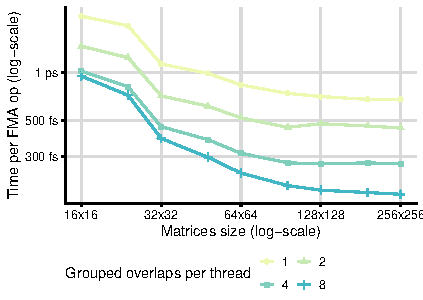
\includegraphics[width=\textwidth]{crosscorr/plots/one-to-one/grouped-overlap.pdf}
		\caption{The \emph{grouped-overlap} results, normalized times (per FMA) for completely saturated GPU}
		\label{fig:grouped-overlap}
	\end{minipage}%
	\begin{minipage}{.03\textwidth}~
	\end{minipage}
	\begin{minipage}{.48\textwidth}
		\centering
		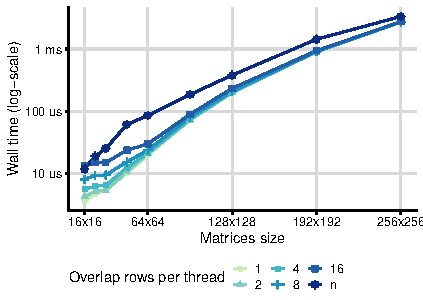
\includegraphics[width=\textwidth]{crosscorr/plots/one-to-one/split-row.pdf}
		\caption{The \emph{split-row} benchmark on various inputs, absolute (wall) times}
		\label{fig:split-row}
	\end{minipage}
\end{figure}

\subsubsection{Fine-grained parallelism}
% \paragraph{\textbf{\emph{split-row}}}

When problem size is not sufficient to saturate the GPU, a fine-grained parallelism is required. One possibility is to employ the \emph{split-row} optimization for the warp-shuffle algorithm, which splits each Hadamard product into multiple independently processed stripes. Figure \ref{fig:split-row} shows the performance for different job granularity levels ranging from the finest job of $1$ row per thread to $n$ (all) per thread (no splitting takes place --- i.e., referring to basic warp-shuffle implementation). As expected, the finest granularity helps the most for the smallest matrices and the speedup over $n$ (baseline) variant progressively diminishes as the input size increases (and thus saturates the GPU without splitting).

%\paragraph{\textbf{\emph{warp-per-overlap}}}
The alternate approach (\emph{warp-per-overlap} algorithm) has no tuning parameters, so we do not provide a separate micro-benchmark for it. The comparison of both algorithms is evaluated in the following.

\subsubsection{Comparison of all one-to-one solutions}
%\paragraph{\textbf{One-to-one optimizations comparison}}

Figure~\ref{fig:one-to-one} (left) summarizes the performance of the discussed one-to-one algorithms. The \emph{baseline} algorithm denotes the na\"{i}ve \emph{overlap-wise} implementation (one thread per one overlap with no data reuse) which we use as a baseline. Algorithms, which have tuning parameters, use their optimal values for given input sizes (as determined in the previous micro-benchmarks).

\begin{figure}[ht]
	\centering
	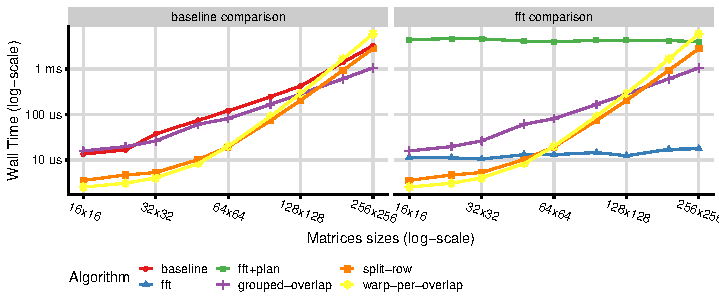
\includegraphics{crosscorr/plots/one-to-one/one-to-one.pdf}
	\caption{Comparison of one-to-one algorithms}
	\label{fig:one-to-one}
\end{figure}

The \emph{grouped-overlap} optimization is the most beneficial for larger matrices while for smaller matrices it suffers the low GPU occupancy due to the insufficient amount of tasks. The \emph{split-row} and \emph{warp-per-overlap} algorithms perform better on smaller matrices as they resolve the occupancy issue. The \emph{warp-per-overlap} performs better on very small inputs as it was designed specifically to prefer core occupancy over data caching. The \emph{split-row} optimization of the \emph{warp-shuffle} algorithm performs slightly worse for matrices smaller than $64\times64$; for larger matrices, the data reuse and coalesced loads become more important, so it outperforms \emph{warp-per-overlap}. Overall, the proposed optimizations perform better than baseline \emph{overlap-wise} algorithm, being $5.3\times$ faster for $16\times16$ input and $3.1\times$ faster for $256\times 256$ input.

% \paragraph{\textbf{Comparison with FFT}}

%Finally, we compare the proposed optimizations against the FFT-based algorithm, in our case the highly optimized CUDA library \emph{cuFFT}~\cite{site:cufft}. Recalling from Section~\ref{sec:cross_corr_fft}, FFT based algorithm must perform the input padding, Discrete Fourier Transform (DFT), Hadamard product, Inverse DFT and quadrant swap. We used cuFFT optimized routines for DFT and Inverse DFT. For Hadamard product, we implemented the custom kernel (Hadamard product is an embarrassingly parallelizable algorithm and its implementation details were omitted for brevity).

%In order to provide less convoluted and fairer results, we decided not to include padding and quadrant swap into the benchmark. We chose to omit the quadrant swap because this step is not generally required for every cross-correlation usecases; e.g., in digital image cross-correlation, only the maximum of the cross-correlation matrix is needed. Skipping quadrant swap therefore makes it more fair comparison with definition-based algorithms. Regarding the paddings, it is a simple operation that may influence the performance very little, so we omitted it for the simplicity of the benchmarking code.

%The DFT routines operate on a \emph{cuFFT plan} --- an opaque data structure, which needs to initialized beforehand. Although we can only speculate what operations does plan initialization exactly performs, cuFFT documentation states that it allocates GPU memory. The allocation takes multiple magnitudes longer than the kernel runtimes, so we decided to plot it separately to provide the better picture of the speedups. We plotted FFT-based algorithms in two variants --- \emph{fft}, which shows the aggregated runtime of DFT, Hadamard product and Inverse DFT, and \emph{fft+plan}, which also adds the plan creation to the sum. Note, that comparing kernel runtimes to memory allocations is not generally fair, but in our case the allocation is an extra step in the FFT algorithm and therfore it is worthy the overall comparison.

The right part of Figure~\ref{fig:one-to-one} reveals that the cuFFT plan creation is the most costly part of the algorithm, dominating the runtime in each measured data point. When the initialization is taken into account, the definition-based approach appears much better in the terms of performance. The turning point, where the \emph{fft+plan} surpasses our optimizations, seems to be around $384\times 384$ matrix. When considering \emph{fft} alone, only the \emph{warp-per-overlap} algorithm outperforms it (having $4.5\times$ speedup on $16\times 16$ inputs) and the turning point is around $48\times 48$.


% -----------------------------------------------------------------------------
\subsection{One-to-many benchmarks}
% -----------------------------------------------------------------------------

The \emph{one-to-many} and \emph{n-to-mn} scenarios enable utilization of the \emph{multi-matrix-right} optimization of the warp shuffle algorithm. This optimization can be combined with \emph{grouped-overlap} or \emph{split-row}, so we present their respective performance evaluation in detail.

We did not include the \emph{warp-per-overlap} evaluation in this section, because it does not provide any additional improvement in terms of performance. The additional workload of multiple cross-correlations mitigates the need for extremely fine-grained parallelism, so the \emph{split-row} optimization is more than sufficient even for the smallest matrices.

\subsubsection{Multi-matrix-right with grouped-overlap}
% \paragraph{\textbf{\emph{multi-matrix-right grouped-overlap}}}

In this configuration, we are benchmarking the one-to-many scenario with $4000$ right matrices, which completely saturates the GPU. The left subplot of Figure~\ref{fig:multimat-right-grouped-overlap} shows the \emph{grouped-overlap} results without the \emph{multi-matrix-right} optimization. In the middle and the right subplot, the number of right matrices per thread is $2$ and $4$ respectively (i.e., enabling the multi-matrix caching). The results indicate that increasing the number of right matrices per thread does not collide with the data reuse made by the \emph{grouped-overlap} optimization and both optimizations can work in synergy.

\begin{figure}[ht]
	\centering
	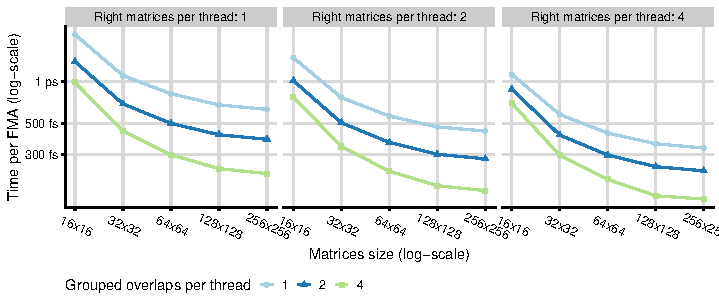
\includegraphics{crosscorr/plots/one-to-many/multimat-right-grouped-overlap.pdf}
	\caption{\emph{Multi-matrix-right}+\emph{grouped-overlap} results (one-to-many, $4000$ right matrices)}
	\label{fig:multimat-right-grouped-overlap}
\end{figure}

Considering a sufficient total number of the right matrices, we can increase the factor of right matrices per thread significantly more and still expect the performance to improve. The primary limitation is the maximum number of registers per thread a GPU allows to allocate. The required number of registers increases linearly with the product of right matrices per thread used by \emph{multi-matrix-right} and warp-wise buffers used by the \emph{grouped-overlap} (which is about $3 \cdot 4^2$ registers per thread for the variant that reuses the data the most intensively in Figure~\ref{fig:multimat-right-grouped-overlap}). When the maximum is exceeded, the GPU resorts to register spilling (offloading to local memory), which harms the performance significantly.

We have observed that the parameter values presented in Figure~\ref{fig:multimat-right-grouped-overlap} are in a reasonable range. Increasing the grouping factor or number of right matrices further does not help much with performance on current GPU architectures, but it creates additional issues with the compilation (especially bloating the size of our artifact). Hence, we have excluded higher values from the presented results for practical reasons.


\subsubsection{Multi-matrix-right with split-row}
% \paragraph{\textbf{\emph{multi-matrix-right split-row}}}

This micro-benchmark was designed to determine how the combination of multi-matrix data reuse and fine-grained parallelism can improve performance. In theory, applying \emph{multi-matrix-right} on small inputs may decrease the performance because it groups tasks, thus limiting the parallelism. Combining multi-matrix optimization with \emph{split-row} may provide enough parallel GPU work whilst improving the data reuse.

\begin{figure}[ht]
	\centering
	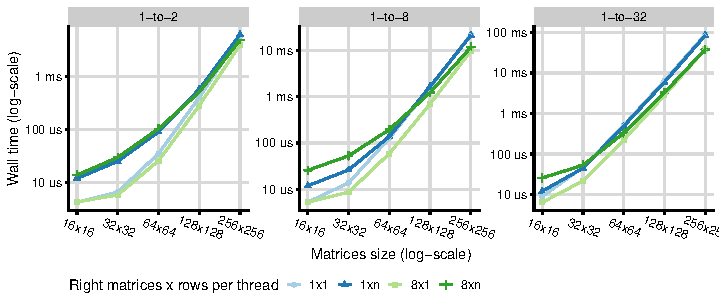
\includegraphics{crosscorr/plots/one-to-many/multimat-right-split-row.pdf}
	\caption{\emph{Multi-matrix-right}+\emph{split-row} benchmark results (please note that the $8\times1$ and $8\times n$ parametrizations are in fact $2\times1$ and $2\times n$ in the \emph{1-to-2} scenario since we can cache only up to the total number of right matrices)}
	\label{fig:multimat-right-split-row}
\end{figure}

%We ploted the optimization combination in Figure~\ref{fig:multimat-right-split-row}. If we compare only \emph{multi-matrix-right} optimization without \emph{split-row} (a triangle and a cross in each subplot), we can see that a big data reuse (cross) decreases the performance for small matrix sizes. But if we look at their \emph{split-row} alternatives (a circle and a square in each subplot), we can see that finer sized jobs counter the performance degradation caused by the data reuse. Ultimately, when the problem size is bigger and a GPU is saturated, these alternatives meet (circles meet with triangles and squares meet with crosses) and the performance is the same.
Figure~\ref{fig:multimat-right-split-row} demonstrates how the \emph{split-row} improves performance for small problem sizes. The $1\times n$ and $8\times n$ denote the versions that do not take advantage of \emph{split-row} (the size of row-stripes is $n$, which stands for the size of the overlapping area). The $1\times 1$ and $8\times 1$ stand for the most fine-grained versions of \emph{split-row} (one task takes only one row). The data indicate that in the extreme, the speedup caused by splitting the rows could reach an order of magnitude ($16\times16$ with a low number of right matrices). Furthermore, the $8\times 1$ parametrization (i.e., the most fine-grained division that caches $8$ right matrices) exhibits the best performance over the examined domain.

\subsubsection{Comparison of one-to-many optimizations}
%\paragraph{\textbf{One-to-many optimizations comparison}}

The overall comparison is presented in Figure~\ref{fig:one-to-many}. Similarly as for one-to-one optimizations, the \emph{split-row} dominates the small matrices and \emph{grouped-overlap} dominates the larger matrices. Employing \emph{multi-matrix-right} (especially when combined with \emph{split-row}) shifts the turning point where higher data reuse wins over more granular jobs. Using $32$ right matrices, we achieve $11.8\times$ speedup over na\"{i}ve \emph{overlap-wise} (baseline) algorithm for $16\times 16$ input and $6\times$ speedup for $256\times 256$ input.

When we compare the best definition-based algorithm with cuFFT, the \emph{split-row} still outperforms \emph{fft} for extra small matrices. The turning point for \emph{fft+plan} is slightly beyond the size of $256\times 256$ for $2$ input matrices, and $128\times 128$ for $32$ input matrices.

\begin{figure}[ht]
	\centering
	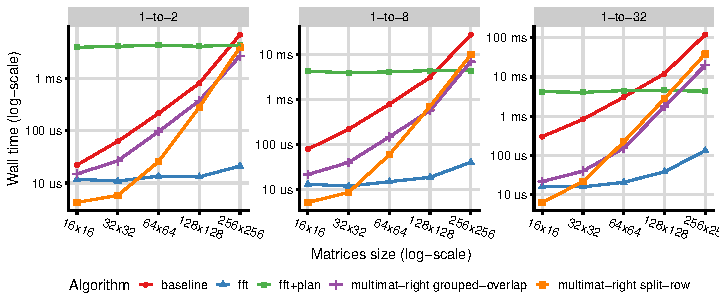
\includegraphics{crosscorr/plots/one-to-many/one-to-many.pdf}
	\caption{Comparison of one-to-many algorithms}
	\label{fig:one-to-many}
\end{figure}


\subsubsection{Extending one-to-many into n-to-mn}

The \emph{n-to-mn} problem is in fact $n$ instances of \emph{one-to-many} problem. There are two ways of extending the \emph{one-to-many} implementation --- we could either simply run the original kernel $n$ times simultaneously or create a new kernel that takes an additional index. After a careful analysis, we found no additional benefits of implementing a separate kernel. When running \emph{one-to-many} kernel $n$ times, the only issue worth mentioning is that the runtime must utilize a sufficient amount of CUDA streams, so the execution of the kernels may overlap in case the individual invocations cannot saturate the GPU.

The overhead of the simultaneous kernel execution is negligible, so we have omitted figures with the performance results from the paper for the sake of brevity. The data and the plots may be found in the attached replication package.


% -----------------------------------------------------------------------------
\subsection{n-to-m benchmarks}
% -----------------------------------------------------------------------------

This scenario allows the most elaborate data reuse pattern called the \emph{multi-matrix-both} optimization. Similarly to \emph{multi-matrix-right}, it can be combined with \emph{grouped-overlap} or \emph{split-row}.

\subsubsection{Multi-matrix-both with grouped-overlap}
%\paragraph{\textbf{\emph{multi-matrix-both grouped-overlap}}}

In Figure~\ref{fig:multimat-both-grouped-overlap}, we present the results of \emph{grouped-overlap} alone (left subfigure), combined with \emph{multi-matrix-right} (center subfigure), and with \emph{multi-matrix-both} (right subfigure). Regardless of the number of grouped overlaps, the \emph{multi-matrix} optimization alone improves the speedup, and the combination of both optimizations exhibits the best performance. In the case of the highest overlap grouping, the speedup of \emph{both} variant over \emph{right} variant is about $1.75\times$ on all input sizes.

\begin{figure}[ht]
	\centering
	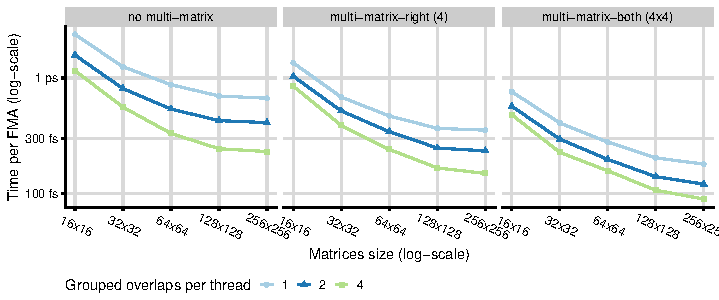
\includegraphics{crosscorr/plots/n-to-m/multimat-both-grouped-overlap.pdf}
	\caption{\emph{Multi-matrix-both}+\emph{grouped-overlap} benchmark results ($128$-to-$128$ matrices)}
	\label{fig:multimat-both-grouped-overlap}
\end{figure}


\subsubsection{Multi-matrix-both with split-row}
%\paragraph{\textbf{\emph{multi-matrix-both split-row}}}

Similarly to \emph{multi-matrix-right} combination, we aim at verifying that \emph{split-row} optimization enables the data reuse on smaller matrices without any performance downgrade. We tested this on two different matrix counts: $2$-to-$2$ and $8$-to-$8$ matrices (top and bottom pair of subfigures in Figure~\ref{fig:multimat-both-split-row} respectively). The results indeed show that for small matrices, the \emph{multi-matrix} alone (the left pair of subfigures) is slower than the \emph{multi-matrix} combined with \emph{split-row} (the right pair of subfigures). The speedup of finer parallelism for $16\times16$ matrix and the highest --- about $5\times$. As expected, the speedup gets negligible for larger matrices.

\begin{figure}[ht]
	\centering
	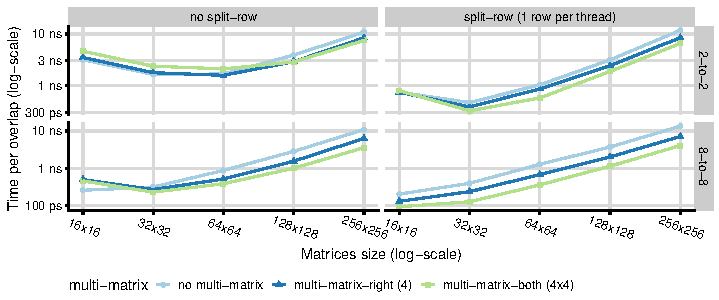
\includegraphics{crosscorr/plots/n-to-m/multimat-both-split-row.pdf}
	\caption{\emph{Multi-matrix-both}+\emph{split-row} benchmark results}
	\label{fig:multimat-both-split-row}
\end{figure}

\subsubsection{Comparison of n-to-m optimizations}
%\paragraph{\textbf{n-to-m optimizations comparison}}

The overall comparison is presented in Figure~\ref{fig:n-to-m}. Similarly to \emph{one-to-many} optimizations, the \emph{split-row} dominates smaller inputs while \emph{grouped-overlap} dominates larger inputs. However, when the multi-matrix factor gets higher ($32$-to-$32$ matrices), the \emph{grouped-overlap} gets more efficient than \emph{split-row} as the GPU is already saturated and data reuse becomes more important.

Another observation is that cuFFT gets better even for slightly smaller matrices when the number of cross-correlations is growing. That is a natural conclusion of the fact that the cuFFT plan initialization takes constant time, so it gets more amortized into the overall computation. For $32$-to-$32$ matrices, the turning point gets as low as $64\times 64$ matrices.

\begin{figure}[ht]
	\centering
	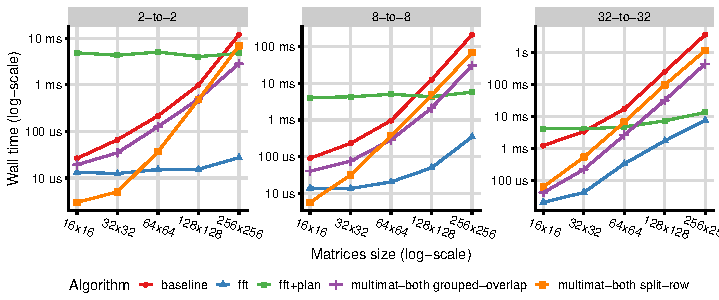
\includegraphics{crosscorr/plots/n-to-m/n-to-m.pdf}
	\caption{Comparison of n-to-m algorithms on various inputs.}
	\label{fig:n-to-m}
\end{figure}


% -----------------------------------------------------------------------------
\subsection{Summary and outcomes}
% -----------------------------------------------------------------------------

To summarize the empirical results, we provide basic guidelines for selecting the optimal algorithm and its optimization. Table~\ref{tab:overview-all} presents the algorithm of choice for given scenarios (rows) and matrix sizes (columns). The \emph{one-to-many} instances implicitly assume utilization of \emph{multi-matrix-right} optimization and the \emph{n-to-m} always employ \emph{multi-matrix-both} optimization.

As indicated in the previous benchmarks, the smallest configurations benefit from \emph{split-row} optimization (or the \emph{warp-per-overlap} algorithm, in case of \emph{one-to-one} scenario). The middle-sized problems can benefit from the \emph{grouped-overlap} optimization and the largest problems should switch to the FFT-based approach which is asymptotically better.

Please note that the turning points for each configuration are not exact and they may differ slightly across the GPU architectures.

\begin{table}
	\begin{tabular}{l|cccccccc}\toprule
		             & $16^2$                                     & $32^2$                                & $64^2$                                & $128^2$         & $192^2$                     & $256^2$ & $384^2$ & $\infty$ \\\midrule
		\emph{1-to-1}   & \multicolumn{3}{c|}{\texttt{warp-overlap}} & \multicolumn{1}{c|}{\texttt{split}}   & \multicolumn{3}{c|}{\texttt{grouped}} & \multicolumn{1}{r}{\texttt{fft+p}}                                \\\bottomrule
		\emph{1-to-2}   & \multicolumn{4}{c|}{\texttt{split}}        & \multicolumn{2}{c|}{\texttt{grouped}} & \multicolumn{2}{c}{\texttt{fft+p}}                                                                        \\
		\emph{1-to-8}   & \multicolumn{3}{c|}{\texttt{split}}        & \multicolumn{2}{c|}{\texttt{grouped}} & \multicolumn{3}{c}{\texttt{fft+p}}                                                                        \\
		\emph{1-to-32}  & \multicolumn{2}{c|}{\texttt{split}}        & \multicolumn{2}{c|}{\texttt{grouped}} & \multicolumn{4}{c}{\texttt{fft+p}}                                                                        \\\bottomrule
		\emph{2-to-2}   & \multicolumn{4}{c|}{\texttt{split}}        & \multicolumn{2}{c|}{\texttt{grouped}} & \multicolumn{2}{c}{\texttt{fft+p}}                                                                        \\
		\emph{8-to-8}   & \multicolumn{3}{c|}{\texttt{split}}        & \multicolumn{2}{c|}{\texttt{grouped}} & \multicolumn{3}{c}{\texttt{fft+p}}                                                                        \\
		\emph{32-to-32} & \multicolumn{4}{c|}{\texttt{grouped}}      & \multicolumn{4}{c}{\texttt{fft+p}}                                                                                                                \\\bottomrule
	\end{tabular}
	\centering
	\caption{Overview of the best algorithms (and optimizations) for individual scenarios and input sizes}
	\label{tab:overview-all}
\end{table}

\section{Related Work}\label{sec:crosscorr_relwork}

% Projit nize uvedene a dat je nejak do perspektivy pripadne chronologicke navaznosti
% Same as with the previously mentioned work, these approaches solve a slightly different problem with regards to data reuse since they share the intermediate results between workers, while we reuse only the global memory loads. But the idea of grouping multiple overlaps into a single job is the same.

% There are plenty of other scientific papers related to GPU cross-correlation~. However, they describe GPU optimizations for a specific scientific use-case and use almost exclusively some modifications of the asymptotically better FFT-based algorithms. Therefore, the optimizations mentioned in these works are not applicable to our problem.

% unsorted
% --------

% general template matching
% 2d cross correlation implemented using FFT
% \cite{liu2011gpu} - Gpu accelerated fourier cross correlation computation and its application in template matching

% Optical coherence tomography
% 2d
% used in ophtalmology, where detailed imagery of the retina, the optic nerve, and other parts of the eye is essential for accurate diagnosis 
% \cite{Kapinchev2015} - GPU implementation of cross-correlation for image generation in real time

% particle image velocimetry - CC is used to compute displacement vectors
% process has high complexity and is optimized using GPU cuFFT
% \cite{zeng2022gpu} - PU-accelerated MART and concurrent cross-correlation for tomographic PIV (2022, asi aplikacni)

% Digital image correlateion
% 2d
% \cite{zhang2015} - High accuracy digital image correlation powered by GPU-based parallel computing

% seismic:
% --------------

% ambient noise imaging uses noise CC functions to obtain earth underground structures
% due to increasing number of seismomenters and the data they produce, getting more accurate earth's seismic information is limited by the runtime of NCF
% authors optimize it on GPU 
% \cite{zhou2021high} - A High Performance Computing Method for Noise Cross-Correlation Functions of Seismic Data

% another seismic usecase for GPU cross correlation
% \cite{beauce2017fast} - Fast Matched Filter (FMF): An Efficient Seismic Matched‐Filter Search for Both CPU and GPU Architectures

% PCC is used for Interstation correlation, which is the basic operation in seismic noise and coda-wave interferometry
% PCC has high computational complexity, authors rewrite it in terms of complex FFT and provide GPU impl
% \cite{ventosa2019towards} - Towards the processing of large data volumes with phase cross-correlation (2019, aplikacni)

% stereo vision:
% ---------------

% authors introduce optimized algorithms and provide real-time GPU implementation of disparity map computation used in autonomous vehicle applications
% 2d
% \cite{fan2017real} - Real-time implementation of stereo vision based on optimised normalised cross-correlation and propagated search range on a gpu (2017, aplikacni)
% \cite{syed2021accelerated} - Accelerated Stereo Vision Using Nvidia Jetson and Intel AVX
% \cite{chang2022efficient} - Efficient stereo matching on embedded GPUs with zero-means cross correlation

% astronomy:
% ----------

% signal processing for radio astronomy
% % 1d
% \cite{Clark2011} - Accelerating Radio Astronomy Cross-Correlation with Graphics Processing Units
% \cite{ord2015murchison} - The Murchison widefield array correlator
% \cite{ragoomundun2020cublas} - A cuBLAS-based GPU correlation engine for a low-frequency radio telescope

% Many works leverage some form of partitioning cross-correlation problem into tasks to be executed in parallel. Khalil et al.~\cite{khalil2013accelerating} distributes the work of 1D cross-correlation between nodes in a local network. The sequence of all delays (overlaps in our terminology) is `sliced' and distributed according to the number of nodes and their computing power. In our work, we employ the same distribution technique but with a difference of much finer granularity, dividing work into single overlaps or even into parts of overlaps between workers.

Cross-correlation relates to the problem of signal processing in many different fields and we have collected several examples where the GPU processing creates an edge. In the domain of radio astronomy, all signals from radio antennas need to be usually correlated with each other, which puts this problem in the HPC domain. Various cross-correlation optimizations have been proposed: Clark et al.~\cite{Clark2011} developed a GPU kernel, which promotes tiling and optimized memory transfer. By utilizing both FPGAs and GPUs, Ord et al.~\cite{ord2015murchison} propose a hybrid approach to achieve sufficient performance. Ragoomundun et al.~\cite{ragoomundun2020cublas} utilize batched matrix multiply routines of the cuBLAS GPU library to implement their optimized correlator to enable real-time processing for telescopes.

Seismic interferometry is another use case, where cross-correlation plays a major role. An increasing amount of seismometers allows the production of more detailed seismic information of the Earth but it is typically limited by the processing runtime. Zhou et al.~\cite{zhou2021high} optimize noise cross-correlation functions used to obtain Earth's underground structures. Ventosa et al.~\cite{ventosa2019towards} implement a GPU version of phase cross-correlation, which is used in Interstation correlation. Beaucé et al.~\cite{beauce2017fast} discuss optimizations of Fast Matched Filter, which is an important tool in the detection of seismic events.

Applications of cross-correlation can be also found in computer vision. Fan et al. discuss autonomous vehicle applications in the context of disparity maps~\cite{fan2017real} (used for stereo vision) or lane detection~\cite{fan2018real}. Typically, mobile platforms such as autonomous cars and robots have strict limits to their power intake, so Syed et al.~\cite{syed2021accelerated} and Chang et al~\cite{chang2022efficient} described ways to further optimize stereo vision algorithms on embedded hardware, such as Nvidia Jetson GPU, to achieve the required speed of processing while maintaining low power consumption.

It has been established that fast cross-correlation is useful in various practical domains. However, most of the papers mentioned in the previous put little effort into the optimizations of the algorithm and provide only straightforward GPU implementations. We would like to introduce also several works which have influenced our proposed solution. Perhaps the most fundamental is the well-known BLAS library called Magma~\cite{tomov2011magma}. It is one of the first libraries that effectively utilized two-level tile caching (shared memory and registers) in matrix multiplication.

Similar caching can be employed when image tiles are being compared many times. An example of an algorithm that relies heavily on comparing image tiles is Block-matching and 3D denoising, which has a very efficient CUDA implementation by Honzátko et al.~\cite{paper:krulis_3d_block}. Similarly to cross-correlation, the BM3D algorithm searches for similarity between image parts, so it compares different overlapping tiles. In the CUDA implementation, the authors made an observation that the overlapping work can be computed only once and re-used. They also employed an efficient work distribution pattern where an entire warp cooperates on a comparison of a single patch. Closer to our research, a CUDA-accelerated implementation of 3D stereo vision~\cite{Cui2019Real} employs cross-correlation computed on neighborhoods of all pixels to determine relative shifts between images taken from stereo cameras. The implementation of the 3D vision was quite efficient thanks to effective caching in shared memory, albeit it was implemented for a rather specific Nvidia Jetson TX2 device.

We found no elaborate optimizations directly for the cross-correlation, but more thorough research was done in the domain of convolution, especially in methods related to training neural networks. Yan et al.~\cite{yan2020optimizing} presented an optimized GPU implementation for batched Winograd convolutions. Similarly to us, they have observed the low arithmetic density of their solution and attempted to mitigate the problem by cleverly caching the data in the registers. The solution presented by Lu et al.~\cite{lu2021optimizing} introduces even more complex optimizations. In particular, they employ warp-wise buffers managed by warp-shuffle instructions and data reuse patterns similar (but simpler) to our grouped-overlap optimization. However, the convolution algorithms optimize for larger input on one side and rather small filter on the other side, so it is not directly applicable for general cross-correlation.

The work that inspired our design probably the most was the CUDA implementation of Levenshtein's edit distance~\cite{paper:levenstein}. It uses circular warp-wise buffers and clever utilization of warp-shuffle instructions that lead to a very efficient algorithm that is quite fast despite the unavoidable data dependencies inherent to the Levenshtein. It also uses double buffering to promote coalesced loads, similar to our left-matrix buffers.

Finally, there is one aspect of modern GPUs that we have not focused on in our work. Contemporary NVIDIA architectures since Volta incorporate \emph{Tensor units} in the GPU streaming multiprocessors. These units are specifically designed to perform fused multiply-add instructions (FMA), which are essential in many computations including cross-correlation. The tricky part is to use them efficiently since they are designed only for particular combinations of FMAs that are used in neural networks. Kikuchi et al.~\cite{kikuchi2022calculation} presented an implementation specifically tailored for the use of CUDA tensor cores. They employ \emph{Warp Matrix Multiply-Accumulate API} to compute multiple waveform pairs with multiple shifts (overlaps) simultaneously. The solution is claimed to achieve better performance than cuBLAS, but it is applicable only for 1D cross-correlation. A similar idea was proposed by Yamaguchi et al.~\cite{Yamaguchi2019} earlier, but they have focused on half-precision (FP16) computations. The FMA optimizations were omitted from our paper for the sake of brevity, but they definitely present another possibility to achieve even better performance.


% pre kazdy bod v lavom obrazku sa vytvori window 9x9 a ten sa posuva po y osi v pravom obrazku. pre kazdy posun sa vypocita CC s pravym obrazkom. zo vsetkych posunov pre dany zdrojovy bod sa vyberie najvyssia hodnota CC a ta sa ulozi do vysledneho obrazku
% impl: thread block je definovany ako w x h thredov. kazdy thread pocita jeden pixel vysledneho obrazkudo
% do shared mem sa nacita (w+8) x (h+8) dat z laveho obrazku - kazdy thread teda ma vsetky data, ktore potrebuje
% nasledne sa spravi nieco ako (w+8) x (h+8) hadamard produkt a potom si kazdy thread urobi horizontalnu a vertikalnu sumaciu a ziska CC pre svoj pixel
% ziaden data reuse vramci roznych posunov (kazdy posun sa pocita osobitne)
% kedze okno je mensie ako obrazky, niektore overlapy nezdielaju iba data (ako je u nas) ale aj samotne nasobenia (co u nas uz neplati)
% z pohladu reusovania nasobeni su na tom asi tak dobre ako to je mozne, jedina zdvojena praca je na hranciach thread blokov
% ale z pohladu reusovania nacitanych dat je to bieda, napr z dovodu pocitania posunov osobitne
%\cite{Cui2019Real} - Real-Time Stereo Vision Implementation on Nvidia Jetson TX2

% konvolucia
% je tam nieco ako nas warp-buffer a nieco ako nas grouped-overlap
% autori cielili na optimalizaciu pre male filtre (3x3, 5x5) a claimuju 2x zrychlenie oproti cudnn
% 1. optimalizacia: (buffer)
% autori zvolili thread per "overlap" (per jednu konvoluciu) - zistili, ze ked mas 2 susedne posuny 5x5 filtru, tak kazdy riadok ma overlap v 4 elementoch
% pre 5x5 to vyriesili tak, ze kazdy thread si nacita 1. a 5. element a pomocou shfl_xor si docita zvysne 3 elementy (2. 3. a 4.) - takze kazdy thread ma reg buffer velkosti 5
% ale na to aby si v shfl_xor indexoval ten buffer statickymi indexami (a teda dovolil compileru ho ulozit v registroch), tak musis pred kazdym shfl urobit nieco ako 
% shfl_var = (laneid == sth) ? first_element_in_buffer : last_element_in_buffer; shfl_xor(shfl_var, 2); (oni to nerobili cez ternarny operator)
% podporu vacsieho fitra ako 5x5 docielili tak, ze fitler nxn rozsekali na filre nx5 bez zmeny zmieneneho postupu
% to znamena, ze dve stvorice threadov pracujuce na susednych castiach jedneho filtra uz nebenefituju ziaden data reuse
% zhrnutie s velkou mierou domyslania: 
% v prvom kroku warp nacita 32 consecutive input elementov zacinajuc na adrese A, v druhom kroku nacitaju 32 elementov na adrese A+5
% dalej nastavaju 3 warp shuffle, nakoniec si kazdy thread naplni svoj 5miestny buffer spravnymi elementami z input matice
% a nakoniec sa ide pocitat 5 FMA instrukcii pre kazdy thread
% nacitavanie filtru nie je zmienene - ale vieme, ze je v shared mem
% 2. optimalizacia: (grouped-overlap)
% ak nie sme uplne v prvom riadku vstupnej matice, tak ten 5miestny buffer kontribuuje v niekolkych konvoluciach susednych na y-ovej osi
% autori tento nacitany buffer nasobia potencialne az so vsetkymi riadkami filtra 
% zhrnutie: podobne, ako nas grouped-overlap, ale data reuse je len na "lavej" strane, filter sa musi nacitat duplicitne
% \cite{lu2021optimizing} - Optimizing depthwise separable convolution operations on gpus


% modifikovana konvolucia pre inspiraciu - boj s nizkou aritmetickou intenzitou rieseny cachovanim dat v registroch
% \cite{yan2020optimizing} - Optimizing batched winograd convolution on GPUs

% TOHLE NA ZAVER - kam by se to dalo jeste rozsirit (pouziti FMA)
% pouzivaju tensor cores + shared memory ako "buffer"
% CUDA API nedefinuje ako je fragment matice pre tensor operaciu rozlozeny v registroch - existuje len volanie load_matrix_sync, ktore to hodi do opaque typu fragment
% optimalizacia: uhadnem rozlozenie fragmentu v registroch - vdaka tomu nemusim vykonstruovat fragment ako suvisly blok pamate (potrebny pre load_matrix_sync), ale mozem vyzobat fragment zo shared priamo do registrov
% je to 1d cross-correlation, takze "pravu maticu" by slo rotovat medzi registrami na rovnakom principe ako nas warp-sized buffer - v praci ale pouzivaju len shared mem 
% input je zda sa one-to-many (zvycajne 1:16 s 1024 timesteps) - presnejsie - mame 16 "template waves" dlzky 256 a jeden observation dlzky 1024, z ktoreho berieme okno dlzky 256 korelujeme ho s kazdym template wave
% zhruba pomer global loads ku tensor operaciam je 1:12 a shared loads ku tensor operaciam je 1:4
% kod: https://github.com/nlnxfkl/TC-enhanced_Cross-correlation_Function/blob/main/compdef_gpu.cu - pozor, pisal to fortranista
% vysledky ukazuju dosiahnutie 34% teoretickeho maxima TFLOPS - A100 ma 19.5 TFLOPS FP32 (obyc) a 156 TFLOPS TF32 (tensor)
% my mame pri 1x8 one-to-many 0.1 TFMAPS (tera FMA za s) pre 16x16 a 5.03 TFMAPS pre 256x256, co je nieco ako 25% ak 1FMA=1FLOP (1x32 pre 256x256 sa posuvame na 7.89 TFMAPS, 32x32 pre 256x256 je to 9.7)
%Kikuchi et al.~\cite{kikuchi2022calculation} use CUDA tensor cores to calculate cross-correlation of time-series data. They use Warp Matrix Multiply-Accumulate API to compute multiple waweform pairs with multiple time shifts simultaniously. In our terminology, this corresponds to computing multiple overlaps of multiple matrix pairs. This approach proves to provide high performance, as authors state to achieve greater FLOPs than using cuBLAS, but it is applicable only to 1D cross-correlation data.


%\cite{Yamaguchi2019} % to iste ako Kikuchi, ale s FP16 (kikuchi to citoval)


\section{Conclusions}\label{sec:crosscorr_conclusions}

We have proposed a novel approach to definition-based implementation of cross-correlation for contemporary GPUs. The proposed algorithm takes advantage of the data reuse principle --- i.e., the operations are rearranged so that every value loaded into a register is used multiple times. This way, the load operations from global memory are reduced significantly, which leads to overall performance improvement. To extend this idea further, we designed a data-exchange schema where the values in registers are shuffled among neighboring threads using warp-shuffle instructions, which are much faster than loads from global memory and measurably faster than shared memory. We have also experimented with different scenarios when multiple (shared) input matrices are cross-correlated simultaneously, which enables another level of parallelism and data reuse. The optimizations presented in this paper can lead to a speedup that exceeds an order of magnitude with respect to na\"{i}ve (baseline) CUDA implementation.

We have also compared our algorithms with a traditional FFT approach. As expected, in the case of small matrices, the definition-based approach significantly outperforms the cuFFT implementation due to the costly initialization and preprocessing phase of the FFT transform. In the case of \emph{one-to-one} correlation, the \emph{warp-shuffle} algorithm is better even for $256\times 256$ matrices. When multiple matrices are correlated (the \emph{n-to-m} scenario), the turning point is roughly at the size of $64\times 64$. The proposed algorithms are also available (along with many other implementations we experimented with) as source codes provided in the attached replication package, so our conclusions may be independently verified and the code may be easily adapted for immediate application.


% \section*{Acknowledgements}

% This paper was supported by Charles University institutional funding SVV 260698/2023.








%%
%% The "title" command has an optional parameter,
%% allowing the author to define a "short title" to be used in page headers.
\chapter{GPU-acceleration of neighborhood-based dimensionality reduction algorithm EmbedSOM}

%%
%% The "author" command and its associated commands are used to define
%% the authors and their affiliations.
%% Of note is the shared affiliation of the first two authors, and the
%% "authornote" and "authornotemark" commands
%% used to denote shared contribution to the research.
% \author{Adam Šmelko}
% \email{smelko@d3s.mff.cuni.cz}
% \orcid{0000-0001-8334-2783}
% \author{Martin Kruliš}
% \email{krulis@d3s.mff.cuni.cz}
% \orcid{0000-0002-0985-8949}
% \author{Jiří Klepl}
% \email{klepl@d3s.mff.cuni.cz}
% \orcid{0000-0002-2231-4073}
% \affiliation{%
%   \institution{Department of Distributed and Dependable Systems, Charles University}
%   \city{Prague}
%   \country{Czechia}
% }


% \keywords{Dimensionality reduction, Single-cell cytometry, GPU acceleration, CUDA, kNN, Optimizations}


\section{Introduction\label{sec:intro}}

Dimensionality reduction algorithms emerged as indispensable utilities that enable various forms of intuitive data visualization, providing insight that in turn simplifies rigorous data analysis.
The development has benefited especially the life sciences, where algorithms like t-SNE~\cite{maaten2008visualizing} reshaped the accepted ways of interpreting many kinds of measurements, such as genes, single-cell phenotypes and development pathways, and behavioral patterns~\cite{toghi2019quantitative,cande2018optogenetic}.

The performance of the non-linear dimensionality reduction algorithms becomes a concern if the analysis pipeline is required to scale or when the results are required in a limited amount of time such as in clinical settings.
To tackle the limitations of poor scalability, Kratochvíl et al. developed EmbedSOM~\cite{kratochvil2019generalized}, a dimensionality reduction and visualization algorithm based on self-organizing maps (SOMs)~\cite{kohonen1990self}.
EmbedSOM provided a $10\times$ speedup on datasets typical for single-cell cytometry data visualization while retaining the competitive quality of the results.
Still, the parallelization potential of EmbedSOM remained mostly untapped as of yet.

This paper describes an efficient, highly parallel GPU implementation of EmbedSOM designed to provide real-time results on large datasets. The implementation is accompanied by performance benchmarks of individual optimizations to evaluate the optimal variants for different dataset sizes. Both the implementation and the empirical data are available in our GitHub repository\footnote{\url{https://github.com/asmelko/gpgpu24-artifact}}.

In the paper, we first describe the EmbedSOM algorithm in Section~\ref{sec:methods}. We specifically detail the CUDA-based GPU implementation of the algorithm in Section~\ref{sec:impl} and evaluate its performance in Section~\ref{sec:results}. Related work is discussed in Section~\ref{sec:embedsom_relwork} and Section~\ref{sec:outro} concludes the paper.

% Dimensionality reduction algorithms emerged as indispensable utilities that enable various forms of intuitive data visualization, providing insight that in turn simplifies rigorous data analysis.
% Various algorithms have been proposed for graphs and high-dimensional point-cloud data, and many different types of datasets that can be represented with a graph structure or embedded into vector spaces.
% The development has benefited especially the life sciences, where algorithms like t-SNE~\cite{maaten2008visualizing} reshaped the accepted ways of interpreting many kinds of measurements, such as genes, single-cell phenotypes and development pathways, and behavioral patterns~\cite{toghi2019quantitative,cande2018optogenetic}.

% The performance of the non-linear dimensionality reduction algorithms becomes a concern if the analysis pipeline is required to scale or when the results are required in a limited amount of time such as in clinical settings.
% The most popular methods, typically based on neighborhood embedding computed by stochastic descent, force-based layouting or neural autoencoders, reach applicability limits when the dataset size is too large.
% To tackle the limitations, we have previously developed EmbedSOM~\cite{kratochvil2019generalized}, a dimensionality reduction and visualization algorithm based on self-organizing maps (SOMs)~\cite{kohonen1990self}.
% EmbedSOM provided an order-of-magnitude speedup on datasets typical for single-cell cytometry data visualization while retaining the competitive quality of the results.
% The concept has proven useful for interactive and high-performance workflows in cytometry~\cite{kratochvil2020shinysom,kratochvil2020gigasom}, and easily applies to many other types of datasets.
% Despite that, the parallelization potential of the extremely data-regular design of EmbedSOM algorithm has remained mostly untapped.

% Our contribution in this paper is a natural continuation of the development:
% We describe an efficient, highly parallel GPU implementation of EmbedSOM designed to provide interactive results on large datasets.
% The implementation is sufficiently fast to provide real-time visualizations of datasets larger than $10^5$ of individual data points on off-the-shelf hardware, while maintaining smooth video-like frame rate.
% We demonstrate that the result gives unprecedented, controllable view of the details of specific high-dimensional datasets.
% The instant feedback available to the user opens possibilities for partial supervision of the visualization process, allowing user-intuitive resolution of possible visualization ambiguities as well as natural exploration of new datasets.
% We demonstrate some of the achievable results on two realistic datasets.
% The resulting software, called \emph{BlosSOM}, is published as free and open source.
% BlosSOM can be readily utilized to reproduce our results and explore more datasets; additionally it contains support for working with data formats (mainly, the FCS standard~\cite{fcs}) that make it immediately useful for visualization of existing and new biological data.

% In the paper, we briefly describe the EmbedSOM algorithm (Section~\ref{ssec:embedsom}), and show an extension of its generalized form that dynamically mixes the user feedback to the learning process, thus enabling the semi-supervised learning (Section~\ref{ssec:dynamic}).
% We specifically detail the CUDA-based GPU implementation of the algorithm in Section~\ref{sec:impl}, and report the achieved performance improvements (Section~\ref{ssec:perf}).
% Finally, we showcase the achievable results on biological data, and discuss possible future enhancements and applications that would aid data analysis (Sections~\ref{ssec:appl}, \ref{ssec:future}).

\section{Landmark-directed dimensionality reduction\label{sec:methods}}

EmbedSOM is a visualization-oriented method of non-linear dimensionality reduction that works by describing a high-dimensional point by its location relative to landmarks equipped with a topology and reproducing the point in a low-dimensional space using an explicit low-dimensional projection of the landmarks with the same topology~\cite{kratochvil2019generalized}.
% The ability to effectively work with a simplified model of the data differentiates it from other dimensionality reduction methods; in turn it offers superior performance by reducing the amount of necessary computation as well as by opening parallelization potential, since the computations of the projections of many individual points are independent.
% In the setting of flow and mass cytometry data visualization, this provided speedup of several orders of magnitude against the other available methods~\cite{kratochvil2020gigasom,kratochvil2020shinysom}.

% While the EmbedSOM originally used the (eponymous) self-organizing maps to find the viable high- and low-dimensional manifolds from the data points, the concept generalized well to many other methods.
% In particular, the projection has been shown to work with any (even random) set of high-dimensional landmarks that have the low-dimensional counterparts organized by any selected dimensionality reduction method (which may be slow in comparison, given the fact that the set of landmarks is usually small).
% In Section~\ref{ssec:dynamic}, we utilize this freedom of model specification to provide dynamic view of the dataset, based on a simplified dataset model that the user may refines in order to improve the dataset view.

More formally, the EmbedSOM algorithm works as follows. Let $d$ be the dimension of the high-dimensional space and assume $\mathbb{R}^2$ is the low-dimensional space for brevity. EmbedSOM processes $n$ $d$-dimensional points in a matrix $X$ of size $n\times d$, and outputs $n$ 2-dimensional points in matrix $x$ of size $n\times 2$.
The high- and low-dimensional landmarks similarly form matrices $L$ of size $g\times d$ and $l$ of size $g\times 2$, where usually $g\ll n$.
Each point $X_i$ is transformed to a point $x_i$ as:
\begin{enumerate}
\item $k$ nearest landmarks are found for point $X_i$ ($k$ is a constant parameter satisfying $3\leq k\leq g$)
\item the landmarks are ordered and a score is assigned to each of them, using a smooth function of the distance that assigns the highest score to the closest landmark and $0$ to the $k$-th landmark (this ensures the smoothness of projection in cases when $k<g$ \cite{kratochvil2019generalized})
\item for each pair $(u,v)$ of the closest $k-1$ landmarks (i.e., the ones with non-zero score), a projection of the point $X_i$ is found on the 1-dimensional affine space with coordinate 0 at $L_u$ and 1 at $L_v$; the 1-dimensional coordinate of the projection in this affine space is taken as $D_{uv}(X_i)$ and the same projected coordinates are defined in the low-dimensional space as $d_{uv}(x_i)$
\item point $x_i$ is fitted to the low-dimensional space so that the squared error in the coordinates weighed by nearest-landmark scores ($s_u, s_v$) is minimized: $$x_i = \argmin_{p\in \mathbb{R}^2} \sum_{u,v}s_u\cdot s_v\cdot \left(D_{uv}(X_i)-d_{uv}(p)\right)^2$$
\end{enumerate}

Because $d_{uv}(p)$ is designed as a linear operator, the error minimization problem (step 4) collapses to a trivial solution of $2$ linear equations with $2$ variables.
A complete algorithm may be found in the original publication~\cite[Algorithm 1]{kratochvil2019generalized}.

% Efficient implementation of the EmbedSOM algorithm is the main performance concern that enables its interactive use.
% The original CPU-based parallel implementation was able to visualize hundreds of thousands of points per second on common use-cases.
% As a major result of this paper, in Section~\ref{sec:impl} we improve this performance to the scale of milliseconds, enabling real-time projection and rendering of points based on interactive control of the high- and low-dimensional landmarks.

% \subsection{User supervision and model interaction}
% \label{ssec:dynamic}

% EmbedSOM landmarks (the matrices $L$ and $l$) represent a simplified dataset model that can be used to conveniently and predictably steer the dimensionality reduction.
% In particular, the main property of the projection --- visualizing the data points from the neighborhood of a landmark $L_i$ preferably in the neighborhood of the corresponding low-dimensional $l_i$ --- gives an intuitive interpretation for the landmark positions:
% Manipulating the high-dimensional landmarks chooses which data are visualized, while manipulating the low-dimensional landmarks chooses the desired location of the visualized points.
% Smoothness of the projection then grants that the smooth manipulations of the landmarks that will result in smooth changes of the results, enabling predictable user control and refinement.

% However, positioning of the landmarks in the high-dimensional space (which is inherently complicated to navigate) and finding a suitable layout of the landmarks in the low-dimensional space is an overly complicated task for the user alone.
% The main concern of this section is to design a simplification of the control of the landmarks, so that viable results may be reached in an automated way and the user interaction is required only for decisions that can not be decided automatically such as resolving dimensionality-reduction ambiguities and positioning of the dataset parts that matches some assumed semantics.
% We describe two ways of automated and user-controlled positioning of the landmarks that implement this kind of partial supervision, thus making the method semi-supervised.
% Both are roughly based on the embedding methods proposed in previous work~\cite{kratochvil2019generalized}; only modified for interactive environment.

% The main tasks that the user supervision interface has to resolve are thus as follows:
% \begin{itemize}
% \item place the landmarks to viable positions in the high-dimensional space
% \item dynamically increase or decrease the resolution of the model in specified places, by adding or removing landmarks
% \item organize low-dimensional landmarks to reflect the structure in the high-dimensional space, while allowing the user to resolve ambiguities that arise in dimensionality reduction
% \item react to the changes in the input datasets, such as scaling of the dimensions and appearance of new points
% \end{itemize}

% \begin{figure}
% \centering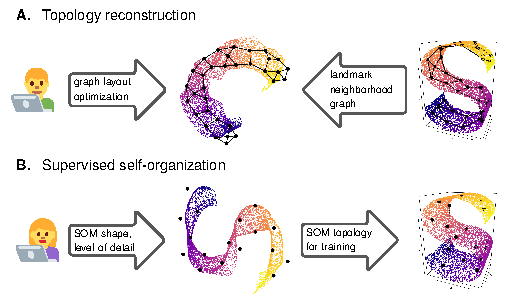
\includegraphics[width=\linewidth]{embedsom/pic/sup.pdf}
% \caption{
% Schema of the 2 implemented user supervision approaches.
% The user interacts with low-dimensional model that is intuitive to navigate, and indirectly drives the positioning of the corresponding high-dimensional image of the model, using either a graph-based approach (Section~\ref{sssec:sup-graph}) or self-organizing map approach (Section~\ref{sssec:sup-som}).
% }
% \label{fig:supervis}
% \end{figure}

% The two methods detailed below are briefly illustrated in Figure~\ref{fig:supervis}.

% \subsubsection{Semi-supervised structure reconstruction}
% \label{sssec:sup-graph}

% One possible approach to position the high-dimensional landmarks is to sample them randomly from the distribution of the original data set, and position the low-dimensional ones to reflect the structure of the sampling.
% In the original unsupervised implementation, we used a random sample of the input dataset as the landmark positions, and a dimensionality reduction methods such as t-SNE to position the landmarks.
% Importantly, the positioning of low-dimensional landmarks could be performed relatively quickly even by rather time-demanding algorithms such as t-SNE, because the algorithm only had to work with the highly reduced version of the dataset in landmarks.

% In the dynamic, supervised context, we need to avoid the randomness in order to avoid flickering in the view of the dataset, and utilize a dimensionality reduction algorithm that may reflect the user input.
% Thus, we chose to continuously run an interactive version of $k$-means clustering with a low learning rate to find good $k$ high-dimensional landmarks $L$, and employ a simple force-based graph layouting algorithm on a neighborhood graph of $L$ to embed the landmarks to 2D.
% Both these algorithms are capable of smooth transitions between consecutive states, thus avoiding the flicker.
% Moreover, force-based graph layouting may be intuitively steered by the user by dragging the graph nodes. Similarly, the points may be added and removed from $k$-means clustering in the same interface in order to increase and decrease the model resolution.

% Addition of a new landmark is implemented as follows: The user selects a low-dimensional landmark, and upon pressing a special button, both the low-dimensional landmark and its high-dimensional counterparts are duplicated in their respective spaces.
% The $k$-means algorithm then consecutively optimizes the positions of the landmarks to provide a detailed view.
% This stability of the result is helped by the initialization properties of $k$-means where the cluster centroids tend to stay in the same clusters~\cite{franti2019much} (counter-intuitively, the same properties have an undesirable impact on the robustness of unsupervised clustering).
% Most importantly, this enables the user to position new landmarks without having to navigate the possibly overwhelming complexity of the data distribution in the high-dimensional space.

% \subsubsection{Supervised training of self-organizing maps}
% \label{sssec:sup-som}

% Alternatively, the user may choose a SOM approach as originally intended for EmbedSOM.
% BlosSOM supports user drawing of the 2-dimensional version of the SOM on a canvas, which is used as-is as the low-dimensional landmarks.
% New landmarks may be added at any position, as their initial high-dimensional coordinates can be fitted using the coordinates of the other close landmarks in 2D.

% The positioning of the landmarks in 2D is then used as a topology for training the high-dimensional landmarks as neuron weights of the SOM algorithm.
% To extend the supervision possibilities of this step, BlosSOM adds specific controls that allow the user to manually sweep through the SOM neighborhood sizes and learning rates (usually labeled $\sigma$ and $\alpha$ \cite{kohonen1990self}), which is done automatically in unsupervised SOM training.
% This allows the users to optionally pause the SOM training at any stage and fix or customize the SOM topology at coarse detail level (with larger $\sigma$) before it is used to train fine details (small $\sigma$, the difference is closer detailed in Figure~\ref{fig:somsigma}).

% \begin{figure}
% \centering
% \begin{tikzpicture}[node distance=1em]
% \node (a) {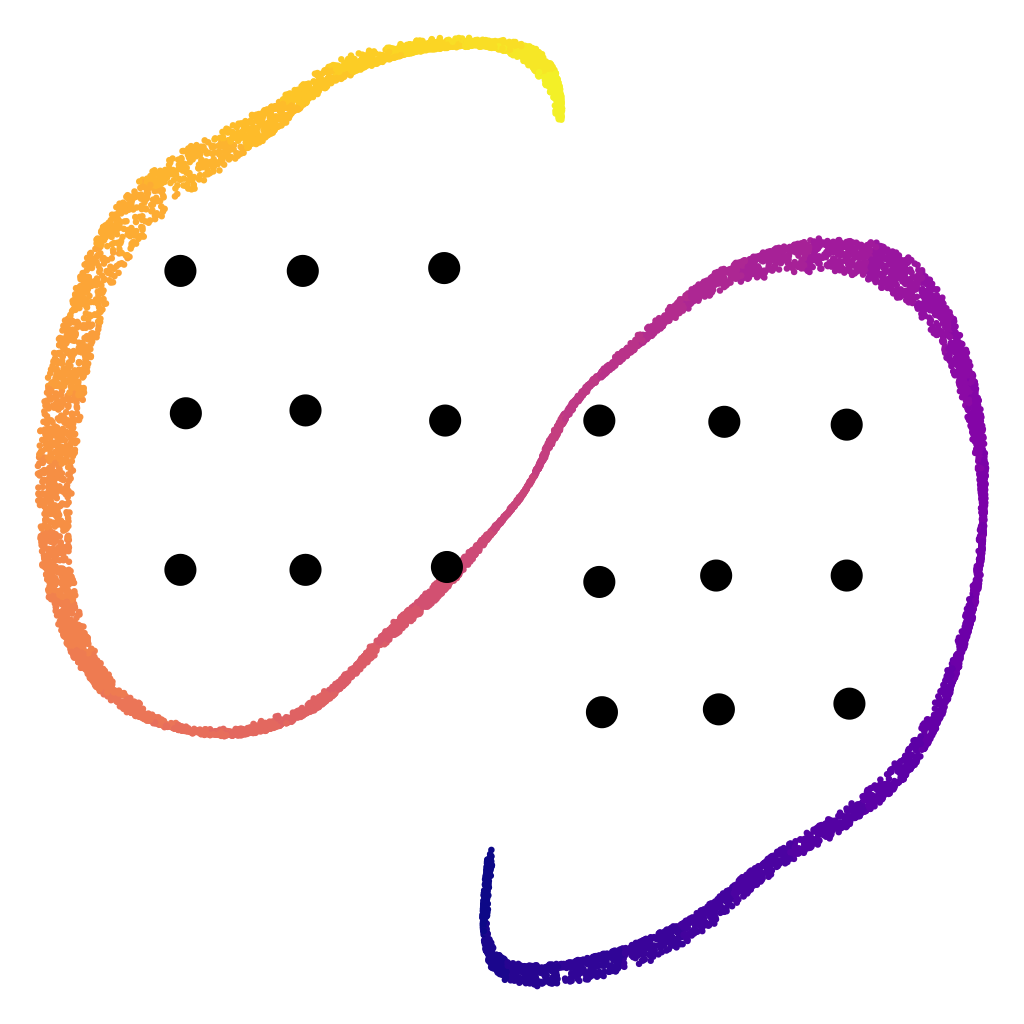
\includegraphics[width=.25\linewidth]{embedsom/pic/S_begin_2d.png}};
% \node[right=of a] (b) {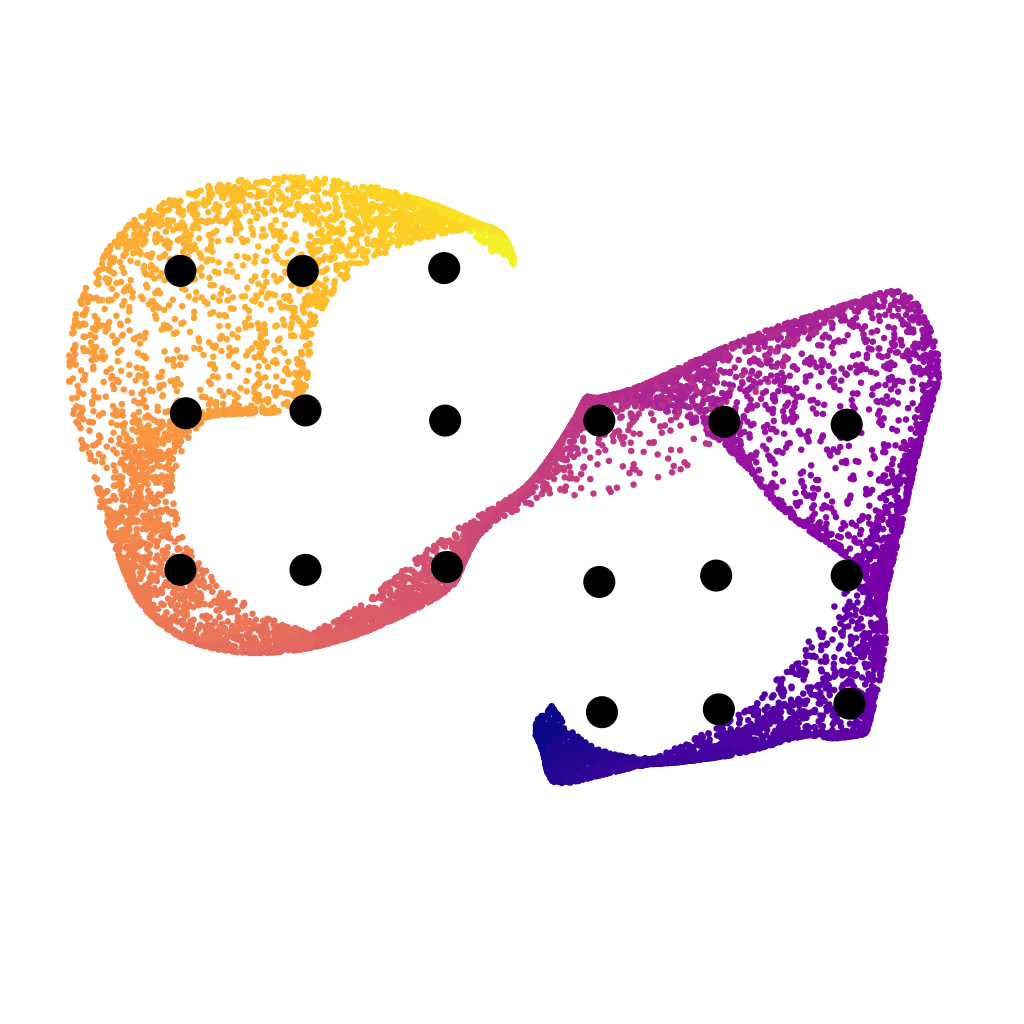
\includegraphics[width=.25\linewidth]{embedsom/pic/S_mid_2d.png}};
% \node[right=of b] (c) {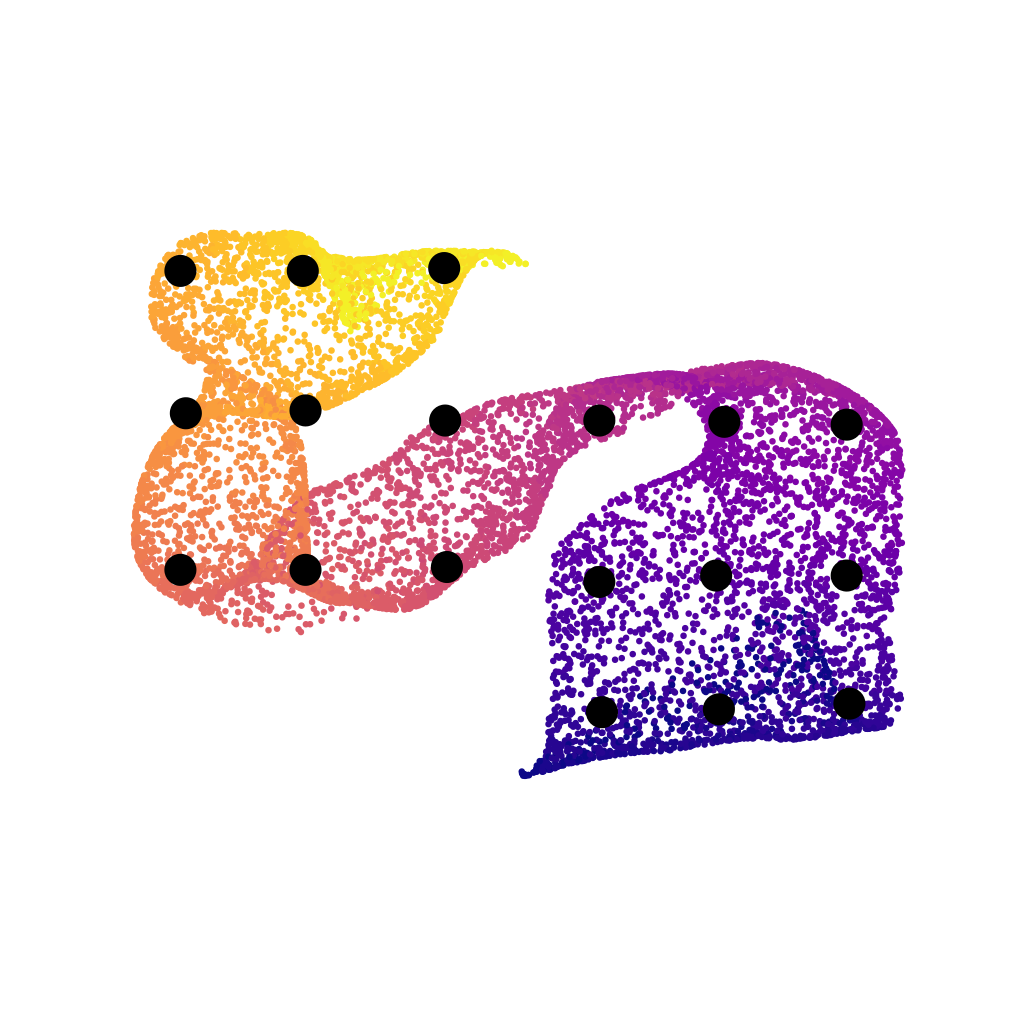
\includegraphics[width=.25\linewidth]{embedsom/pic/S_end_2d.png}};
% \node[below=0pt of a] {$\sigma=1.5$};
% \node[below=0pt of b] {$\sigma=0.8$};
% \node[below=0pt of c] {$\sigma=0.2$};
% \end{tikzpicture}
% \caption{
% Effect of different settings of $\sigma$ SOM training parameter on the output detail, demonstrated on an extruded S-shaped 3D dataset and a custom SOM shape.
% Value of $\sigma$ decreases from left to right, progressively revealing finer details but losing larger-scale structure.
% }
% \label{fig:somsigma}
% \end{figure}

\section{GPU implementation of EmbedSOM}\label{sec:impl}

While EmbedSOM is relatively straightforward to parallelize for mainstream CPU architectures, several challenges appear when designing of an optimal implementation for contemporary GPUs.
In this section, we outline the key optimizations that allowed us to run the high-performance dimensionality reduction in EmbedSOM, and give an overview of the relative performance gains achieved by the algorithm choice.

Technically, the algorithm consists of two main parts that provide distinct implementation challenges:

\begin{itemize}
\item {\bfseries $k$-NN step}\quad
The search of $k$-nearest landmarks in $L$ for each data point from $X$ requires a highly irregular selection of indices of $k$ lowest values from columns of the dynamically computed distance matrix $L^T\cdot X$.

\item {\bfseries Projection step}\quad
Computation of the small linear system that is used to find the minimal-error-projection of a point, namely of projections $D_{uv}$ and the derivatives $\frac{\delta d_{uv}}{\delta x_i}$ (Section~\ref{sec:methods}), is difficult to optimize due to irregular memory access patterns of collecting the data for the computation.
\end{itemize}

% We carried out the implementation in NVIDIA CUDA~\cite{guide2013cuda}, the performance validation presented in the next sections is accordingly carried out only on NVIDIA hardware that supports CUDA.
% Despite our benchmarks being NVIDIA-specific, the presented kernels do not depend on any NVIDIA-specific functionality, and the results should be portable to other GPU programming frameworks (such as Vulkan Compute shaders) and hardware of other vendors.
% We expect that only minor adjustments will be required to compensate for GPU design differences, such as the 64-thread wavefronts on AMD devices.

In the following two sections, we describe in detail the optimizations of the CUDA implementation.

\subsection{$k$-NN selection step}\label{sec:impl-knn}

The task of the first part of the algorithm is to find $k$ nearest landmarks (from $L$) for every data point in $X$.
This comprises two sub-steps: computing Euclidean distances for every pair from $L$ and $X$ and performing point-wise reduction that selects a set of $k$ nearest landmarks for each of the $n$ points, based on the computed distances.

While the Euclidean distance computation is mathematically simple and embarrassingly parallel, achieving optimal throughput on GPUs is quite challenging~\cite{krulivs2017employing}.
In particular, the ratio between the data transfers and the arithmetic operations performed by each GPU core is heavily biased towards data transfers.
The overhead of data transfers is best prevented by finding a good caching pattern for the input data that is able to optimally utilize all hardware caches (L1 and L2), shared memory, and core registers.

The parallel implementation of the $k$-nearest neighbors search is even more challenging.
The $k$-NN problem is computed individually for each data point, which provides the space for possible parallelization.
However, concurrently processed instances of a na\"{i}ve $k$-NN implementation exhibit severe code divergence because the selection process is purely data-driven, and requires a high amount of memory allocated per core.
Optimally, the $k$-NN selection is realized by customized versions of parallel sorting algorithms, which are well-researched and possess existing GPU implementations~\cite{singh2018survey}.

Our implementation chooses to optimize both sub-steps since the ratio of the amount of required computations can be easily biased by the configuration of parameters $d$ and $k$.
In particular, processing high-dimensional datasets with a low $k$ parameter spends significantly more time in the distance computation, but lower-dimensional datasets with higher $k$ require more time in the nearest neighbor selection.

Concerning the perspective of software design, the implementation may use separate kernels for both sub-tasks or a single fused kernel.
Kernel separation provides better code modularity and much flexibility in work-to-thread division and data caching strategy, at the cost of having to materialize all the computed distances in the GPU global memory, thus significantly increasing the total amount of data transfers.
Contrary to that, a fused kernel may immediately utilize the computed distances in $k$-NN computation without transferring the data to global memory and interleaving the distance computations with $k$-NN may help to improve the ratio between computations and data transfers.
Since our initial observations showed that the overhead of the data transfers required for kernel communication is relatively high, we decided to implement only the fused variant for the sake of simplicity.
The usage of separate kernels might be interesting in the future, especially for extreme values of $d$ that diminish the relative cost of the distance data transfer.

\subsubsection{Available algorithms for $k$-NN}

There are many approaches to $k$-NN selection, varying in complexity and parameter-dependent performance. We implemented several of the possibilities (as described in this section) to substantiate our choice of the algorithm for GPU EmbedSOM.

As a baseline (labeled \Alg{Base}), we used the most straightforward approach to GPU parallelization which simply invokes original sequential code for every data point concurrently.
The \alg{Base} kernel is spawned in $n$ threads (one for each data point), and each thread computes the distance between its data point and all landmarks while maintaining an ordered array of $k$ nearest neighbors.
The array is updated by an insert-sort step performed for every new computed distance --- i.e., by starting at the end of the array and moving the new distance-index pair towards smaller values until it reaches the correct position.

\Alg{Shared} algorithm is a modified version of the baseline algorithm that utilizes shared memory as a cache, following the recommended optimization practice of improving performance by caching data that are reused multiple times~\cite{guide2013cuda}.
In this case, we cache the landmark coordinates, which are sufficiently small to fit in the shared memory for all tested parametrizations.

In \Alg{GridInsert} algorithm, we utilize the shared memory to cache both landmarks and points.
However, the limited size of shared memory imposes limitations of the amount of cached data. Hence, the algorithm was parametrized by the block height $h$ (number of cached points from $X$) and the block width $w$ (number of cached landmarks from $L$).
The algorithm runs in epochs, each of which first caches $h$ points and $w$ landmarks, and then computes $h \cdot w$ distance values using only data in shared memory.
While the distances are computed concurrently by the whole thread block, we chose to avoid explicit synchronization in the $k$-NN step, using only $h$ threads to incorporate the newly computed distances into $h$ separate $k$-NN results using the insert-sort steps.
The \alg{GridInsert} should achieve better throughput in the distance computation thanks to the caching, at the cost of slightly sub-optimal $k$-NN reduction; thus, giving the best performance on high-dimensional datasets and low values of $k$.

% The above algorithms focus solely on optimizing the distance computation; we further detail the possible optimizations of the $k$-NN selection.

% A straightforward way for computing the $k$ nearest neighbors in parallel is to sort an entire array of distances using a parallel sorting algorithm, then taking the first $k$ items.
% Although the overhead of storing the distances might be excessive, we expected the strategy to be competitive especially for large values of $k$ (approaching the total number of landmarks in the grid).
% We use this approach in \Alg{Radix} algorithm, which employs the highly-optimized sorting algorithm from the state-of-art CUB library~\cite{cub}.
% The algorithm allocates an entire thread block to process one input data point.
% The block cooperates on computing the Euclidean distances by dividing the landmarks evenly among the threads.
% The distances are stored along with indices in the shared memory block, which is then sorted by the CUB radix sort, and subsequently the first $k$ items are copied to the result buffer in global memory.
% Importantly, the whole block of $g$ distance-index pairs must fit in the shared memory, which imposes a limitation on the maximal amount of landmarks, and prevents much of the input caching in the shared memory, impacting the efficiency of distance computation.

Finally, improvising on our previous work~\cite{krulivs2015optimizing}, we implemented \Alg{Bitonic} $k$-NN selection algorithm, which utilizes routines from the highly parallelizable bitonic sorting algorithm.
Bitonic sorting is very suitable for parallel lockstep execution~\cite{krulivs2017employing}, and the capability to merge sorted sequences has allowed us to keep only $2k$ distances (instead of $g$) in the shared memory.
This method benchmarked the best on the average, so it is selected as default for EmbedSOM and we describe it more thoroughly in the following.


\subsubsection{Bitonic approach to $k$-NN}

The \alg{Bitonic} approach can be seen as a combination of the benefits of the other algorithms: It does not require materializing all distances in the memory to do a full sort and even though it does not use an elaborate input caching strategy like \alg{GridInsert}, it still gives interesting results because the data loading operations can be partially overlapped with bitonic sorting operations if enough warps are allocated to one streaming multiprocessor.

\begin{figure}
	\centering
	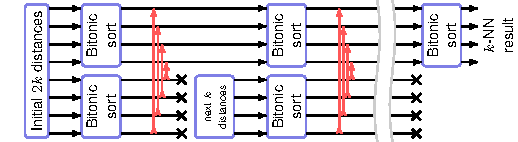
\includegraphics{embedsom/pic/bitonic.pdf}
	\caption{\alg{Bitonic} algorithm for $k$-NN selection ($k=4$). Each horizontal line represents a data item in the shared memory. Red lines represent comparators ensuring, that the intermediate $k$ `best' neighbors and in the top buffer.}
	\label{fig:bitonic-schema}
\end{figure}

The bitonic comparator network provides a building block that, given two buffers of size $k$ of neighbor distances sorted by bitonic sort, selects the closest $k$ of the neighbors in a single (parallel) operation, allowing us to quickly discard neighbors that do not belong into the $k$-neighborhood.
Applying this operation iteratively on $k$-sized blocks of distances sorted by the bitonic sort (as shown in Figure~\ref{fig:bitonic-schema}), we obtain a highly performing scheme that requires only $2k$ items present in the shared memory.
In particular, the shared memory always contains a $k$-block of distances (and corresponding indexes) that holds $k$ so-far-nearest neighbors, and one block of $k$ distances that are computed from $L$; in each iteration, both blocks are sorted by the bitonic sorter in parallel and merged by the bitonic comparator to move the distances of new nearest $k$ neighbors into the intermediate block.
The other block is then re-filled by a new set of $k$ distances from $L$.

Technically, each step of the sorting net requires $\frac{k}{2}$ comparators, thus optimally $\frac{k}{2}$ threads that work concurrently on the $h$-sized block.
Hence, we allocate $k$ threads for each data point, which alternate their work between computing a block of $k$ distances and performing two bitonic sorts on two $k$-sized blocks in parallel.
For simplicity, our implementation assumes that $k$ is always a power of $2$, and excessive output of the sorter is discarded.



\subsection{Projection step}\label{sec:impl-projection}

The second part of the dimensionality reduction method is the actual projection into the low-dimensional space.
The computation of the low-dimensional point position $x_i$ by EmbedSOM involves: 
(1) Conversion of the distances collected in the $k$-NN to scores;
(2) Orthogonal projection of $X_i$ to $k \choose 2$ lines generated by the $k$ neighbors to create contributions to the final approximation matrix;
(3) Solution of the resulting small linear system using Cramer's rule.

Since the first and the last steps are embarrassingly parallel problems with straightforward optimal implementation and since the second step is the most time demanding (performing $\mathcal{O}(k^2)$ operations on vectors of size $d$), we focus mainly on the orthogonal projections. Its computation is complicated by a highly irregular pattern of repeated accesses to an arbitrary $k$-size subset of $L$. We designed several algorithms that successively optimize the access patterns, detailed below.

The baseline algorithm \Alg{Base} uses the most straightforward parallel approach (similar to \alg{Base} $k$-NN), where each thread computes the projection of one single point sequentially so the concurrency is achieved only by processing multiple points simultaneously.
All data are stored in the global memory, and no explicit cache control is performed.

The irregular repeated access to the elements of $L$ hinders the performance of the baseline algorithm.
In the \Alg{Shared} algorithm, we chose to reorganize the workload so that each projection is computed by a whole block of threads that cooperatively iterate over the landmark pairs.
As a result, the input data of the orthogonal projection (i.e., the $k$ nearest neighbors from $L$ together with the distances, scores, and 2D versions of the landmarks) can be cached in shared memory.
The intermediate sub-results represented by $2\times3$ matrices are successively added into privatized copies of each thread to avoid explicit synchronization and aggregated at the end using a standard parallel reduction, enhanced with warp-shuffle instructions (a similar scheme is used in optimal CUDA k-means implementation~\cite{krulis2020detailed}).

Because the data transfers comprise a considerable portion of the \alg{Shared} algorithm execution time, we have optimized the transfers using alignment and data packing techniques, yielding the \Alg{Aligned} algorithm.
The implementation is based on using vector data types (e.g. \texttt{float4} in CUDA) to enable utilization of $128$-bit load/store instructions, which improves overall data throughput.
The vectorization comes only at a relatively small cost of aligning and padding the vectors to $16$-byte blocks.

\begin{figure}
\centering
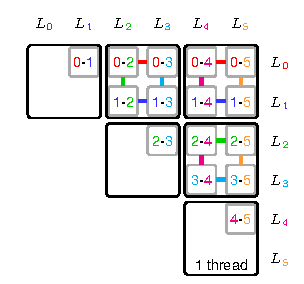
\includegraphics{embedsom/pic/reg-caching.pdf}
\caption{Detail of the caching of landmark data in \alg{Registers} projection kernel. Multiple landmark pairs (small boxes) are processed by each thread (large boxes). Caching of the landmark data in registers allows the reuse of loaded data (color lines), thus reducing the amount of memory accesses.}
\label{fig:proj}
\end{figure}

To further improve the data caching, we implemented algorithm \Alg{Registers}, where each thread computes more than one landmark pair in a single iteration so that the coordinates loaded into its registers can be shared as inputs among multiple landmark-pairs computations.
The data sharing scheme is detailed in Figure~\ref{fig:proj}.
We found that it is optimal to group the threads into small blocks of $2\times2$ computation items, saving half of the data loads.
Larger groups are theoretically possible, but even $3\times3$ caused excessive registry pressure and impaired performance on contemporary GPUs.
The innermost loop of the algorithm iterates over $d$ so that only a single \texttt{float4} value per each landmark is kept in registers.


\section{Experimental Results}\label{sec:results}

The main objective of the benchmarking was to measure the speedups achieved by different applied optimizations and to determine the optimal algorithms and their parameter setting for the sub-tasks of EmbedSOM computation.

The timing results, presented in the following sections, were collected as kernel execution times measured by a standard system high-precision clock. Each test was repeated $10\times$ and the mean values are presented in the subsequent figures. The relative standard deviations of the measurements were less than $5\%$ so we chose not to include them. Complete measurements are available in our GitHub repository\footnote{\url{https://github.com/asmelko/gpgpu24-artifact}}.

Results were collected on NVIDIA Tesla A100~PCIe~80~GB running CUDA 12.2. All benchmarking datasets were synthetic, containing exactly $1$Mi points ($n=2^{20}$, reflecting the common sizing of real-world datasets~\cite{adan2017flow}) with all coordinates sampled randomly from the same uniform distribution.
The performance of the benchmarked algorithms is not data-dependent, except for the case of caching performance in the projection step, where the completely random dataset is the worst-case scenario.


\subsection{Performance of $k$-NN selection}\label{sec:knn-evaluation}

Here we give an overview of performance and viable parameter settings observed for the $k$-NN selection algorithms.

Notably, all algorithms for $k$-NN are affected by CUDA thread block sizing which affects warp scheduling and data reuse possibilities of the shared-memory cache.
We observed that the total thread block size of $256$ threads was either optimal or near to optimal for almost all tested configurations, except for \alg{GridInsert} that performed the best with $64$ threads for lower values of $d$ and $g$ parameters.

Parameters $w$ and $h$\footnote{Technically, parameter $h$ is determined by the thread block size divided by $w$, we thus optimize only $w$.} of the \alg{GridInsert} algorithm determine the ratio between data transfers and computations, but may also affect the pressure on the shared memory.
Empirical evaluation indicates that the algorithm performs the best when each parallel insertion sort is performed in a separate warp, so the code divergence in SIMT execution is prevented (i.e., $w$ is a multiple of $32$)
The optimal performance was observed for $w$ equal to $96$ or $128$; However, the speedup over $w=32$ is relatively low.

\begin{figure}
	\centering
	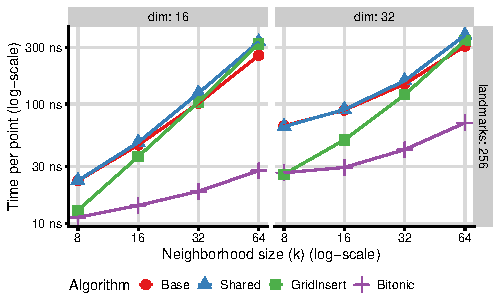
\includegraphics{embedsom/final-plots/algs_knn_repre_ampere.pdf}
	\caption{Amortized performance of $k$-NN step for a single input point using parameters usual in flow cytometry}
	\label{fig:knn-result-repre}
\end{figure}

A comparison of the best parametrizations of each algorithm on various configurations common in our target use cases is shown in Figure~\ref{fig:knn-result-repre}.
The \alg{Bitonic} algorithm significantly outperformed the other algorithms.
The speedup of \alg{Bitonic} over \alg{Base} was between $3\times$ to $20\times$ and usually more than $2\times$ over the second-ranking method.

The benchmarking also confirmed a rather huge scaling difference between algorithms based on divergent insertion sort and algorithms based on sub-quadratic parallelizable sorting schemes.
We conclude that despite the simplicity that might enable GPU speedups in certain situations, the insertion sort is too slow for larger values of $k$ in this case.

As an interesting result, we observed that despite following the general recommendations, the straightforward use of shared memory (in the \alg{Shared} algorithm) did not improve overall performance over the \alg{Base}.
Quite conversely, the overhead of explicit caching even caused a slight decrease in the overall performance.

% \begin{figure}
% 	\centering
% 	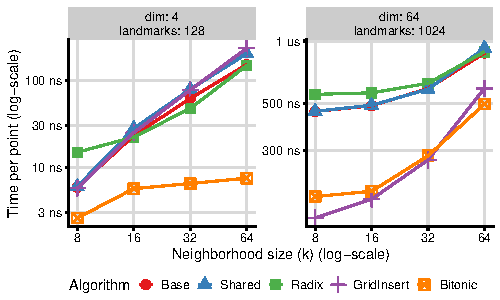
\includegraphics{embedsom/final-plots/algs_knn_extreme_ampere.pdf}
% 	\caption{Amortized $k$-NN step performance in corner-case parametrizations}
% 	\label{fig:knn-result-extreme}
% \end{figure}

We additionally report the performance measurements for two selected corner cases with extreme values of $g$ and $d$ (figure omitted due to the page limit).
Mainly, the total volume of the computation required to prepare the Euclidean distances scales with $g\cdot d$, which becomes dominant when both are maximized.
At that point, we observed that \alg{GridInsert} provides comparable or mildly better performance than \alg{Bitonic}, especially in cases where $k$ is small and the overhead of insertion sorting is not as pronounced.

Naturally, we should ask whether it could be feasible to combine the benchmarked benefits of \alg{GridInsert} and \alg{Bitonic} algorithms in order to get the best of both approaches (optimal inputs caching and fast $k$-NN filtering).
While an investigation of this possibility could be intriguing, we observed that a fused algorithm would require very complicated management of the shared memory (which both algorithms utilize heavily), and the estimated improvement of performance was not sufficient to substantiate this overhead; we thus left the question open for future research.


\subsection{Performance of projection step}

% \begin{figure}
% 	\centering
% 	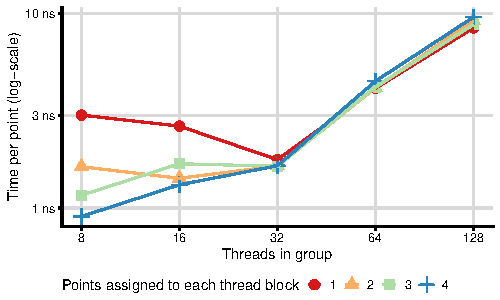
\includegraphics{embedsom/final-plots/proj_multi_block_ampere}
% 	\caption{Comparison of various sizes and numbers of thread groups in the \alg{Shared} projection algorithm in the extreme parametrization ($k = 8, d = 4$).}
% 	\label{fig:multi_block}
% \end{figure}

\begin{figure}
	\centering
	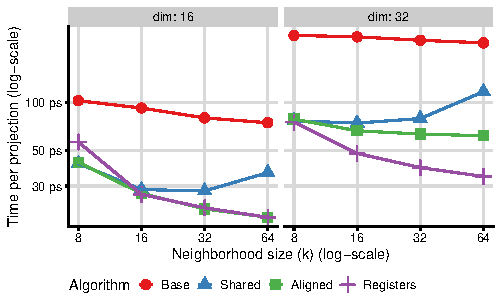
\includegraphics{embedsom/final-plots/algs_proj_repre_ampere}
	\caption{Amortized performance of a single projection operation in the algorithms that compute the projection step (showing the most important problem parametrizations)}
	\label{fig:proj_repre}
\end{figure}

The projection algorithms described in the previous section have only two execution parameters:
The size of the CUDA thread block and the number of data points assigned to a thread block (threads are divided among the points evenly).
We observed that selecting more than one point per thread block is beneficial only in the case of relatively small problem instances (low $k$ and $d$) because it prevents underutilization of the cores.

The optimal size of the CUDA thread blocks depends mainly on the parameters $k$ and $d$.
In case of \alg{Shared} algorithm, optimal values ranged from $32$ (for $k=8$, $d=4$) to $64$ ($k=d=64$).
With the caching optimizations in \alg{Aligned} and \alg{Registers}, the optimal thread block size was slightly higher, reaching $128$ for the most complex problem instances.
We assume this is a direct consequence of the improved memory access efficiency which gives space for parallel execution of additional arithmetic operations.

Figure~\ref{fig:proj_repre} shows the performance of the best algorithm configurations for the representative parametrizations.
All three algorithms perform almost equally for small $k$, giving around $3\times$ speedup over \alg{Base}.
The importance of optimizations in \alg{Aligned} and \alg{Registers} grows steadily when parameter $k$ increases, up to around $10\times$ speedup at $k=64$.
In conclusion, the optimal algorithm for the EmbedSOM projection is determined by the dimensionality of the dataset --- \alg{Registers} performs better at higher dimensions ($d\geq32$) while \alg{Aligned} was slightly better for lower dimensions.


\subsection{Complete algorithm}\label{sec:impl-complete}

A complete GPU implementation of the EmbedSOM algorithm is the combination of the best implementations of $k$-NN and projection steps.
The selected algorithms \alg{Bitonic} and \alg{Registers} are simply executed sequentially on large blocks of $X$, sharing only a single data exchange buffer for transferring the $k$-NN data.
Notably, since the data exchange between the algorithm parts is minimal, comprising only distances and neighbor indexes from the $k$-NN selection, we claim that no specific optimizations of the interface are required.

% Because of the relative complexity of the methods, we did not attempt to compute a theoretically possible data processing throughput.
% On the other hand, the collected results seem to scale proportionately to the asymptotic time complexities of the algorithms, roughly following $\mathcal{O}(n\cdot d\cdot g\cdot \log_2 k)$ for the $k$-NN and $\mathcal{O}(n\cdot d \cdot k^2)$ for the projection.
% That gives an optimistic outlook on the future scalability of the implementation, especially because the larger problem instances bear no additional overhead.

\begin{figure}
	\centering
	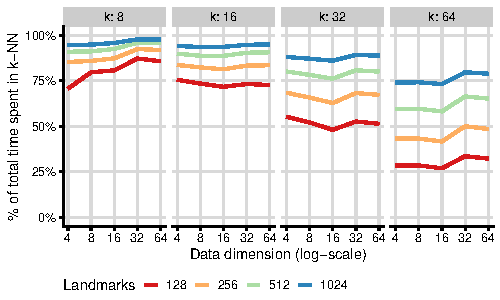
\includegraphics{embedsom/final-plots/esom_percent_ampere}
	\caption{The relative time spent by the $k$-NN computation usually dominates the execution of GPU EmbedSOM, composed of \alg{Bitonic}+\alg{Registers} algorithms.
  Projection computation time becomes dominant only for relatively impractical parametrizations of low $g$ and high $k$.}
	\label{fig:proj_percent}
\end{figure}

Finally, we highlight the relative computation complexity of both steps (Figure~\ref{fig:proj_percent}), which changes dynamically with $k$ and might be viable as a guide for further optimization.
We observed that for common parametrizations ($k\simeq 20$, $g\simeq 500$), most of the computation time is spent in $k$-NN step, and projection performance becomes problematic only in cases of almost impractically high $k$.
The results align with the asymptotic time complexities of the algorithms, roughly following $\mathcal{O}(n\cdot d\cdot g\cdot \log_2 k)$ for the $k$-NN and $\mathcal{O}(n\cdot d \cdot k^2)$ for the projection.

% The performance might be further improved by spatial indexing methods or approximate neighborhood selection algorithms, but we are currently not aware of a scheme that could provide a decisive performance improvement over the optimized brute-force neighbor processing~\cite{krulis2020detailed}.


\section{Related work}\label{sec:embedsom_relwork}

% In this work, we specifically reflect the needs of many areas of life sciences where large multidimensional point-cloud-like datasets occur, such as population biology, microscopy imaging, metagenomics, and others.

% Single-cell cytometry~\cite{adan2017flow} forms a canonical example of this niche: The recent development of hardware and measuring equipment has enabled a precise collection of multiple features of each of millions of cells in a sample. Clinicians and biologists commonly measure metrics such as protein expression on the cell surface using antibody-based markers. For instance, the marker detection may be performed optically by exciting fluorochromes with a laser and measuring emission spectra or using a specific binding of heavy metal ions detected by mass spectrometry techniques such as time-of-flight~\cite{spitzer2016mass}. Both methods allow cheap acquisition of data about more than 50 selected features at once, typically with several million single-cell measurements from each sample~\cite{vanikova2021omip,rodriguez2020systems}. Additionally, the development of single-cell sequencing methods has enabled to sequence the mRNA present in the individual cells~\cite{ziegenhain2017comparative}, typically yielding a dataset with thousands of data points of dimensions higher than $10^4$.

% Due to the variability in the samples, data, and measurements, analyzing and interpreting the results is challenging. Biologists usually analyze the datasets by linearly projecting the features to 2-dimensional plots and manually selecting the cells of interest in a process called gating~\cite{bashashati2009survey}. While computationally simple and easily interpretable by humans, gating gets extremely error-prone as the dimensionality of the dataset increases. It does not provide good support for detecting dataset features of dimensionality higher than $2$, such as complicated pathways and loops in cell phenotypes. Similarly, applying algorithms for clustering analysis provided good detection of cell phenotype clusters but minimal reliability in pathway-style feature detection~\cite{saelens2018comparison}.

% \begin{figure}
% \centering
% {\linewidth=21pc
% \begin{tikzpicture}[font=\tiny\sffamily\bfseries, inner sep=1pt]
% \node[inner sep=0, anchor=south west] (img) at (0,0) {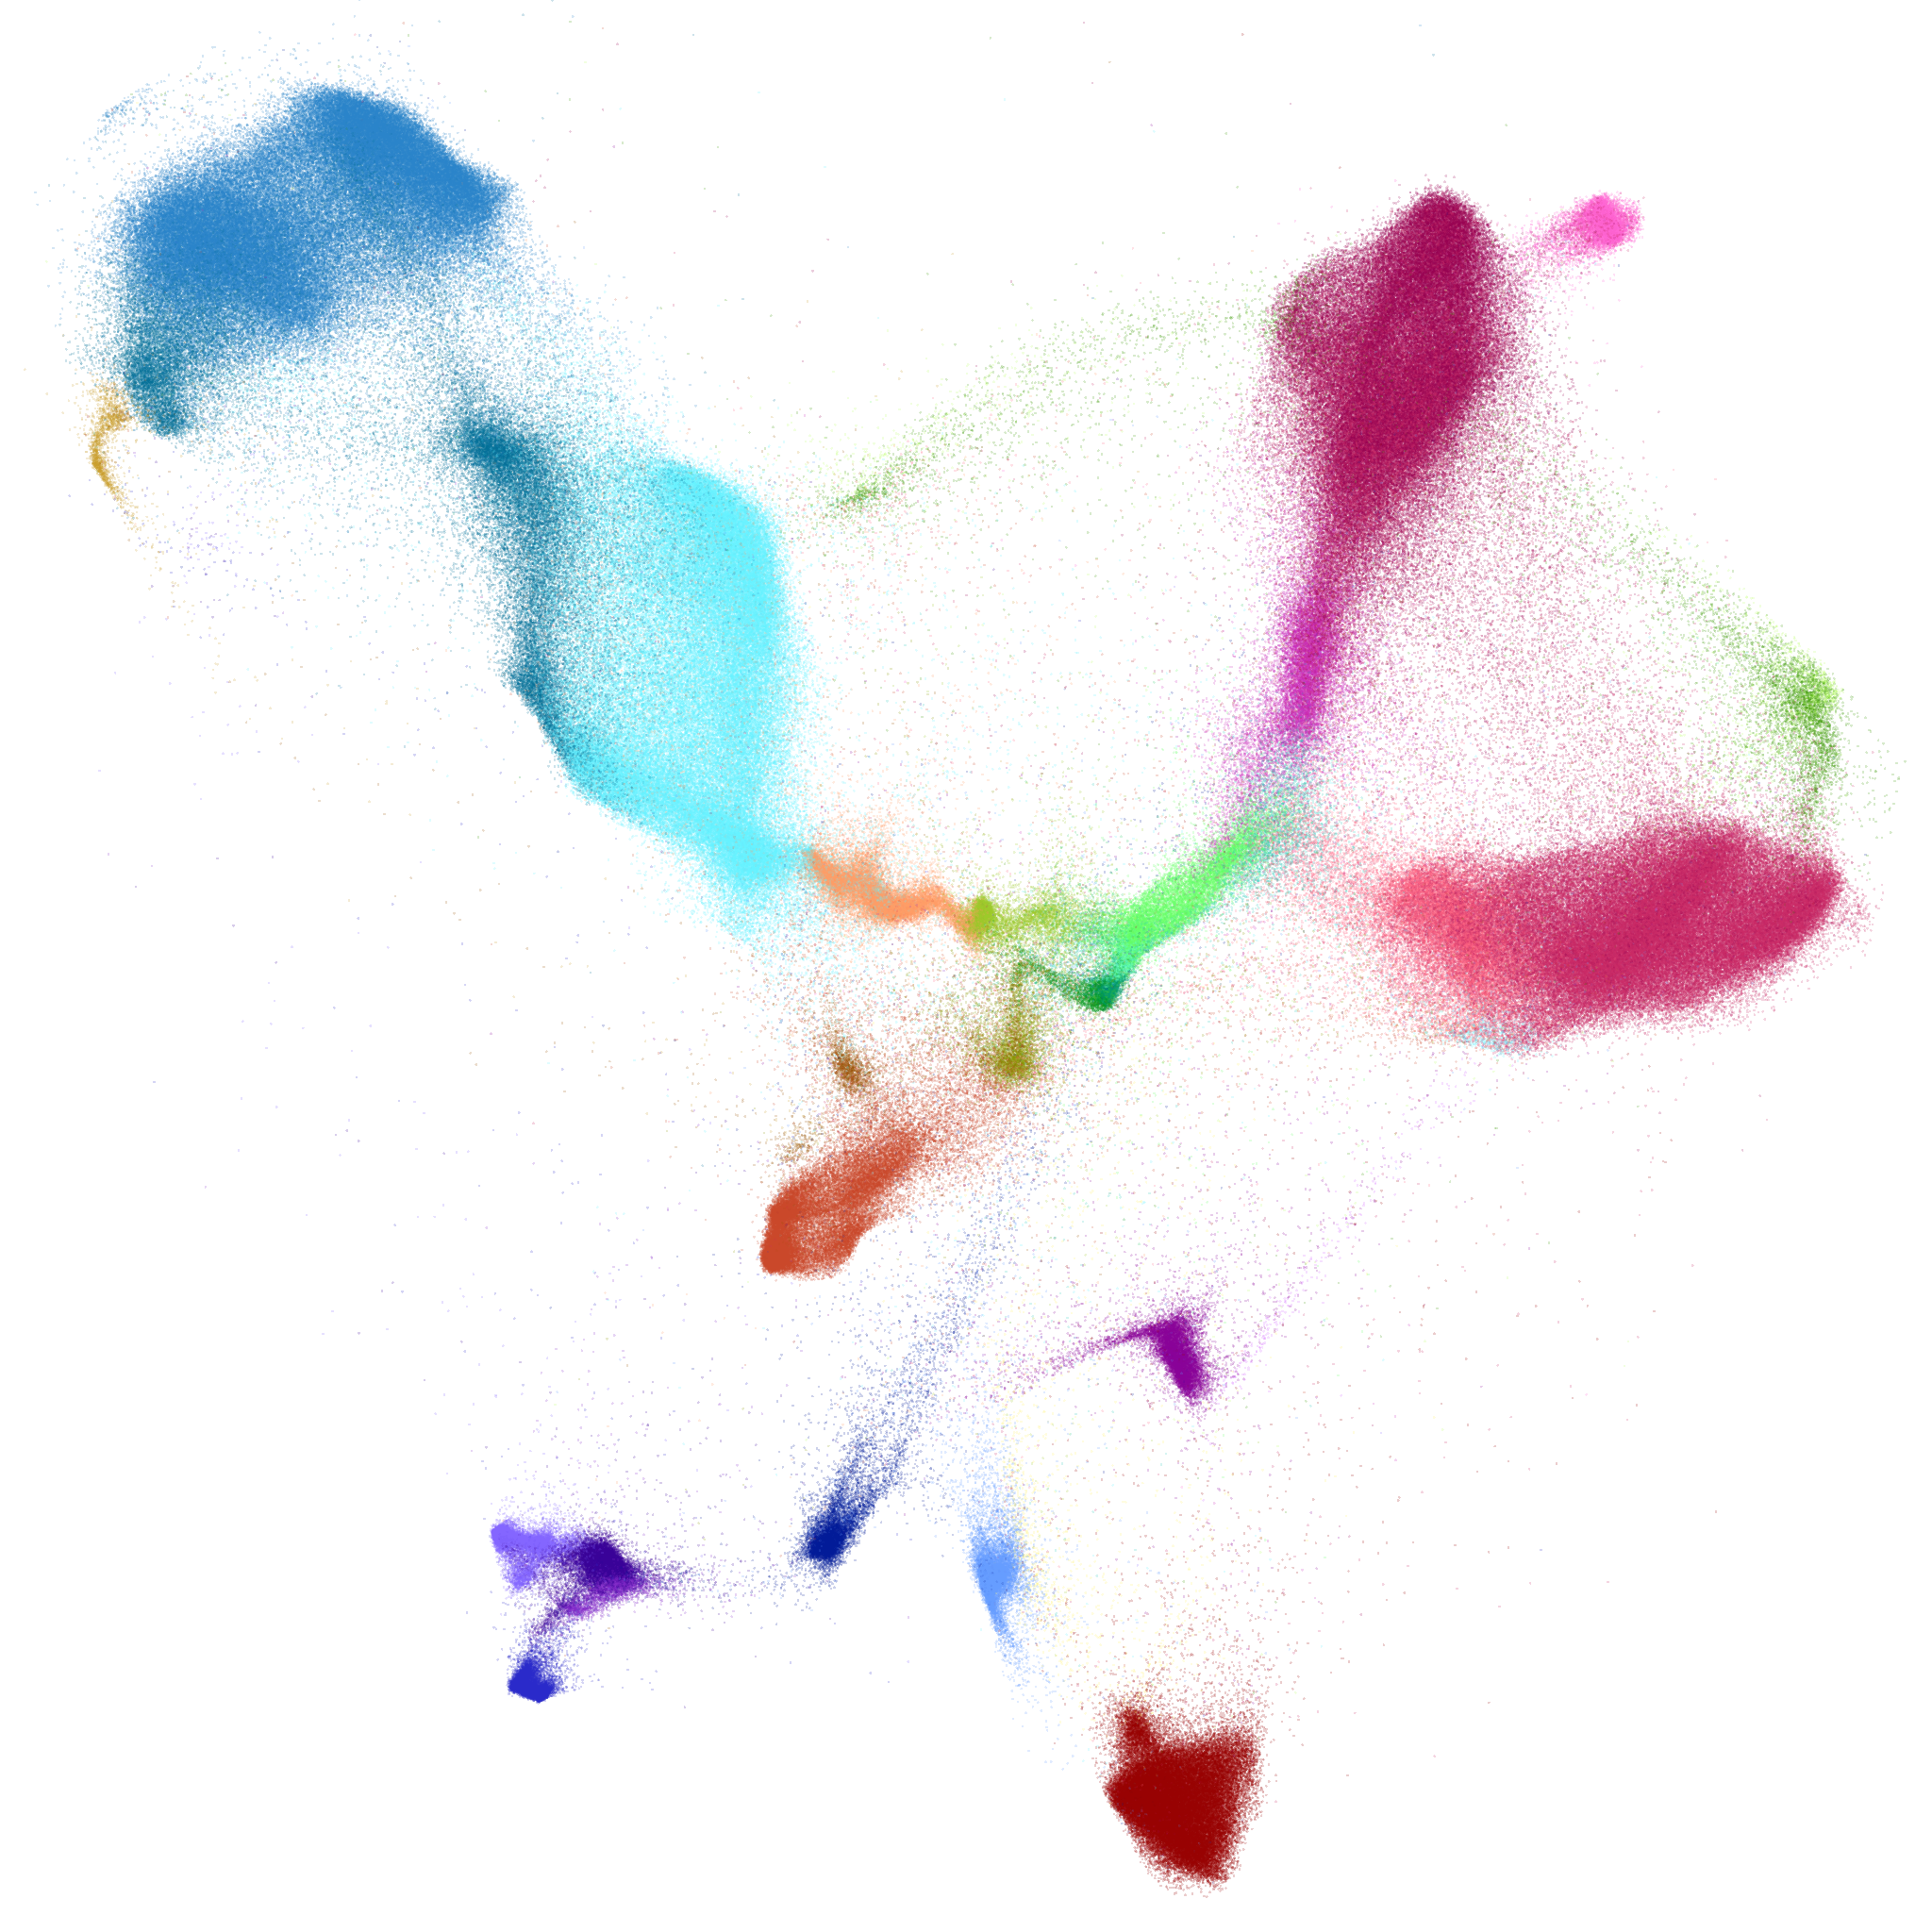
\includegraphics[width=\linewidth]{embedsom/pic/samusik-embedsom.png}};
% %\draw[help lines, xstep=0.1\linewidth, ystep=0.1\linewidth] (img.south west) grid (img.north east);
% \node[circle, draw] (A) at (0.5\linewidth,0.9\linewidth) {A};
% \node[circle, draw] (B) at (0.8\linewidth,0.2\linewidth) {B};
% \node[circle, draw] (C) at (0.2\linewidth,0.4\linewidth) {C};
% \node[circle, draw] (D) at (0.5\linewidth,0.266\linewidth) {D};
% \draw (A) to (0.45\linewidth,0.75\linewidth);
% \draw (A) to (0.9\linewidth,0.666\linewidth);
% \draw (B) to (0.55\linewidth,0.2\linewidth);
% \draw (B) to (0.65\linewidth,0.125\linewidth);
% \draw (B) to (0.55\linewidth,0.45\linewidth);
% \draw (C) to (0.5\linewidth,0.5\linewidth);
% \draw (C) to (0.275\linewidth,0.225\linewidth);
% \end{tikzpicture}}
% \caption{
% Example EmbedSOM projection of $841,644$ data points with $39$-dimensional single-cell measurements, representing the immune cell contents of bone marrow~\cite{samusik2016automated}. Colors were assigned manually to differentiate biologically relevant cell populations. Manual intervention in the unsupervised dimensionality reduction process would allow the user to fix several visualization deficiencies: overlapping pathways (labeled with~A), disconnected pathways (B), display of features in the small complex cell clusters (C), and the orientation and positioning of clusters that were chosen arbitrarily by the reduction process, not reflecting any biologically relevant features (D).
% }
% \label{fig:samusik}
% \end{figure}

% The development of non-linear dimensionality reduction algorithms in the last two decades has resolved many challenges. The new visualization-oriented methods, represented in the field mainly by t-SNE~\cite{maaten2008visualizing}, provided output that was sufficiently intuitive to understand, yet gave a satisfactory view of the highly complicated features that can not be observed by gating and projections. The tremendous success was quickly followed by new alternative algorithms that optimize different aspects of the process. UMAP~\cite{becht2019dimensionality} is currently a common choice for both visualization and a starting point of analysis, followed by PHATE~\cite{moon2019visualizing}, scvis\cite{ding2018interpretable}, TriMap\cite{amid2019trimap}, and others. For illustration, a typical example visualization is provided in~Figure~\ref{fig:samusik}, along with the description of common visualization problems.

% Following the plethora of newly introduced algorithms, a discussion unfolded to assess the optimality of the obtained visualization. Reviews have focused not only on reproducibility and robustness (i.e., susceptibility to significant changes in output caused by minor variations in data or different random seeds) but also on the representation of biologically valid features. Vast resources were invested into modifying the algorithms, especially t-SNE, to maximize various metrics, including convergence speed~\cite{belkina2019automated}, general performance~\cite{linderman2019fast}, robustness~\cite{polivcar2021embedding}, and the (very informally specified) quality of the display of local and global relations in data~\cite{kobak2019heavy,kobak2021initialization}. Some features required for high visualization quality are showcased in~Figure~\ref{fig:samusik}.

% User interaction possibilities in the dimensionality reduction process were therefore largely neglected, except for prohibitively small datasets where the use of force-based graph layouts and similar algorithms did not pose a throughput challenge. As one of few exceptions, van~Unen~et~al.~\cite{unen2017visual} and Chatzimparmpas~et~al.~\cite{chatzimparmpas2020t} achieved a methodological advance by extending the t-SNE algorithm, producing HSNE and t-viSNE respectively. HSNE organizes and visualizes a small data model dynamically using t-SNE, providing an intuitive way for the user to zoom into various compartments of the dataset, following a hierarchical structure of clusters. t-viSNE focuses on interactive use of t-SNE for exploration of complex dataset properties, but only of relatively small datasets.

% Compared to HSNE, our developments in BlosSOM provide two significant improvements: Full dataset may be rendered at all times (giving an unprecedented high-definition view of the features), which is enabled by a more efficient design of the base algorithm. Additionally, no hierarchical structure or no fixed layouting algorithm is imposed on the user, improving the display of structures that are hard to visualize or capture with hierarchical methods, such as the inter-cluster pathways.


% \subsection{GPU acceleration}

The essential component of our success is GPU acceleration of the projection computation which needs to be fast enough to re-calculate the embedding in real-time. 
In the following, we address the most relevant works that influenced or inspired our solution.

% One of the first GPU-accelerated dimensionality reduction methods was proposed in the work of Yeh et al.~\cite{yeh2010efficient} about twelve years ago. The first part uses $k$NN search with $k$-$d$-tree indexing structure. The GPU was used to compute Euclidean distances and to construct the tree using the radix sort algorithm. The projection itself used the Krylov subspace method for local linear embedding (LLE), which can be realized as a sparse matrix-vector multiplication so it was computed by cuBLAS. Despite the limited properties of the GPUs of the time, they were able to achieve $30$--$60\times$ speedup to the CPU implementation.

% A slightly different approach takes methods based on \emph{Principal Component Analysis} (PCA) algorithm. These methods are quite popular mainly since the principal components can be computed as eigenvectors of the data covariance matrix; thus, it can be implemented using linear algebra libraries. Martel et al.~\cite{martel2018implementation} proposed the implementation of PCA for CUDA and FPGAs. They have used the Jacobi method for the eigenvector decomposition, and the implementation heavily relied on Thrust and cuBLAS libraries. PCA is also used in more elaborate projection methods such as \emph{secant-based dimensionality reduction}~\cite{kvinge2018gpu}. The PCA is used to initialize a projection matrix, which is subsequently iteratively improved by a \emph{secant set} --- a set of normalized differences of all input point pairs. The projection matrix is multiplied with every secant to find a \emph{secant projection} with minimal $L_2$ norm. Although this method is theoretically intriguing, the GPU implementation is quite straightforward, using simple kernels and the cuSolver library.

Being one of the most profound visualization methods, \emph{t-SNE} was studied to explore the possibilities of having a fast GPU-enabled implementation. One of the initial implementations was t-SNE-CUDA library~\cite{chan2018t}. The most complicated step (computing the attractive forces of the N-body simulation) is handled as a multiplication of a sparse matrix and a vector by the CUSparse library. This work was slightly improved a year later \cite{chan2019gpu} when the authors replaced the CUSparse library with their implementation of multiplication, which takes advantage of atomic operations to perform the reduction in scalar sums.

% t-SNE can be improved by applying a hierarchical approach which can help both with the stability of the results and the computational demands of the algorithm. One of the first representatives that used a hierarchical approach and GPU acceleration was the Anchor-t-SNE (AtSNE) algorithm~\cite{fu2019atsne} which uses anchor points, selected representatives of the data which are projected first, and the remaining points are projected based on their proximity to the anchor points. A similar idea is used in the Barnes-Hut approximation of t-SNE\cite{van2014accelerating} which constructs a tree data structure that helps compute repulsive forces. This method was used in the work of Meyer et al.~\cite{meyer2020improving}, who implemented a warp-optimized CUDA version SWW-tSNE. Unlike the original t-SNE-CUDA, they have decided to use cuBLAS for the computation of attractive forces. The SWW-tSNE was later improved and accompanied with SWW-AtSNE~\cite{meyer2022global}, a warp-optimized version of anchor-based implementation of t-SNE~\cite{fu2019atsne}.

Perhaps the most popular contemporary method for data visualization is the \emph{Uniform Manifold Approximation and Projection} algorithm (UMAP), which often produces better results than t-SNE at the cost of higher computational demands. There are two GPU implementations worth mentioning which were both made part of RAPIDS cuML library~\cite{tegegne2021parallel, nolet2020bringing}. They both use a similar approach, implementing a kNN approximation based on gradient descent methods. The first implementation~\cite{tegegne2021parallel} relies more on existing solutions and libraries, and the second one~\cite{nolet2020bringing} is slightly more low-level as they implement the embedding using custom kernels.

Even though the presented methods (especially t-SNE) exceeded the speedup of two orders of magnitude, they are still quite far from real-time processing when the number of points reaches the order of millions. The proposed EmbedSOM projection is based on SOMs and linear projection based on $k$NN search~\cite{kratochvil2019generalized,kratochvil2020shinysom}, which is technically closest to the work of Yeh et al.~\cite{yeh2010efficient}. For the SOM part, we have adapted the state-of-the-art implementation of $k$-means algorithm~\cite{krulis2020detailed} since SOM shares many of its steps. The crucial part of the projection is the $k$NN search, which is also repeated in the aforementioned papers; however, we have found that the solution based on bitonic-sorting~\cite{krulivs2015optimizing} performs the best in our case.


\section{Conclusion}\label{sec:outro}

We have presented a GPU implementation for the semi-supervised dimensionality reduction algorithm EmbedSOM where we optimized independently two kernels: A general $k$NN search and a 2D projection which may be used independently. The $k$-NN was solved by adapted bitonic sorting, which eliminates thread divergence. The projection kernel was optimized to fetch and use data most efficiently by utilizing vector loads and data reuse on the register level. A thorough benchmarking indicates that both kernels achieved a significant speedup over the baseline GPU implementation.

The proposed implementation should enable subsequent research in interactive dimensionality reduction tools where the user changes SOM parameters or landmarks and the projections are re-computed and visualized in real-time. The results show that the optimized EmbedSOM version can project more than $1$ million individual data points each frame, while maintaining a frame rate above 30fps. 



% We have presented BlosSOM, a novel software for semi-supervised dimensionality reduction and visualization of large datasets.
% BlosSOM utilizes a GPU-accelerated implementation of the EmbedSOM algorithm as a highly efficient base for projecting the data to 2D, and improves its use with several supervision methods that allow the users to interactively and intuitively steer the process towards the desired solution with feedback.

% The GPU implementation in CUDA was thoroughly benchmarked and optimized.
% In BlosSOM, it is used to dynamically project the data points in an interactive visualization environment, where it re-projects and re-renders all data points every frame at high frame rate.
% On typical datasets, the optimized version is able to project more than 1 million of individual data points each frame, while maintaining a frame rate of 30fps or higher.

% We described and implemented several methods for user interaction with the landmark-based data model in EmbedSOM, based on self-organizing maps and graph embedding.
% The combination of the approaches in BlosSOM provided a solution to several challenges typically encountered with unsupervised dimensionality reduction.
% Finally, we demonstrated the use of BlosSOM on a biologically relevant use-case from single-cell cytometry, where it gives an effective way to produce desirable visualizations with variable level of details.

% We believe that the presented methodology will find use in explorative analysis of complex datasets, and provide a base for constructing intuitive, user-friendly annotation and dissection tools for single-cell cytometry data.

% \subsection{Data and software availability}\label{ssec:data}

% BlosSOM is available as free and open-source software from \texttt{https://github.com/\-molnsona/\-blossom}.
% Benchmark results are available from \texttt{https://github.com/\-asmelko/\-embed\-som-bench\-marks}.

% Datasets displayed in Sections \ref{sec:methods} and \ref{sec:results} are available from FlowRepository (\texttt{http://flow\-repository.org/\-id/FR-FCM-ZZPH}, file \texttt{Samusik\_all.fcs}) and from Smithsonian institute 3D digitization repository (\texttt{https://3d.si.edu/}, datasets `Mammuthus primigenius (Blumbach)' and `Tyrannosaurus rex', the 3D point coordinates were extracted manually from the vertex coordinates available in \texttt{.obj} files).


%%
%% The acknowledgments section is defined using the "acks" environment
%% (and NOT an unnumbered section). This ensures the proper
%% identification of the section in the article metadata, and the
%% consistent spelling of the heading.
% \begin{acks}
%   This paper was supported by Charles University institutional funding SVV 260698/2023.

% \end{acks}



\chapter*{Conclusion}
\addcontentsline{toc}{chapter}{Conclusion}


%%% Bibliography
%%% Bibliography (literature used as a source)
%%%
%%% We employ bibTeX to construct the bibliography. It processes
%%% citations in the text (e.g., the \cite{...} macro) and looks up
%%% relevant entries in the bibliography.bib file.
%%%
%%% The \bibliographystyle command selects, which style will be used
%%% for references from the text. The argument in curly brackets is
%%% the name of the corresponding style file (*.bst). Both styles
%%% mentioned in this template are included in LaTeX distributions.

\bibliographystyle{plainnat}    %% Author (year)
% \bibliographystyle{unsrt}     %% [number]

\renewcommand{\bibname}{Bibliography}

%%% Generate the bibliography. Beware that if you cited no works,
%%% the empty list will be omitted completely.

\bibliography{bibliography}

%%% If case you prefer to write the bibliography manually (without bibTeX),
%%% you can use the following. Please follow the ISO 690 standard and
%%% citation conventions of your field of research.

% \begin{thebibliography}{99}
%
% \bibitem{lamport94}
%   {\sc Lamport,} Leslie.
%   \emph{\LaTeX: A Document Preparation System}.
%   2nd edition.
%   Massachusetts: Addison Wesley, 1994.
%   ISBN 0-201-52983-1.
%
% \end{thebibliography}


%%% Figures used in the thesis (consider if this is needed)
\listoffigures

%%% Tables used in the thesis (consider if this is needed)
%%% In mathematical theses, it could be better to move the list of tables to the beginning of the thesis.
\listoftables

%%% Abbreviations used in the thesis, if any, including their explanation
%%% In mathematical theses, it could be better to move the list of abbreviations to the beginning of the thesis.
\chapwithtoc{List of Abbreviations}

%%% Doctoral theses must contain a list of author's publications
\chapwithtoc{List of publications}

%%% Attachments to the doctoral thesis, if any. Each attachment must be
%%% referred to at least once from the text of the thesis. Attachments
%%% are numbered.
%%%
%%% The printed version should preferably contain attachments, which can be
%%% read (additional tables and charts, supplementary text, examples of
%%% program output, etc.). The electronic version is more suited for attachments
%%% which will likely be used in an electronic form rather than read (program
%%% source code, data files, interactive charts, etc.). Electronic attachments
%%% should be uploaded to SIS and optionally also included in the thesis on a~CD/DVD.
%%% Allowed file formats are specified in provision of the rector no. 72/2017.
\appendix
\chapter{Attachments}

\section{First Attachment}

\openright
\end{document}
